% preamble for the RiTeh thesis template

\documentclass[botnum,a4paper,11,oneside,final]{tex_aux/rithesis}
%\usepackage[latin1]{inputenc}
%\usepackage[T1]{fontenc}
%\usepackage[english]{babel}
%%%%%%% adjustment for croatian
\usepackage[croatian]{babel}
\usepackage[cp1250]{inputenc}	% this ensures croatian special letters are correctly printed with Windows
%\usepackage[utf8]{inputenc}		% allegedly this will produc Croatian special letter correctly in Linux
%::::::::::::::::::::::::::::::::::::::::::::::::::::::::::::::::::::::::::::

\usepackage{enumitem}  % za reguliranje vertikalnoga razmaka izmedju stavki u listi
%\setlist{noitemsep} % or \setlist{nolistsep} to cancel all separations
\setlist[itemize]{itemsep=0pt, topsep=4pt, partopsep=0pt, parsep=1ex}
\setlist[enumerate]{itemsep=0pt, topsep=4pt, partopsep=0pt, parsep=1ex}
\setlist[description]{itemsep=0pt, topsep=4pt, partopsep=0pt, parsep=1ex}
%\setlist[enumerate,1]{leftmargin=1cm}
%\setlist[enumerate,2]{leftmargin=1.5cm}
%::::::::::::::::::::::::::::::::::::::::::::::::::::::::::::::::::::::::::::
%\usepackage{datetime}  % automatic months, years, days
%\newcommand{\MONTH}{%
%  \ifcase\the\month
%  \or sije�anj% 1
%  \or velja�a% 2
%  \or o�ujak% 3
%  \or travanj% 4
%  \or svibanj% 5
%  \or lipanj% 6
%  \or srpanj% 7
%  \or kolovoz% 8
%  \or rujan% 9
%  \or listopad% 10
%  \or studeni% 11
%  \or prosinac% 12
%  \fi}
%%::::::::::::::::::::::::::::::::::::::::::::::::::::::::::::::::::::::::::::
%\usepackage{setspace}
%\usepackage{lipsum,lineno}
\usepackage[pangram]{blindtext}
\usepackage{ragged2e}   % poravnavanje teksta
\usepackage{graphicx}	% this enables import of graphics
\usepackage[labelsep=space,format=hang]{caption}  % adjusts caption style
\usepackage{subfig}	% this enables use of subfigures
\usepackage{amsmath}
\usepackage{amssymb}
%\usepackage{fancyhdr}
\usepackage{amsfonts}
%\usepackage{amsthm}
%\usepackage{pdfsync}
% This package is used to tell TeXShop where things are in the PDF file.
% Command-click at any spot in the PDF and it will jump to the corresponding
% location in the source file.
\usepackage{epsfig}		% to use eps figures; maybe not necessary to use here with Mac
\usepackage{epstopdf}	% this automatically converts any eps-figure into a pdf-figure
\usepackage[section]{placeins} % da slika ne upada u sljedeci section

\hyphenation{sko-ko-vi-toj}

\DeclareGraphicsRule{.tif}{png}{.png}{`convert #1 `dirname #1`/`basename #1 .tif`.png}	% this converts any tif-figure into a png-figure (Mac directly supports pdf, jpg, png, and mps formats, but additionally can use tif and eps when they are automatically converted in png, and pdf, respectively, using the above two packages
\DeclareGraphicsExtensions{.pdf,.jpeg,.jpg,.png}  % ekstenzije koje ne treba pisati uz ime slike
\graphicspath{{slike/}}   % mjesto gdje su smjestene slike

%\usepackage{makeidx}	% this enables creation of index
%\usepackage{showidx}
%\makeindex			% this makes index automatically, based on author's entries

%\usepackage{eufrak}
%\usepackage[mathcal]{euscript}
\usepackage{psfrag}
%\usepackage{url} 
\usepackage{hyperref}
\hypersetup{
breaklinks,
colorlinks=true,
linkcolor=black,
citecolor=black,
filecolor=black,
urlcolor=black
}

\setcounter{topnumber}{1} \setcounter{bottomnumber}{1}

\newcommand{\navod}[1]{``#1''}

\usepackage{glossaries}
\setacronymstyle{short-long}
\makeglossaries

%Custom dodano
\usepackage{spverbatim}
\usepackage{indentfirst}
\usepackage{listings,xcolor}
\usepackage{inconsolata}
\usepackage{amsmath}
\usepackage[noend]{algpseudocode}

\usepackage[chapter]{algorithm}
\floatname{algorithm}{Pseudokod}

\usepackage[labelfont=it,textfont=it]{caption}
\renewcommand{\lstlistingname}{Kod}
\renewcommand{\lstlistlistingname}{Popis isje�aka koda}
\renewcommand{\listalgorithmname}{Popis pseudokodova}

\usepackage{float}
\usepackage{pdfpages}

\lstdefinestyle{myC++}{
    language        = C++,
    basicstyle      = \fontsize{9}{11}\ttfamily,
    %keywordstyle    = \color{dkblue},
    %morekeywords	= {function,return,public,class,protected,interface,as,new},
    %stringstyle     = \color{red},
    %identifierstyle = \color{dkgreen},
    %commentstyle    = \color{gray},
    captionpos 	    = b,
    % emph            = [1]{__construct},
    %emphstyle       = [1]\color{dkgreen},
    numbers=left, 
    xleftmargin=2.5em,
    numberstyle=\small, 
    %numbersep=8pt, 
    frame = single,
    framexleftmargin=2.5em,
    breaklines=true
}

\colorlet{punct}{red!60!black}
\definecolor{background}{HTML}{EEEEEE}
\definecolor{delim}{RGB}{20,105,176}
\colorlet{numb}{magenta!60!black}

\lstdefinelanguage{json}{
	basicstyle=\normalfont\ttfamily,
	numbers=left,
	numberstyle=\scriptsize,
	stepnumber=1,
	numbersep=8pt,
	showstringspaces=false,
	breaklines=true,
	frame=lines,
	literate=
	*{0}{{{\color{numb}0}}}{1}
	{1}{{{\color{numb}1}}}{1}
	{2}{{{\color{numb}2}}}{1}
	{3}{{{\color{numb}3}}}{1}
	{4}{{{\color{numb}4}}}{1}
	{5}{{{\color{numb}5}}}{1}
	{6}{{{\color{numb}6}}}{1}
	{7}{{{\color{numb}7}}}{1}
	{8}{{{\color{numb}8}}}{1}
	{9}{{{\color{numb}9}}}{1}
	{:}{{{\color{punct}{:}}}}{1}
	{,}{{{\color{punct}{,}}}}{1}
	{\{}{{{\color{delim}{\{}}}}{1}
	{\}}{{{\color{delim}{\}}}}}{1}
	{[}{{{\color{delim}{[}}}}{1}
	{]}{{{\color{delim}{]}}}}{1},
}




% pomocu \includeonly moze se kompajlirati samo odredjeno poglavlje, da se skrati vrijeme kompajliranja, dok se ne isprave pogreske u tom poglavlju npr.:
%\includeonly{Poglavlje_1}

\begin{document}

\frontmatter   % - ne dirati

% upisati naziv studija
\degreesubject{Diplomski sveu�ili�ni studij ra�unarstva} % upisati odgovarajuci naziv studija

% upisati vrstu rada
\documenttype{Diplomski rad}  % Zavrsni rad ili Diplomski rad

\title{Pro�iriva univerzalna paleta aplikacijskih komandi za interakciju zasnovanu na tipkovni�kim pre�acima}   % upisati specificni naslov rada

\date{\MONTH~\the\year.}   % ne dirati - mjesec i godina ?e se upisati sami

\author{Tomislav Milanovi�}  % upisati svoje ime i prezime
\jmbag{0069069002}  % upisati vlastiti JMBAG
\maketitle		% ne dirati //komentirati ako se ?eli da bude samo jedna stranica

%\makecopyright

% Okruzenje za pisanje posvete. Maknuti komentare ukoliko se ?eli napisati posvetu.
%\begin{dedication}
%	Ovo je posveta nekome
%\end{dedication}

\mentor{doc. dr. sc.~Sandi Ljubi�}   % zamijeniti podacima o svojem mentoru
\maketitleabstract

% kreira mjesto za umetnuti stranicu s opisom zadatka - ne dirati
\addtolength{\topmargin}{-1.0cm}
\begin{figure}
    \begin{center}
    
\includegraphics[width=1.0\textwidth,height=1.0\textheight,keepaspectratio]{diplomski}    
    \end{center}
\end{figure}




%\begin{assignmentpage}
    %\addtolength{\topmargin}{-1.0cm}
\begin{figure}
    \begin{center}
    
\includegraphics[width=1.0\textwidth,height=1.0\textheight,keepaspectratio]{diplomski}    
    \end{center}
\end{figure}




%\end{assignmentpage}

% kreira mjesto za umetnuti stranicu s izjavom o samostalnoj izradbi zadatka - ne dirati
\begin{honestystatementpage}
	

{ \large 
\vspace{15pt}
% prilagodite ovu izjavu s obzirom na potrebni rod imenice (izradio ili izradila)
%::::::::::::::::::::::::::::::::::::::::::::::::::::::::::::::::::::::::::::::::
Sukladno �lanku 9. Pravilnika o zavr�nom radu i zavr�nom ispitu na preddiplomskim sveu�ili�nim studijima i stru�nim studijima Tehni�kog fakulteta Sveu�ili�ta u Rijeci, izjavljujem da sam samostalno izradio zavr�ni rad na temu: Implementacija algoritma za pra�enje zrake svjetlosti prema zadatku: Klasa: 602-04/17-04/18, Ur.br.: 2170-15-11-17-2, zadanom u Rijeci, 23.3.2017.\vspace{7cm} \\ 

%::::::::::::::::::::::::::::::::::::::::::::::::::::::::::::::::::::::::::::::::
% ovo ispod nema potrebe dirati!
%:::::::::::::::::::::::::::::::::::::::::::::::::::::::::::::::::::::::::::::::::::
\noindent Rijeka, \MONTH~\thisyear.   
\hspace{5.5cm}
	\verb|__________________|  % pomo�u duzine ove crte regulirati potrebnu sirinu crte za potpis

\begin{flushright}
	\vspace{-15pt}
	Tomislav Milanovi� 
	\verb|   |   % pomocu praznih mjesta unutar | | crta, regulirati poravnjanje duzine imena i prezimena s gornjom crtom za potpis
\end{flushright}
%:::::::::::::::::::::::::::::::::::::::::::::::::::::::::::::::::::::::::::::::::::

} % \large
\end{honestystatementpage}

% Okruzenje za pisanje zahvale
\begin{acknowledgments} % staviti znak komentara ukoliko se ne stavlja tekst zahvale
	\vspace{5pt}

%\begin{flushleft}
\noindent Zahvaljujem se mentoru doc. dr. sc. Sandiju Ljubi�u na pru�enim konzultacijama za ovaj rad te na pomo�i pri tra�enju zainteresiranih sudionika istra�ivanja. Zahvaljujem se svim sudionicima koji su se odazvali. Bez vas ovaj rad ne bi bilo mogu�e realizirati. Puno hvala kolegi Dinu Ili�u na korisnim savjetima. Tako�er, zahvaljujem se obitelji na podr�ci tijekom cjelokupnog studiranja.
%\end{flushleft}  
\end{acknowledgments}

% kreiranje popisa sadrzaja, slika i tabela - ni?ta ne dirati
\tableofcontents
%\listoffigures
%\listoftables

\mainmatter		% ne dirati

% Ovdje pomo?u include funkcije ucitavati kreirana poglavlja. Poglavljima dajte logicna imena s obzirom na sadrzaj prikazan u njima (bez razmaka u imenu).
%\chapter{Kako koristiti paket za pisanje zavr�noga rada u \LaTeX-u}
Ovo su uvodne napomene za kori�tenje predlo�ka za pisanje zavr�noga ili diplomskoga rada studenata Tehni�koga fakulteta u Rijeci. Prije kori�tenja paketa, pro�itajte ovaj tekst jer �e vam dati nu�ne uvodne informacije, znatno vam olak�ati i ubrzati ure�ivanje teksta nakon toga, pri �emu �e vas i voditi kroz uporabu ovoga paketa na prakti�an na�in.

Paket je pripremljen tako da student �to prije mo�e pisati vlastiti tekst u ve� pripremljenom predlo�ku koji �e, uz minimalno u�enje sintakse \LaTeX-a, studentu olak�ati urediti svoj rad. U paketu su uklju�ene potrebne upute i sintakti�ke strukture koje bi trebale udovoljiti potrebama ve�ine studenta, a dodatne informacije postoje u dvama priru�nicima koji su uklju�eni u ovom paketu te, naravno, na raznim web stranicama na internetu koje su posve�ene \LaTeX-u (vidi u nastavku).

{\color{red} POZOR: paket treba biti prekopiran negdje na disk ne mijenjaju�i originalnu strukturu mapa (foldera) i ne mijenjaju�i nazive datoteka koje su u mapi \emph{tex\_aux}!}


\section{Opis sadr�aja paketa}
\vspace{-2ex}
Paket se sastoji od:
\begin{itemize}
 \item datoteke \href{run:UPUTE.pdf}{{\color{blue} UPUTE.pdf}} koja sadr�i postupak instalacije potrebnih alata na ra�unalo te kori�tenja paketa. \emph{UPUTE} su bazirane na Windows OS, a korisnici drugih OS-ova si na nazna�enim web lokacijama samo trebaju na�i instalacije za njihov OS.
 %
 \item datoteke \verb|JMBAG_Ime_Prezime.tex| koja je sredi�nja datoteka koja povezuje sve cjeline i kompajliranjem koje se dobije izlazni \verb|JMBAG_Ime_Prezime.pdf| dokument (naravno, tijekom rada, upisat �ete svoj specifi�ni JMBAG i ime i prezime).\\ U ovoj se datoteci inicijalno nalaze i upute za kori�tenje paketa kao i primjeri osnovne uporabe naj�e��ih sintakti�kih struktura u \LaTeX-u koje bi trebale biti dovoljne ve�ini studenata za pisanje rada.
 %
 \item mape \verb|tex_aux| u kojoj su \emph{interne datoteke} koje definiraju stilove, formate i sl.\ koji slu�e u slaganju izlaznoga formata. \textbf{Student/ica s njima ne treba \emph{ni�ta} raditi}, ali one trebaju biti u \verb|tex_aux| mapi pod glavnom mapom zavr�noga rada, kao �to je postavljeno u ovom paketu.
 %
 \item mape \emph{slike} u koju student treba pohraniti sve slike koje �e koristiti u radu. Ime mape se ne smije preimenovati bez boljega poznavanja sintakse \LaTeX-a jer ovaj paket da bi ispravno radio o�ekuje ba� takvo ime mape!
 %
 \item datoteke \verb|sintaksa_cestih_struktura.tex| koja ne sudjeluje izravno u kompajliranju pdf dokumenta, nego slu�i kao repozitorij u kojemu su sadr�ane naj�e��e potrebne sintakti�ke strukture koje su spremne za kopiranje u va� tekst uz minimalnu prilagodbu parametara (npr.\ opis slike, ime datoteke specifi�ne slike koju se ubacuje i proizvoljni ID te slike za kasnije referenciranje).
 %
 \item mape \href{run:prirucnici}{{\color{blue}prirucnici}} u kojoj se nalazi nekoliko najpopularnijih priru�nika za uporabu \LaTeX-a. 
\end{itemize}
%%%%%%%%%%%%%%%%%%%%%%%%%%%%%%%%%%%%%%%%%%%%%%%%%%%%%%%%%%%%%%%

\section{�ime se opremiti za pisanje rada}
Da bi se rad napisao pomo�u \LaTeX-a (a to vrijedi svake lipe!), najprije je na ra�unalo potrebno instalirati:
\begin{enumerate}
	\item obavezno: \LaTeX{} software 
	\item obavezno: editor za ure�ivanje teksta 
	\item neobavezno, ali korisno: softver za opis literature. (Premda dodatni softver nije nu�an jer se popis literature mo�e obraditi i ru�no (no to je manje sofisticirano kod uvr�tavanja referenca), sugeriram instalaciju softvera koji pomo�u intuitivnih su�elja korisniku omogu�ava opis pojedine kori�tene literature (kao mala baza podataka), a potom se pojedina jedinica literature jednostavno ubacuje u tekst, a popis literature se na kraju automatski formira (vi�e o tome pro�itajte u nastavku).
\end{enumerate}

\subsection{Instalacija \LaTeX-a}
\begin{enumerate}
	\item odite na sredi�nji \LaTeX{} portal \cite{latex_project}: \url{http://www.latex-project.org/}
	\item kliknite na poveznicu \href{http://www.latex-project.org/ftp.html}{Getting LaTeX} i potom uo�ite i povucite instalaciju koja odgovara va�em OS-u (npr.\ proTeXt za Windows, MacTeX za Mac, TeX Live za Linux). Pozor: instalacijski paket je velik i mo�e du�e potrajati �ak i na brzoj vezi---dajte si dovoljno vremena za obaviti download.
	\item Instalirajte \LaTeX{} slijede�i upute koje su prilo�ene za odabranu instalaciju (npr.\ proTeXt za Windowse daje kratki pdf s uputama koje vas vode kroz instalaciju korak po korak).
\end{enumerate}

\subsection{Instalacija editora teksta}
Instalirajte editor koji je pogodan za pisanje \LaTeX{} koda. \textbf{Za Windows OS, toplo preporu�am}  \href{http://www.texstudio.org}{{\color{blue} TeXstudio}} \cite{texstudio} jer je bogat opcijama, ugodan za rad i stabilan, a instalacije postoje i za Linux i Mac OS. TeXstudio se zasebno povu�e i instalira na ra�unalo, a neke editore teksta koji ve� do�u u paketu za instalaciju LaTeXa mo�ete ignorirati (npr.\ za Windows je do nedavno bio popularan \emph{TeXnicCenter} i dolazi ve� upakiran u proTeXt-u (a mo�da �ete na�i i \emph{TeXworks}), za Mac je kvalitetan \emph{TeXShop} koji sada tako�er dolazi u paketu s MacTeX-om). 

\label{encoding1} {\color{red} POZOR: Premda �e ovo biti jo� napomenuto na stranici~\pageref{encoding2}, prije samoga po�etka pisanja va�ega rada, �to prije �elim napomenuti sljede�i va�ni detalj: za svaki va� tekst koji pi�ete u editoru teksta, uvjerite se da je kodna stranica postavljena na \navod{windows-1250}, �to je klju�no da bi se u izlaznom pdf-u ispravno ispisivali hrvatski dijakriti�ki znakovi! U TeXstudiu, aktualnu kodnu stranicu se mo�e vidjeti i promijeniti preko maloga izbornika u doljnjem desnom kutu glavnoga prozora, gdje se nalazi opcija ``Encoding''. Ukoliko tu ne pi�e ``windows-1250'', kliknite na izbornik, odaberite opciju ``More Encodings'' pa u potom otvorenom su�elju odaberite kodnu stranicu ``windows-1250 / CP 1250'' i potvrdu sa ``Change To''.}

\subsection{Instalacija programa za opis kori�tene literature}
\emph{Ponavljamo: Kori�tenje BiBTeX programa za opis literature \textbf{nije} neophodno, ali jest korisno. U datoteci po imenu \href{run:Literatura.tex}{{\color{blue}Literatura.tex}}, koja je uklju�ena u ovaj paket, ve� su namje�tene postavke kao da �e se literatura opisati pomo�u BiBTeX programa (npr.\ JabRef-a) i ne treba ni�ta mijenjati, ali ispod toga se mo�e prona�i i upute i za drugi--ru�ni-- na�in (p)opisivanja literature.}

Kao bibtex program za opis literature, preporu�am \href{http://www.jabref.org}{{\color{blue} JabRef}} program \cite{jabref}. To je legalno besplatno dostupni program za Windows OS (ali postoji i za Mac, a i platformski neovisna instalacija) koji nam omogu�ava opisivanje literature na lak na�in pomo�u intuitivnih su�elja, a kao rezultat kreira \emph{BibTeX} datoteku \emph{Literatura.bib} (gdje je (\emph{Literatura} naziv koji korisnik treba dodijeliti pri pohrani JabRef datoteke na disk u slu�aju ovoga predlo�ka, da bi paket funkcionirao) u kojoj je literatura opisana na na�in koji \LaTeX{} razumije. 

Uo�ite da ako ne koristite JabRef, ve� se odlu�ite za ru�ni unos literature, �to se isprva doima jednostavnijim, tada �e vam redoslijed referenca u popisu literature odgovarati to�no redoslijedu koji ste naveli u tom popisu --- dakle morate paziti da redoslijed formirate onim redom kojim pozivate reference u va�em tekstu (�to kod nekog kasnije ubacivanja dodatne reference unutar ve� postoje�ega redoslijeda tra�i brigu da ju se ubaci na odgovaraju�e mjesto u popisu literature), a tako�er trebate paziti i na formatiranje teksta svake reference! 

Za razliku od toga, kori�tenjem JabRef-a, izbjegavate ru�no formiranje popisa literature i ne trebate brinuti o redoslijedu referenca, ve� samo pomo�u JabRefa trebate unijeti sve jedinice literature koju �ete navesti, a \LaTeX{} �e vam automatski formirati listu referenca onim redoslijedom kojim reference bude pozivali u tekstu!

Nakon �to kompajlirate projekt, stvorit �e vam se pomo�na datoteka imena \href{run:JMBAG_Ime_Prezime.bbl}{{\color{blue}JMBAG\_Ime\_Prezime.bbl}} u kojoj �e jedinice literature tijekom kompilacije biti formatirane i odatle se ubacuju u kona�nu verziju teksta. Stoga, \textbf{ukoliko ima ikakvih detalja koje u opisu literature treba prilagoditi, a ne mo�ete automatskim putem}, uvijek vam kao ``zadnja crta obrane'' ostaje otvoriti \verb|bbl| datoteku i tamo ru�no napraviti izmjene. Potom ponovo kompajlirajte projekt i te �e se promjene vidjeti u pdf-u tj.\ ru�no unijete promjene ne�e biti poni�tene sve dok ne obri�ete cijelu datoteku.

Umjesto da rukom pi�ete cijelu bibliografiju, vremenski vam je vjerojatno u�inko\-vitije popis literature generirate uporabom JabRef-a, a potom ako i�ta jo� treba prilagoditi, onda samo to napraviti ru�no u \verb|bbl| datoteci.


\subsubsection{Osnovna uporaba JabRef programa}
Upoznajte se s najva�nijim opcijama u \emph{JabRef}-u:
\begin{itemize}
	\item uo�ite ikonu (pod znakom ``+'' i tekstom \emph{New BibTeX Entry}) za unos nove jedinice literature (npr. knjige, �lanka, web portala i sl.)
	%
	\item kada kliknete za unos nove stavke literature, uo�ite kakvi se sve tipovi literature nude za odabir. Odabirom opcije koja odgovara naslovu koji �elite unijeti, otvorit �e vam se novi prozor s poljima u koja se mo�e unijeti informacije o literaturi. Za odabrani tip literature samo su neka polja obavezna (nalaze se pod karticom (eng.\ \emph{tabom}) \emph{Required fields}), dok se pod drugim karticama mo�e i ne mora unijeti dodatne informacije. U slu�aju na�ih zavr�nih/diplomskih radova, bit �e znatan udjeli literature koja je na internetu pa za formatiranje iste, pro�itajte upute i napomene u nastavku ove sekcije.
	%
	\item kada je vi�e autora, njihova imena se u JabRefu polju za unos autora razdvajaju pisanjem klju�ne rije�i \verb|and| (a ne razmakom, zarezom ili to�ka-zarezom!)
	%
	\item U popisu literature se ne�e uvijek pojam prepisati onako kako ste ga vi zapisali u JabRefu! To je posljedica stilova koji su definirani u \verb|bst| datoteci (ne zamarajte se time sada jer je za naprednu razinu \LaTeX-a). No, ako neki pojam ba� ne ispadne suvislo napisan u popisu literature ili ba� �elite forsirati odre�eni na�in zapisa (�esto slu�aj kada se rije� s velikim slovima ne interpretira onako kako �elite), tada to�no odre�eni zapis mo�ete forsirati na na�in da \verb|{tu rije� ili frazu stavite unutar viti�astih zagrada}|
	%
	\item prije nego pohranite pojedinu stavku pomo�u \emph{Ctrl+S}, \textbf{morate svakoj jedinici literature dodijeliti jedinstveni identifikator}, tzv.\ \emph{Bibtexkey}, �to je jedno od polja koja su obavezna za unos. Mo�ete ru�no upisati neki proizvoljni string, ali pogodnije je generirati ga automatski.\\ Za to u�initi me�u ikonama na vrhu imate ikonu koja izgleda kao (�arobni) �tapi� sa zvjezdicama oko njega, klikom na kojega \emph{JabRef} automatski dodijeli jedinstveni BibTeX \emph{klju�} za tu bibliografsku jedinicu. Pomo�u toga klju�a se poslije bilo kada i bilo gdje u pisanju va�ega rada mo�ete pozvati na tu referencu, a \LaTeX{} �e sve ostalo obaviti za vas tj.\ dodijeliti joj odgovaraju�i broj u tekstu i s tim brojem uvrstiti u popis literature.
	%
	\item korisnik ima mogu�nost i promijeniti uzorak po kojem se kreira struktura automatski generiranoga jedinstvenoga BibTeX klju�a tako da se otvori opcija izbornika \emph{Options $>>$ Preferences $>>$ BibTeX key generator}, gdje je na vrhu prozora prikazan \emph{default} uzorak, npr. \verb|[auth]:[year]| �to zna�i da se klju� kreira na bazi \verb|prezime(autora):godina(rada)|. To se sada mo�e urediti po nekom novom uzorku, no ovako definirani uzorak u biti zadovoljava, a ako igdje ima potrebe za dodatnim razlikovanjem, mo�e se na automatski generiranom klju�u jo� ru�no napraviti korekcija dodavanjem nekog znaka na kraju, kao npr.\ dodavanjem \verb|_a| i sl. (Klikom na karticu \emph{BibTeX source} mo�ete vidjeti kako �e unos va�ih podataka zapravo biti zapisan u va�oj \emph{Literatura.bib} datoteci koja �e se formirati od svih bibliografskih jedinica koje unesete.)
	%
	%
	\item Za \emph{ime} va�e bibliografske datoteke kod pohrane na disk obavezno upi�ite  \emph{Literatura} jer to ime o�ekuje ovaj paket. Pozor: Datoteka \emph{Literatura.bib}, koju ste tako kreirali, mora se nalaziti unutar mape ovoga paketa da bi sve ispravno radilo! U paketu je za primjer ve� kreirana jedna datoteka istoga imena koju za vje�bu student mo�e i otvoriti u \emph{JabRef}-u, ali to su samo pokazne bibliografske jedinice unesene kao primjer, koje student treba u kona�nici zamijeniti svojim bibliografskim jedinicama.
	%
	\item Za ``elektroni�ke'' izvore literature (tj.\ sve �to ste kao informaciju na�li na webu), JabRef nudi tip literature pod nazivom ``Electronic'' (vidi Sl.~\ref{fig:jabref}). U njemu pod karticom (eng.\ tabom) \emph{Optional fields} pod poljem \verb|Title| mo�ete upisati ime web stranice (autor, tvrtka i sl.), pod poljem \verb|url| mo�ete upisati URL adresu te web stranice, a pod poljem \verb|Note| upisati datum kada ste posjetili tu web stranicu (npr.\ \emph{srpanj 2016.} ili \emph{3.~rujna~2016.}). Rezultat toga �e u pdf-u biti da je sve napisano redoslijedom koji je predvi�en u Uputama RiTeha za pisanje diplomskog rada \cite{riteh_upute}, \emph{osim �to u ovom Predlo�ku do sada nisam uspio rije�iti ubacivanje zareza izme�u URL adrese i datuma posjeta toj URL adresi}, koji bi ta dva podatka odvojio, pa je tu potrebna mala ru�na \emph{prilagodba na jedan od ovih dvaju na�ina}:
	\begin{enumerate}[label=\textbf{\roman*)}]
		\item kod unosa datuma u polje \verb|Note| (u su�elju JabRef-a), upi�ite datum na sljede�i na�in: \verb|{, <datum>}|, gdje je \verb|<datum>| va� specifi�ni datum, dok �e \emph{zarez} iza prve zagrade izvr�iti razdvajanje URL adrese i datuma, a \textbf{viti�aste zagrade} osigurati da se to ba� tako to�no prenese u pdf-dokument (uklju�uju�i i da se mjesec napi�e malim po�etnim slovom, �to ina�e ne bi bio slu�aj). (Za neke druge tipove referenca kao npr.\ tip \emph{manual}, zarez vam prije datuma ne�e trebati jer �e naziv literature zavr�iti zarezom.) U Jabrefu vam i ina�e vrijedi da kada �elite forsirati da se pojam ba� to�no u popisu literature zapi�e onako kao ste htjeli, onda se pojam stavi unutar viti�astih zagrada \verb|{kao u ovom primjeru}|.
		\item ako u polju \verb|Note| ne upi�ete datum na prethodno opisani na�in, onda vam u pdf dokumentu ne�e biti upisan zarez izme�u URL adrese i datuma koji ste unijeli, a tako�er �e i mjesec biti napisan velikim po�etnim slovom (�to nije stra�no, ali je manje po�eljno). To mo�ete \emph{ru�no} prilagoditi tako da otvorite \verb|.bbl| datoteku i pomo�u \emph{Find/Replace} operacije sve nazive mjeseca zamijenite na na�in da po�inju malim po�etnim slovom (�to nije te�ko kada vam je ve�ina datuma u popisu literature navedena u istom mjesecu), ali zareze �ete svakako morati ubacivati ru�no u svaku pojedinu stavku literature jer ne�e biti nekog predlo�ka kojim biste to rije�ili automatski pomo�u \emph{Find/Replace} operacije. Na kraju opet kompajlirajte projekt. S obzirom na navedeno, prvi na�in je vremenski �tedljiviji!
	\end{enumerate}
\end{itemize}

%%%%%%%%%%%%%%%%%%%%%%%%%%%%%%%%%%%%%%%%%%%%%%%%%%%


\chapter{Primjeri naj�e��ih sintakti�kih struktura}
Prije stvarnoga po�etka pisanja svoga rada, upoznajte se s osnovnim sintakti�kim strukturama koje �e vam trebati tijekom pisanja rada.

U nastavku su opisane naj�e��e sintakti�ke strukture (dio njih mo�ete na�i i u datoteci \emph{Intro.tex}), a dodatne slo�enije strukture su pohranjene u datoteci \href{run:sintaksa_cestih_struktura.tex}{{\color{blue}sintaksa\_cestih\_struktura.tex}} koja je sastavni dio glave mape ovoga paketa. 

\section{Postavljanje naslova poglavlja i sekcija}
\begin{itemize}
	\item \verb|\chapter{Naslov poglavlja}|: za definiranje naslova poglavlja
	\item \verb|\section{Naslov sekcije}|: za definiranje naslova sekcije unutar poglavlja
	\item \verb|\subsection{Naslov podsekcije}|: za definiranje naslova podsekcije
\end{itemize}


\section{Reference na literaturu} \label{sec:RefLit}
Za referencu na pojedini kori�teni izvor informacije (tj.\ jedinicu literature), koristimo naredbu \\
\verb|\cite{bibtexkey}|, gdje je \emph{bibtexkey} jedinstveni klju� kojim prethodno ozna�imo tu jedinicu literature. \verb|Bibtexkey| mo�emo definirati na jedan od sljede�ih na�ina:
\begin{description}
	\item[I)] ako popis literature definiramo izravno u datoteci \href{run:Literatura.tex}{{\color{blue}Literatura.tex}} (opcija (I) u datoteci), onda ispred svake stavke literature treba definirati i jedinstveni \verb|bibtexkey| pomo�u naredbe \verb|\bibitem{bibtexkey}| (vidi predlo�ak u datoteci)
	\item[II)] ako literaturu opisujemo pomo�u JabRef datoteke \emph{Literatura.bib} (opcija (II) u datoteci), onda se tamo uz svaku stavku definira \verb|bibtexkey| (bude na dnu JabRef obrasca za upis pojedine jedinice literature)
\end{description}
%
Npr.\ ako negdje u tekstu napi�emo \verb|\cite{latex_wiki}|, gdje je \verb|latex_wiki| prethodno definirani \emph{bibtexkey}, tada �e se u tekstu u uglatoj zagradi pokazati broj  te bibliografske jedinice pod kojim se nalazi u popisu literature (Bibliografiji) na kraju rada (u ovom primjeru, to je broj \cite{latex_wiki}).


\section{Referenca na sekciju, sliku, tabelu ili stranicu} \label{sec:RefText}

Za referenciranje na pojedine dijelove teksta unutar rada, koristimo
{\color{red} \verb|\label{ID}|} i {\color{red} \verb|\ref{ID}|} na na�in da se \verb|\label{ID}| postavi uz dio teksta koji �elimo ozna�iti internom oznakom i poslije �emo se u tekstu na to referencirati, a \verb|\ref{ID}| upotrijebimo na mjestu s kojega se referenciramo na dio teksta koji je ranije ozna�en pomo�u \verb|\label{ID}|.

Ako se �elimo referencirati na specifi�nu sliku ili tabelu ili sekciju ili jednad�bu u tekstu, tada unutar bloka toga sadr�aja stavimo oznaku \verb|\label{prefiks:ID_objekta}| gdje je \emph{objekt} slika ili tablica ili sekcija teksta ili jednad�ba, a na �eljenom mjestu u tekstu se na to referiramo pomo�u \verb|\ref{prefiks:ID_objekta}| (u slu�aju referenciranja jednad�be, bolji oblik naredbe je {\color{red} \verb|\eqref{prefiks:ID_objekta}|}).

\verb|ID_objekta| je proizvoljni string (bez razmaka) koji dodijelimo objektu od interesa, a radi preglednijega ure�ivanja teksta, uobi�ajeno je u \LaTeX-u za pojedine tipove oznaka staviti i odgovaraju�i \emph{prefiks}, kao npr.\ \emph{sec} za oznaku sekcije, \emph{fig} za oznaku slike, \emph{tab} za oznaku tabele, \emph{eq} za oznaku jednad�be i sl. (Tako bi za sliku kojoj dodijelimo $ID=prva$ bilo \verb|\label{fig:prva}|, za tablicu \verb|\label{tab:prva}|, za sekciju \verb|\label{sec:prva}|, a za jednad�bu \verb|\label{eq:prva}|.)

Za referencirati se na \emph{stranicu} u tekstu gdje se nalazi ne�to na �to se �elite osvrnuti, koristi naredba {\color{red} \verb|\pageref{prefiks:ID_objekta}|}. Za njenu primjenu se tako�er prethodno treba ozna�iti �eljeni tekst pomo�u naredbe \verb|\label|.

Tako npr.\ mo�emo staviti da je primjer kreiranja tabele \emph{prva} opisan na stranici~\verb|\pageref{tab:prva}|, �to �e za rezultat imati tekst u kojem pi�e ``da je primjer kreiranja tabele \emph{prva} opisan na stranici~\pageref{tab:prva}'' (jer se u tekstu ta tabela nakon kompajliranja npr.\ na�e na stranici 12). Kako god se tekst smanjivao ili pove�avao i navedena tablica mijenjala broj stranice na kojoj se u kona�nici nalazi, mi ne moramo o tome brinuti jer \LaTeX{} brine o tome i na kraju napi�e to�ni broj stranice! (To je jo� jedna o pogodnosti zbog �ega se ljudi i odlu�e, uz ne�to po�etnoga truda, za kori�tenje \LaTeX-a!).



\section{Poveznica na neki dokument ili URL adresu}
Naredbe \verb|\url| i \verb|\href| slu�e za kreiranje poveznice na neku URL adresu ili neki dokument na disku.

{\color{red}\verb|\url{adresa}|} �e otisnuti URL adresu to�no onako kako je \emph{adresa} navedena unutar zagrada.

{\color{red}\verb|\href{akcija:destinacija}{opis}|} �e na papiru/ekranu ispisati tekst \emph{opis} koji je naveden u drugoj zagradi, i izvr�iti \emph{akciju} prema \emph{destinaciji} koja je navedena u prvoj zagradi. 
\emph{Akcija} mo�e npr.\ glasiti \emph{run} ili \emph{mailto}, gdje �e prvi oblik otvoriti mapu ili datoteku staza koje je navedena kao \emph{destinacija}, a drugi oblik pokrenuti pisanje emaila prema email adresi koja je navedena kao \emph{destinacija}.

Ne pretjerujte ipak s uporabom ovih struktura, odnosno uop�e ne morate to koristiti u radu, nego za vanjske reference koristiti samo \verb|\cite{bibtexkey}| naredbu, a za unutra�nje reference (na dijelove teksta) kombinaciju naredbi \verb|\label{ID}| i \verb|\ref{ID}| kako je to opisano u Sekciji~\ref{sec:RefText}. 


\section{Ubacivanje slike}
Sliku mo�emo ubaciti pomo�u sljede�ega bloka naredbi:
\begin{verbatim}
\begin{figure}[!htbp]
	\begin{center}
 \includegraphics[height=4cm,width=8cm,keepaspectratio=true]{HPMsystem}
 \caption{Primjer ubacivanja slike.}
 \label{fig:prva}
	\end{center}
\end{figure}
\end{verbatim}
Uo�ite uporabu naredbe \verb|\label| unutar bloka. Na nju se potom u tekstu mo�emo referencirati pisanjem npr.\ \verb|Na Slici~\ref{fig:prva}| �ime \LaTeX{} u tekst uvrsti pripadaju�i broj slike, kao npr.\ ``Na Slici~\ref{fig:prva} prikazana je osnovna shema HPM sustava.''
Znak \verb|~| iza rije�i Slici osigurava to�no jedan znak razmaka, �to poma�e ukoliko je rije� Slika na kraju retka, da ne razdvoji rije� Slika i pripadaju�i broj slike.

\begin{figure}[!htbp]
	\begin{center}
 \includegraphics[height=4cm,width=8cm,keepaspectratio=true]{HPMsystem}
 \caption{Primjer ubacivanja slike.}
 \label{fig:prva}
	\end{center}
\end{figure}

Uo�ite i na�in prilago�avanja veli�ine slike. Parametri slike \emph{width} i \emph{height} odre�uju maksimalne dopu�tene dimenzije pri �emu se primarno po�tuje manju navedenu dimenziju, a \emph{keepaspectratio} osigurava zadr�avanje odnosa dimenzija slike, odnosno sprje�ava deformaciju slike, nakon proizvoljno unesenih veli�ina.

Uo�ite da sve oznake tj.\ \emph{labeli} ne smiju imati razmak u imenu. To vrijedi i op�enito, a ne samo za slike.

Tako�er, uo�ite da nije potrebno pisati ekstenziju slike jer to je ure�eno u postavkama glavnoga dokumenta pa time �tedi trud. Ekstenzije koje se mo�e izostaviti su: \emph{jpg}, \emph{jpeg}, \emph{png} i \emph{pdf}.

Shema prikazana na Slici~\ref{fig:prva} �e biti kori�tena i za potrebe idu�ih primjera, a {\color{blue} u mapi na va�em disku ju obri�ite nakon �to po�nete pohranjivati vlastite slike vezane uz va� rad}.


\section{Ubacivanje podslika}
Ponekada se jedna slika sastoji od dvije ili vi�e podslika kojima �elimo opisati neku cjelinu. Slika �e dobiti pripadni broj, a podslike slova (a), (b) itd.
To se mo�e posti�i sljede�om strukturom:
\begin{verbatim}
\begin{figure}[!htpb]
 \begin{center}
  \subfloat[Blok shema HPM sustava.]{\label{fig:HPM}
   \includegraphics[height=5cm,width=10cm,keepaspectratio=true]{HPMsystem}}\\ 
	    %\hspace{10pt}
   \subfloat[JabRef su�elje za unos ``elektroni�ke'' reference.]
   {\label{fig:jabref}
   \includegraphics[height=7cm,keepaspectratio=true]{HPMsystem}}
\caption{Primjer ubacivanja vi�e podslika. Ovo je opis cijele slike.}
\label{fig:dvije_podslike}
  \end{center}
\end{figure}
\end{verbatim}
�to �e uvrstiti ono �to se vidi na Slici~\ref{fig:dvije_podslike}, koja se sastoji od dviju podslika.
Podslika~\ref{fig:HPM} pokazuje shemu HPM sustava, a podslika~\ref{fig:jabref} su�elje JabRef programa za unos bibliografskih jedinica.

\begin{figure}[!htpb]
	  \begin{center}
	   \subfloat[Blok shema HPM sustava.]{\label{fig:HPM} \includegraphics[height=5cm,width=10cm,keepaspectratio=true]{HPMsystem}} \\ %\hspace{10pt}
	   \subfloat[JabRef su�elje za unos ``elektroni�ke'' reference.]{\label{fig:jabref} \includegraphics[height=7cm,keepaspectratio=true]{jabref}}
\caption{Primjer ubacivanja vi�e podslika. Ovo je opis cijele slike.}
\label{fig:dvije_podslike}
	  \end{center}
\end{figure}



\section{Ubacivanje tabele} 
Vi�e detalja o kreiranju tabela pro�itajte u literaturi, a sljede�i blok vam omogu�ava kreiranje jednostavne tabele, kao �to je prikazano u Tabeli~\ref{tab:prva}.
\begin{verbatim}
\begin{table}[!htbp]
\renewcommand{\arraystretch}{1.2}
\caption{Ovo je primjer izrade tabele.}
\centering
\begin{tabular}{|c|c|c|}
\hline
variabla & vrijednost 1 & vrijednost 2  \\ [0.5ex]
\hline \hline  
A & 5 & 3 \\ [0.5ex] % razmak do iducega retka
B & 4 & 2 \\ [0.5ex]
\hline
\end{tabular}
\label{tab:prva}
\end{table}
\end{verbatim}

\begin{table}[!htbp]
\renewcommand{\arraystretch}{1.2}
\caption{Ovo je primjer izrade tabele.}
\centering
\begin{tabular}{|c|c|c|}
\hline
variabla & vrijednost 1 & vrijednost 2  \\ [0.5ex]
\hline \hline 
A & 5 & 3 \\ [0.5ex] % razmak do iducega retka
B & 4 & 2 \\ [0.5ex]
\hline
\end{tabular}
\label{tab:prva}
\end{table}
%
Podaci koji su u stupcima se u tabeli razdvajaju znakom \&. Novi redak se na kraju aktualnoga retka formira znakom \verb|\\|. Broj stupaca se definira iza \emph{tabular} time �to se navedu slova koja ozna�avaju poravnavanje teksta u svakom stupcu, a broj slova zna�i broj stupaca koji �e biti kreiran u tabeli. Vertikalni razmak izme�u redaka u tabeli mo�ete za cijelu tabelu prilagoditi uporabom sljede�e sintakse prije strukture za tabelu:\\
\verb| \renewcommand{\arraystretch}{1.2} | gdje broj u zagradi na kraju (ovdje je 1.2) prilagodite sukladno va�oj preferenciji. Mo�e se prilagoditi i razmak za svaki pojedini redak (uo�ite \verb|[0.5ex]| na kraju redaka), ali to je manje od interesa jer tipi�no �elimo da svi retci imaju jednaki razmak jedni od drugih.

Sli�no mo�ete u�initi i za razmak izme�u stupaca tabele navo�enjem sljede�e sintakse prije bloka tabele:\\
\verb| \renewcommand{\tabcolsep}{0.3cm} |.



\section{Uporaba kratica u tekstu. Automatsko generiranje popisa kratica.}  \label{sec:kratice}
Listu kratica definirajte u datoteci \verb|Kratice.tex| (vidjeti predlo�ak unutar datoteke). U redovitom tekstu, kraticu  mo�ete ubaciti kori�tenjem naredbe \verb|\gls{ID_kratice}| gdje je \verb|ID_kraticE| identifikator kratice kako je definiran u datoteci \emph{Kratice.tex}. Pri prvoj uporabi naredbe \verb|\gls|, ispisat �e se najprije puni naziv pojma pa u zagradi kratica, a kod svake sljede�e uporabe, ispisat �e se samo kratica. Na primjer, kada (nakon prethodnog deklariranja u datoteci \verb|Kratice.tex|) upotrijebite \verb|\gls{gsm}| prvi puta, u tekstu �e se ispisati \gls{gsm}, a kada upotrijebite \verb|\gls{gsm}| drugi puta i dalje, u tekstu �e se ispisati samo \gls{gsm} (usporedi s definicijom kratice u datoteci \verb|Kratice.tex|). 
 
{\color{red} Listu kratica generirate sljede�im postupkom:} \label{generiranje_liste_kratica}
\begin{enumerate}
	\item Pokrenite kompilaciju cijeloga teksta jedanputa (to �e generirati neke datoteke koje su potrebne za daljnju obradu, specifi�no one s ekstenzijama .ist i .glo).
	\item Otvorite \emph{Command Prompt} aplikaciju na va�em ra�unalu i postavite se u radnu mapu gdje su vam datoteke za diplomski rad. 
	\item Potom pokrenite \emph{makeindex} rutinu (ona �e tipi�no biti ve� prisutna na va�em ra�unalu) upisuju�i sljede�u sintaksu: \\
	\verb|makeindex   -s myDoc.ist  -o myDoc.gls   myDoc.glo| \\
	gdje naziv datoteke \emph{myDoc} treba zamijeniti nazivom va�e glavne .tex datoteke, (npr. \verb|JMBAG_Ime_Prezime.tex|).
	\item Pokrenite \LaTeX{} jo� jednom ili dva puta, ako treba, dok se u uvodu pdf dokumenta ne pojavi lista kratica (pod naslovom \emph{Pojmovnik}).	
\end{enumerate}

Mo�da isprva zvu�i slo�eno, ali zapravo nije (bar ne uz ovako precizne upute!). Svaki puta kada dodate nove definicije kratica, potrebno je ponoviti ovaj postupak da bi se a�urirale odgovaraju�e datoteke i uredno prikazala potpuna lista u pdf-u (a i izbjegle poruke o pogre�kama tijekom kompajliranja teksta). 

Nije te�ko nakon �to prvi puta pro�ete ovaj postupak i omogu�ava vam u tekstu biti dosljedan u uporabi odre�ene kratice. Da izbjegnete �u�enje, va�no je jo� re�i da �e se ovim postupkom automatski stvoriti tek lista kratica koje ste u tekstu upotrijebili uporabom sintakse \verb|\gls|, a ne na temelju liste definicija koje ste naveli u datoteci \verb|Kratice.tex|. Zato, ako nijednom u tekstu ne upotrijebite sintaksu \verb|\gls|, ne�e biti ispisan ni popis kratica tj.\ \emph{Pojmovnik}. {\color{blue} Kako \LaTeX{} na kraju uvijek nagradi trud koji je ulo�en u savladavanje njegove sintakse, pogodnost ovakvoga automatskoga kreiranja Pojmovnika je i to �to uz svaki kraticu \LaTeX{} automatski ispi�e i brojeve stranica na kojima se doti�na kratica pojavljuje!} U elektroni�kom pdf dokumentu, brojevi stranica su ujedno i hiper-veze na te stranice pa se tako mo�e odmah sko�iti na stranicu gdje je pojedina kratica upotrijebljena.

Ukoliko vam se prethodno opisani postupak �ini preslo�enim, popis kratica mo�ete napraviti i ru�no, isto pomo�u datoteke Kratice.tex, u kojoj tako�er postoji kratki predlo�ak i za takav pristup. Za to je onda u osnovnoj datoteci \verb|JMBAG_Ima_Prezime.tex| potrebno deaktivirati liniju koda koja po�inje sa \verb|\printglossary|, a aktivirati blok koji po�inje sa \verb|\begin{glossary}| i zavr�ava sa \verb|end{glossary}|.



\section{Nagla�avanje teksta}
\subsection{Navodnici}
Za navodnike s lijeve strane fraze (otvaranje navodnika) koristi se 2x jednostruki navodnik koji se na tipkovnici nalazi lijevo od broja 1, a za navodnike s desne strane fraze (zatvaranje navodnika), koristi se 2x jednostruki navodnik koji se na tipkovnici nalazi na tipki \emph{�}, �to proizvede npr.\ ``abc''.

{\color{blue} Alternativno, u ovom paketu je pripremljena i naredba {\color{red} \verb|\navod{abc}|} gdje je \emph{abc} tekst koji se stavlja izme�u navodnika, tj.\ \navod{abc}.}

\subsection{Kosa i podebljana slova}
Nagla�avanje neke rije�i ili fraze pomo�u kosih (italic) slova mo�emo dobiti uporabom naredbe {\color{red} \verb|\emph{abc}|} ili pomo�u  {\color{red}\verb|\textit{abc}|} gdje je \emph{abc} neki tekst koji se �eli naglasiti.

\textbf{Podebljana slova} mo�emo posti�i uporabom naredbe {\color{red} \verb|\textbf{abc}|} gdje je \textit{abc} neki tekst koji �elimo podebljati.

\section{Verbatim: okru�enje za doslovni tekst}
Verbatim okru�enje omogu�ava ispis teksta u izvornom obliku, bez da ga \LaTeX{} tuma�i po svojiim sintakti�kim pravilima. To je pogodno kada se na stranicu  npr.\ �eli kopirati dio programskoga koda iz nekog jezika i kada �elimo zadr�ati sve izvorne znakove u nekoj frazi, bez da \LaTeX{} po�ne javljati pogre�ke kod kompajliranja, �to bi se moglo pojaviti kada se ne bi koristilo \emph{verbatim okru�enje}, po�to bi neke znakove interpretirao kao pogre�ke u sintaksi.

Postoji kra�i i du�i oblik verbatima. Kra�i slu�i za kra�u frazu od jedne ili par rije�i, a du�i za vi�e redaka.

\noindent Kra�i oblik verbatima ima sintaksu: \verb+\verb|neka fraza|+

\noindent Du�i oblik verbatima ima sintaksu:\\
\verb|\begin{verbatim}| \\
\verb|neki tekst| \\
\verb|\end{verbatim}| \\


\section{Kreiranje jedne jednad�be ili serije jednad�ba}

\subsection{Kreiranje jedne jednad�be}
Jednad�ba se napi�e u posebnom matemati�kom modu koji se kreira pomo�u bloka:
\begin{verbatim}
	\begin{equation}
		 A = B + C   \label{eq:prva}
	\end{equation}
\end{verbatim}
�to �e dati sljede�i izgled:
\begin{equation}
	 A = B + C   \label{eq:prva}
\end{equation}
Da bi se na nju referenciralo, na �eljenom mjestu u tekstu upi�emo \verb|\eqref{eq:prva}|, �ime �e se uvrstiti njezin pripadni (automatski generirani) broj, a za potpuniji smisao mo�emo npr.\ napisati \verb| Jednad�ba~\eqref{eq:prva}|, rezultat �ega je da �e u tekstu pisati Jednad�ba~\eqref{eq:prva}. 
Ako ju se ne �eli numerirati, onda se nakon rije�i \emph{begin} stavi zvjezdica, tj.\ \verb|begin*{equation}|.

\subsection{Kreiranje grupe jednad�ba}
Grupa jednad�ba se kreira uporabom \emph{subequations} sintakse. Na primjer, sljede�i blok �e definirati dvije podjednad�be u grupi, gdje �e svaka biti numerirana istim brojem, a razlikovati slovom iza broja.
\begin{verbatim}
	\begin{subequations}
		\begin{align}
		        A &= B + C  	\label{subeq:prva} \\
		        D &= F + G		\label{subeq:druga}
		\end{align}
	\label{subeq:obje}
	\end{subequations}
\end{verbatim}

To �e u izlaznom dokumentu rezultirati sljede�im izgledom:
\begin{subequations}
\begin{align}
        A &= B + C  	\label{subeq:prva} \\
        D &= F + G		\label{subeq:druga}
\end{align}
\label{subeq:obje}
\end{subequations}
U \eqref{subeq:prva} je prikazano dobivanje vrijednosti $A$, a u \eqref{subeq:druga} je prikazano dobivanje vrijednosti $D$. Jednad�ba~\eqref{subeq:obje} je \emph{�uveni studentov zakon}!



\section{Liste}
Liste su �este forme u tekstu kojima se na pregledni na�in nabrajaju neke stavke. Stavke obi�no navodimo ili s to�kama na po�etku, s brojevima ili sa slovima. U \LaTeX-u su upravo ta tri stila unaprijed definirana, a mogu�e su i slo�enije definicije stilova i kombinacije lista.

\subsection{Lista s to�kama}
Lista s to�kama se postigne blokom
\begin{verbatim}
\begin{itemize}
    \item prva nenumerirana stavka
    \item druga nenumerirana stavka
\end{itemize}
\end{verbatim}
�to na ekranu proizvede:
\begin{itemize}
% \setlength\itemsep{1ex}   % za lokalnu prilagodbu
	\item prva nenumerirana stavka
	\item druga nenumerirana stavka
\end{itemize}

\subsection{Lista s brojevima}
Numerirana lista s brojevima se postigne blokom
\begin{verbatim}
\begin{enumerate}[itemsep=1ex, topsep=4pt, partopsep=0pt]
     \item prva numerirana stavka
     \item druga numerirana stavka
\end{enumerate}
\end{verbatim}
U uglatoj zagradi su tri parametra kojima se to�no mo�e kontrolirati vertikalni razmak izme�u stavki u listi (\emph{itemsep}), razmak izme�u prethodnoga teksta i prve stavke u listi (\emph{topsep}) i dodatni prostor izme�u liste i prethodnoga paragrafa kada lista zapo�inje novi paragraf (\emph{partopsep}), ali te parametre \textbf{ne morate navoditi} tj.\ tu uglatu zagradu ne morate pisati. Tada �e se primijeniti vrijednosti parametara koje su definirane za cijeli dokument, a ove parametre se mo�e upotrijebiti tek da u nekom pojedinom slu�aju prilagodite razmake.
Za osjetiti efekte ovih parametara, najbolje se malo sam poigrati razli�itim vrijednostima parametara i vidjeti posljedice toga na listu (pri tome se uz brojeve kao prikladne jedinice za razmak mogu koristiti \emph{pt}, \emph{ex} ili \emph{em}).

\subsection{Proizvoljno ozna�ena lista}
Takva se lista mo�e posti�i u sklopu op�enitije forme koja omogu�uje proizvoljni opis ispred pojedine stavke, pomo�u sljede�ega bloka:
\begin{verbatim}
\begin{description}
     \item[a)] prva opisna stavka
     \item[b)] druga opisna stavka
\end{description}
\end{verbatim}
�to na ekranu proizvede:
\begin{description}%[itemsep=1ex, topsep=4pt, partopsep=0pt] za lokalnu prilagodbu
	\item[a)] prva opisna stavka
	\item[b)] druga opisna stavka \\
\end{description}
%
Kod ove strukture, u uglatu zagradu iza naredbe \verb|\item|, navodi se proizvoljna oznaka kojom se �eli na neki na�in ``numerirati'' listu.
%:::::::::::::::::::::::::::::::::::::::::::::::::::
\chapter{Dodatne informacije}
\section{Primjeri uporabe sintakti�kih struktura}
\begin{enumerate}
	\item Za uvid u kontekstualnu primjenu raznih sintakti�kih struktura, mo�ete otvoriti datoteku \href{run:Intro.tex}{{\color{blue}Intro.tex}}, unutar koje su napisane i ove upute. 
	\item Primjere slo�enijih sintakti�kih struktura, kao �to su ubacivanje slike, tabele ili jednad�be, mo�ete na�i u datoteci \href{run:sintaksa_cestih_struktura.tex}{{\color{blue}sintaksa\_cestih\_struktura.tex}} koja je dio paketa. Odabrane se strukture mo�e kopirati i zalijepiti u va� tekst, uz minimalne prilagodbe kao �to su naziv slike, veli�ina slike, opis i ID slike, a analogno i za tabele i jednad�be.
	\item Kona�no, za vi�e detalja o bilo �emu, potra�ite informacije u dvama priru�nicima koji su prilo�eni u mapi \href{run:prirucnici}{{\color{blue}prirucnici}} ili na webu, gdje se, me�u obiljem drugih informacija, nalaze i korisne wiki stranice \cite{latex_wiki,tex_exchange} o \LaTeX-u pomo�u kojih se obi�no brzo prona�e upute i zadovoljavaju�e rje�enje kakvom sintaksom se mo�e urediti �eljeni dio teksta.
\end{enumerate}

\section{Savjeti za lak�e ure�ivanje teksta}
Vjerujem da vam ovaj dokument mo�e uvelike pomo�i u pripremi teksta va�ega zavr�nog/diplomskog rada i omogu�iti da glavninu vremena tro�ite na sadr�aj rada, a manje na formatiranje rada jer to �e za vas sada obaviti \LaTeX{}! 

No, korektnosti radi, potrebno je napomenuti i sljede�e: \LaTeX{} je vrlo osjetljiv na pogre�ke u sintaksi naredbi (da, ba� kao �to su i programski jezici) pa vas mo�e povremeno ugnjaviti javljanjem pogre�ke koju nikako ne uspijevate uo�iti gdje je. Iskustvo kojim se izbjegava ta nelagoda jest sljede�e:
\begin{itemize}
	\item svako poglavlje napi�ite u novoj datoteci (da biste koli�inu teksta razdvojili na preglednije i manje cjeline) koju imenujte prikladnim imenom (bez razmaka u imenu). Potom te datoteke samo pozivajte iz glavnoga dokumenta \verb|JMBAG_Ime_Prezime.tex| pomo�u naredbe \verb|\include{ime_datoteke}|. Takav je pristup upravo i kori�ten u pripremi ovoga paketa.
	%
	\item {\color{red} budite koncentrirani dok pi�ete \LaTeX{} naredbe, poglavito zagrade, posebne znakove i matemati�ki tekst gdje se zahtijeva uporaba znaka \$!}
	%
	\item kompajlirajte tekst prije nego se skupi puno teksta jer tako �ete imati manje teksta za prekontrolirati u slu�aju pogre�ke. Tako�er vam za provjeru tek manjega dijela dokumenta mo�e pomo�i paket \verb|\usepackage{syntonly}| i naredba \verb|syntaxonly|, a isto tako i naredba \verb|\includeonly{ime_datoteke}| kojom �ete kompajlirati samo tu navedenu datoteku, �ime  ispred ``ne�eljenih'' datoteka ne morate stavljati znak ``komentara'' (\%).
	%
	\item ako niste sigurni ho�e li vam raditi neka naredba nakon pisanja, radije tekst kompajlirajte odmah po pisanju te naredbe---da vidite �to �ete dobiti i rije�ite dvojbu, nego da �ekate da se skupi jo� dubioznih mjesta u tekstu, kada �e nakon kompajliranja biti te�e detektirati koja linija teksta zapravo izaziva probleme (\LaTeX-ov prozor s porukama �esto nije odve� precizan u lociranju i opisu pogre�aka, ovisno o editoru teksta koji koristite).
\end{itemize}


\section{Zavr�ne napomene}
Ovime zaklju�ujemo uvodne upute koje �e najve�em broju studenata biti dovoljne (ili barem dovoljna osnova) za uspje�no pisanje zavr�nog odnosno diplomskog rada.

Prije nego prije�ete na kreiranje vlastitoga sadr�aja u�inite jo� sljede�e akcije kojima �ete deaktivirati dio paketa koji �e biti nepotreban:
\begin{enumerate}
	\item u mapi \href{run:slike}{{\color{blue}slike}}, obri�ite datoteke \verb|HPMsystem.png| i \verb|jabref.png| jer su one slu�ile tek za ilustracije u ovim Uputama.
	%
	\item u glavnoj datoteci  \href{run:JMBAG\_Ime\_Prezime.tex}{{\color{blue}JMBAG\_Ime\_Prezime.tex}} stavite znak komentara ``\%'' ispred linije \verb|\chapter{Kako koristiti paket za pisanje zavr�noga rada u \LaTeX-u}
Ovo su uvodne napomene za kori�tenje predlo�ka za pisanje zavr�noga ili diplomskoga rada studenata Tehni�koga fakulteta u Rijeci. Prije kori�tenja paketa, pro�itajte ovaj tekst jer �e vam dati nu�ne uvodne informacije, znatno vam olak�ati i ubrzati ure�ivanje teksta nakon toga, pri �emu �e vas i voditi kroz uporabu ovoga paketa na prakti�an na�in.

Paket je pripremljen tako da student �to prije mo�e pisati vlastiti tekst u ve� pripremljenom predlo�ku koji �e, uz minimalno u�enje sintakse \LaTeX-a, studentu olak�ati urediti svoj rad. U paketu su uklju�ene potrebne upute i sintakti�ke strukture koje bi trebale udovoljiti potrebama ve�ine studenta, a dodatne informacije postoje u dvama priru�nicima koji su uklju�eni u ovom paketu te, naravno, na raznim web stranicama na internetu koje su posve�ene \LaTeX-u (vidi u nastavku).

{\color{red} POZOR: paket treba biti prekopiran negdje na disk ne mijenjaju�i originalnu strukturu mapa (foldera) i ne mijenjaju�i nazive datoteka koje su u mapi \emph{tex\_aux}!}


\section{Opis sadr�aja paketa}
\vspace{-2ex}
Paket se sastoji od:
\begin{itemize}
 \item datoteke \href{run:UPUTE.pdf}{{\color{blue} UPUTE.pdf}} koja sadr�i postupak instalacije potrebnih alata na ra�unalo te kori�tenja paketa. \emph{UPUTE} su bazirane na Windows OS, a korisnici drugih OS-ova si na nazna�enim web lokacijama samo trebaju na�i instalacije za njihov OS.
 %
 \item datoteke \verb|JMBAG_Ime_Prezime.tex| koja je sredi�nja datoteka koja povezuje sve cjeline i kompajliranjem koje se dobije izlazni \verb|JMBAG_Ime_Prezime.pdf| dokument (naravno, tijekom rada, upisat �ete svoj specifi�ni JMBAG i ime i prezime).\\ U ovoj se datoteci inicijalno nalaze i upute za kori�tenje paketa kao i primjeri osnovne uporabe naj�e��ih sintakti�kih struktura u \LaTeX-u koje bi trebale biti dovoljne ve�ini studenata za pisanje rada.
 %
 \item mape \verb|tex_aux| u kojoj su \emph{interne datoteke} koje definiraju stilove, formate i sl.\ koji slu�e u slaganju izlaznoga formata. \textbf{Student/ica s njima ne treba \emph{ni�ta} raditi}, ali one trebaju biti u \verb|tex_aux| mapi pod glavnom mapom zavr�noga rada, kao �to je postavljeno u ovom paketu.
 %
 \item mape \emph{slike} u koju student treba pohraniti sve slike koje �e koristiti u radu. Ime mape se ne smije preimenovati bez boljega poznavanja sintakse \LaTeX-a jer ovaj paket da bi ispravno radio o�ekuje ba� takvo ime mape!
 %
 \item datoteke \verb|sintaksa_cestih_struktura.tex| koja ne sudjeluje izravno u kompajliranju pdf dokumenta, nego slu�i kao repozitorij u kojemu su sadr�ane naj�e��e potrebne sintakti�ke strukture koje su spremne za kopiranje u va� tekst uz minimalnu prilagodbu parametara (npr.\ opis slike, ime datoteke specifi�ne slike koju se ubacuje i proizvoljni ID te slike za kasnije referenciranje).
 %
 \item mape \href{run:prirucnici}{{\color{blue}prirucnici}} u kojoj se nalazi nekoliko najpopularnijih priru�nika za uporabu \LaTeX-a. 
\end{itemize}
%%%%%%%%%%%%%%%%%%%%%%%%%%%%%%%%%%%%%%%%%%%%%%%%%%%%%%%%%%%%%%%

\section{�ime se opremiti za pisanje rada}
Da bi se rad napisao pomo�u \LaTeX-a (a to vrijedi svake lipe!), najprije je na ra�unalo potrebno instalirati:
\begin{enumerate}
	\item obavezno: \LaTeX{} software 
	\item obavezno: editor za ure�ivanje teksta 
	\item neobavezno, ali korisno: softver za opis literature. (Premda dodatni softver nije nu�an jer se popis literature mo�e obraditi i ru�no (no to je manje sofisticirano kod uvr�tavanja referenca), sugeriram instalaciju softvera koji pomo�u intuitivnih su�elja korisniku omogu�ava opis pojedine kori�tene literature (kao mala baza podataka), a potom se pojedina jedinica literature jednostavno ubacuje u tekst, a popis literature se na kraju automatski formira (vi�e o tome pro�itajte u nastavku).
\end{enumerate}

\subsection{Instalacija \LaTeX-a}
\begin{enumerate}
	\item odite na sredi�nji \LaTeX{} portal \cite{latex_project}: \url{http://www.latex-project.org/}
	\item kliknite na poveznicu \href{http://www.latex-project.org/ftp.html}{Getting LaTeX} i potom uo�ite i povucite instalaciju koja odgovara va�em OS-u (npr.\ proTeXt za Windows, MacTeX za Mac, TeX Live za Linux). Pozor: instalacijski paket je velik i mo�e du�e potrajati �ak i na brzoj vezi---dajte si dovoljno vremena za obaviti download.
	\item Instalirajte \LaTeX{} slijede�i upute koje su prilo�ene za odabranu instalaciju (npr.\ proTeXt za Windowse daje kratki pdf s uputama koje vas vode kroz instalaciju korak po korak).
\end{enumerate}

\subsection{Instalacija editora teksta}
Instalirajte editor koji je pogodan za pisanje \LaTeX{} koda. \textbf{Za Windows OS, toplo preporu�am}  \href{http://www.texstudio.org}{{\color{blue} TeXstudio}} \cite{texstudio} jer je bogat opcijama, ugodan za rad i stabilan, a instalacije postoje i za Linux i Mac OS. TeXstudio se zasebno povu�e i instalira na ra�unalo, a neke editore teksta koji ve� do�u u paketu za instalaciju LaTeXa mo�ete ignorirati (npr.\ za Windows je do nedavno bio popularan \emph{TeXnicCenter} i dolazi ve� upakiran u proTeXt-u (a mo�da �ete na�i i \emph{TeXworks}), za Mac je kvalitetan \emph{TeXShop} koji sada tako�er dolazi u paketu s MacTeX-om). 

\label{encoding1} {\color{red} POZOR: Premda �e ovo biti jo� napomenuto na stranici~\pageref{encoding2}, prije samoga po�etka pisanja va�ega rada, �to prije �elim napomenuti sljede�i va�ni detalj: za svaki va� tekst koji pi�ete u editoru teksta, uvjerite se da je kodna stranica postavljena na \navod{windows-1250}, �to je klju�no da bi se u izlaznom pdf-u ispravno ispisivali hrvatski dijakriti�ki znakovi! U TeXstudiu, aktualnu kodnu stranicu se mo�e vidjeti i promijeniti preko maloga izbornika u doljnjem desnom kutu glavnoga prozora, gdje se nalazi opcija ``Encoding''. Ukoliko tu ne pi�e ``windows-1250'', kliknite na izbornik, odaberite opciju ``More Encodings'' pa u potom otvorenom su�elju odaberite kodnu stranicu ``windows-1250 / CP 1250'' i potvrdu sa ``Change To''.}

\subsection{Instalacija programa za opis kori�tene literature}
\emph{Ponavljamo: Kori�tenje BiBTeX programa za opis literature \textbf{nije} neophodno, ali jest korisno. U datoteci po imenu \href{run:Literatura.tex}{{\color{blue}Literatura.tex}}, koja je uklju�ena u ovaj paket, ve� su namje�tene postavke kao da �e se literatura opisati pomo�u BiBTeX programa (npr.\ JabRef-a) i ne treba ni�ta mijenjati, ali ispod toga se mo�e prona�i i upute i za drugi--ru�ni-- na�in (p)opisivanja literature.}

Kao bibtex program za opis literature, preporu�am \href{http://www.jabref.org}{{\color{blue} JabRef}} program \cite{jabref}. To je legalno besplatno dostupni program za Windows OS (ali postoji i za Mac, a i platformski neovisna instalacija) koji nam omogu�ava opisivanje literature na lak na�in pomo�u intuitivnih su�elja, a kao rezultat kreira \emph{BibTeX} datoteku \emph{Literatura.bib} (gdje je (\emph{Literatura} naziv koji korisnik treba dodijeliti pri pohrani JabRef datoteke na disk u slu�aju ovoga predlo�ka, da bi paket funkcionirao) u kojoj je literatura opisana na na�in koji \LaTeX{} razumije. 

Uo�ite da ako ne koristite JabRef, ve� se odlu�ite za ru�ni unos literature, �to se isprva doima jednostavnijim, tada �e vam redoslijed referenca u popisu literature odgovarati to�no redoslijedu koji ste naveli u tom popisu --- dakle morate paziti da redoslijed formirate onim redom kojim pozivate reference u va�em tekstu (�to kod nekog kasnije ubacivanja dodatne reference unutar ve� postoje�ega redoslijeda tra�i brigu da ju se ubaci na odgovaraju�e mjesto u popisu literature), a tako�er trebate paziti i na formatiranje teksta svake reference! 

Za razliku od toga, kori�tenjem JabRef-a, izbjegavate ru�no formiranje popisa literature i ne trebate brinuti o redoslijedu referenca, ve� samo pomo�u JabRefa trebate unijeti sve jedinice literature koju �ete navesti, a \LaTeX{} �e vam automatski formirati listu referenca onim redoslijedom kojim reference bude pozivali u tekstu!

Nakon �to kompajlirate projekt, stvorit �e vam se pomo�na datoteka imena \href{run:JMBAG_Ime_Prezime.bbl}{{\color{blue}JMBAG\_Ime\_Prezime.bbl}} u kojoj �e jedinice literature tijekom kompilacije biti formatirane i odatle se ubacuju u kona�nu verziju teksta. Stoga, \textbf{ukoliko ima ikakvih detalja koje u opisu literature treba prilagoditi, a ne mo�ete automatskim putem}, uvijek vam kao ``zadnja crta obrane'' ostaje otvoriti \verb|bbl| datoteku i tamo ru�no napraviti izmjene. Potom ponovo kompajlirajte projekt i te �e se promjene vidjeti u pdf-u tj.\ ru�no unijete promjene ne�e biti poni�tene sve dok ne obri�ete cijelu datoteku.

Umjesto da rukom pi�ete cijelu bibliografiju, vremenski vam je vjerojatno u�inko\-vitije popis literature generirate uporabom JabRef-a, a potom ako i�ta jo� treba prilagoditi, onda samo to napraviti ru�no u \verb|bbl| datoteci.


\subsubsection{Osnovna uporaba JabRef programa}
Upoznajte se s najva�nijim opcijama u \emph{JabRef}-u:
\begin{itemize}
	\item uo�ite ikonu (pod znakom ``+'' i tekstom \emph{New BibTeX Entry}) za unos nove jedinice literature (npr. knjige, �lanka, web portala i sl.)
	%
	\item kada kliknete za unos nove stavke literature, uo�ite kakvi se sve tipovi literature nude za odabir. Odabirom opcije koja odgovara naslovu koji �elite unijeti, otvorit �e vam se novi prozor s poljima u koja se mo�e unijeti informacije o literaturi. Za odabrani tip literature samo su neka polja obavezna (nalaze se pod karticom (eng.\ \emph{tabom}) \emph{Required fields}), dok se pod drugim karticama mo�e i ne mora unijeti dodatne informacije. U slu�aju na�ih zavr�nih/diplomskih radova, bit �e znatan udjeli literature koja je na internetu pa za formatiranje iste, pro�itajte upute i napomene u nastavku ove sekcije.
	%
	\item kada je vi�e autora, njihova imena se u JabRefu polju za unos autora razdvajaju pisanjem klju�ne rije�i \verb|and| (a ne razmakom, zarezom ili to�ka-zarezom!)
	%
	\item U popisu literature se ne�e uvijek pojam prepisati onako kako ste ga vi zapisali u JabRefu! To je posljedica stilova koji su definirani u \verb|bst| datoteci (ne zamarajte se time sada jer je za naprednu razinu \LaTeX-a). No, ako neki pojam ba� ne ispadne suvislo napisan u popisu literature ili ba� �elite forsirati odre�eni na�in zapisa (�esto slu�aj kada se rije� s velikim slovima ne interpretira onako kako �elite), tada to�no odre�eni zapis mo�ete forsirati na na�in da \verb|{tu rije� ili frazu stavite unutar viti�astih zagrada}|
	%
	\item prije nego pohranite pojedinu stavku pomo�u \emph{Ctrl+S}, \textbf{morate svakoj jedinici literature dodijeliti jedinstveni identifikator}, tzv.\ \emph{Bibtexkey}, �to je jedno od polja koja su obavezna za unos. Mo�ete ru�no upisati neki proizvoljni string, ali pogodnije je generirati ga automatski.\\ Za to u�initi me�u ikonama na vrhu imate ikonu koja izgleda kao (�arobni) �tapi� sa zvjezdicama oko njega, klikom na kojega \emph{JabRef} automatski dodijeli jedinstveni BibTeX \emph{klju�} za tu bibliografsku jedinicu. Pomo�u toga klju�a se poslije bilo kada i bilo gdje u pisanju va�ega rada mo�ete pozvati na tu referencu, a \LaTeX{} �e sve ostalo obaviti za vas tj.\ dodijeliti joj odgovaraju�i broj u tekstu i s tim brojem uvrstiti u popis literature.
	%
	\item korisnik ima mogu�nost i promijeniti uzorak po kojem se kreira struktura automatski generiranoga jedinstvenoga BibTeX klju�a tako da se otvori opcija izbornika \emph{Options $>>$ Preferences $>>$ BibTeX key generator}, gdje je na vrhu prozora prikazan \emph{default} uzorak, npr. \verb|[auth]:[year]| �to zna�i da se klju� kreira na bazi \verb|prezime(autora):godina(rada)|. To se sada mo�e urediti po nekom novom uzorku, no ovako definirani uzorak u biti zadovoljava, a ako igdje ima potrebe za dodatnim razlikovanjem, mo�e se na automatski generiranom klju�u jo� ru�no napraviti korekcija dodavanjem nekog znaka na kraju, kao npr.\ dodavanjem \verb|_a| i sl. (Klikom na karticu \emph{BibTeX source} mo�ete vidjeti kako �e unos va�ih podataka zapravo biti zapisan u va�oj \emph{Literatura.bib} datoteci koja �e se formirati od svih bibliografskih jedinica koje unesete.)
	%
	%
	\item Za \emph{ime} va�e bibliografske datoteke kod pohrane na disk obavezno upi�ite  \emph{Literatura} jer to ime o�ekuje ovaj paket. Pozor: Datoteka \emph{Literatura.bib}, koju ste tako kreirali, mora se nalaziti unutar mape ovoga paketa da bi sve ispravno radilo! U paketu je za primjer ve� kreirana jedna datoteka istoga imena koju za vje�bu student mo�e i otvoriti u \emph{JabRef}-u, ali to su samo pokazne bibliografske jedinice unesene kao primjer, koje student treba u kona�nici zamijeniti svojim bibliografskim jedinicama.
	%
	\item Za ``elektroni�ke'' izvore literature (tj.\ sve �to ste kao informaciju na�li na webu), JabRef nudi tip literature pod nazivom ``Electronic'' (vidi Sl.~\ref{fig:jabref}). U njemu pod karticom (eng.\ tabom) \emph{Optional fields} pod poljem \verb|Title| mo�ete upisati ime web stranice (autor, tvrtka i sl.), pod poljem \verb|url| mo�ete upisati URL adresu te web stranice, a pod poljem \verb|Note| upisati datum kada ste posjetili tu web stranicu (npr.\ \emph{srpanj 2016.} ili \emph{3.~rujna~2016.}). Rezultat toga �e u pdf-u biti da je sve napisano redoslijedom koji je predvi�en u Uputama RiTeha za pisanje diplomskog rada \cite{riteh_upute}, \emph{osim �to u ovom Predlo�ku do sada nisam uspio rije�iti ubacivanje zareza izme�u URL adrese i datuma posjeta toj URL adresi}, koji bi ta dva podatka odvojio, pa je tu potrebna mala ru�na \emph{prilagodba na jedan od ovih dvaju na�ina}:
	\begin{enumerate}[label=\textbf{\roman*)}]
		\item kod unosa datuma u polje \verb|Note| (u su�elju JabRef-a), upi�ite datum na sljede�i na�in: \verb|{, <datum>}|, gdje je \verb|<datum>| va� specifi�ni datum, dok �e \emph{zarez} iza prve zagrade izvr�iti razdvajanje URL adrese i datuma, a \textbf{viti�aste zagrade} osigurati da se to ba� tako to�no prenese u pdf-dokument (uklju�uju�i i da se mjesec napi�e malim po�etnim slovom, �to ina�e ne bi bio slu�aj). (Za neke druge tipove referenca kao npr.\ tip \emph{manual}, zarez vam prije datuma ne�e trebati jer �e naziv literature zavr�iti zarezom.) U Jabrefu vam i ina�e vrijedi da kada �elite forsirati da se pojam ba� to�no u popisu literature zapi�e onako kao ste htjeli, onda se pojam stavi unutar viti�astih zagrada \verb|{kao u ovom primjeru}|.
		\item ako u polju \verb|Note| ne upi�ete datum na prethodno opisani na�in, onda vam u pdf dokumentu ne�e biti upisan zarez izme�u URL adrese i datuma koji ste unijeli, a tako�er �e i mjesec biti napisan velikim po�etnim slovom (�to nije stra�no, ali je manje po�eljno). To mo�ete \emph{ru�no} prilagoditi tako da otvorite \verb|.bbl| datoteku i pomo�u \emph{Find/Replace} operacije sve nazive mjeseca zamijenite na na�in da po�inju malim po�etnim slovom (�to nije te�ko kada vam je ve�ina datuma u popisu literature navedena u istom mjesecu), ali zareze �ete svakako morati ubacivati ru�no u svaku pojedinu stavku literature jer ne�e biti nekog predlo�ka kojim biste to rije�ili automatski pomo�u \emph{Find/Replace} operacije. Na kraju opet kompajlirajte projekt. S obzirom na navedeno, prvi na�in je vremenski �tedljiviji!
	\end{enumerate}
\end{itemize}

%%%%%%%%%%%%%%%%%%%%%%%%%%%%%%%%%%%%%%%%%%%%%%%%%%%


\chapter{Primjeri naj�e��ih sintakti�kih struktura}
Prije stvarnoga po�etka pisanja svoga rada, upoznajte se s osnovnim sintakti�kim strukturama koje �e vam trebati tijekom pisanja rada.

U nastavku su opisane naj�e��e sintakti�ke strukture (dio njih mo�ete na�i i u datoteci \emph{Intro.tex}), a dodatne slo�enije strukture su pohranjene u datoteci \href{run:sintaksa_cestih_struktura.tex}{{\color{blue}sintaksa\_cestih\_struktura.tex}} koja je sastavni dio glave mape ovoga paketa. 

\section{Postavljanje naslova poglavlja i sekcija}
\begin{itemize}
	\item \verb|\chapter{Naslov poglavlja}|: za definiranje naslova poglavlja
	\item \verb|\section{Naslov sekcije}|: za definiranje naslova sekcije unutar poglavlja
	\item \verb|\subsection{Naslov podsekcije}|: za definiranje naslova podsekcije
\end{itemize}


\section{Reference na literaturu} \label{sec:RefLit}
Za referencu na pojedini kori�teni izvor informacije (tj.\ jedinicu literature), koristimo naredbu \\
\verb|\cite{bibtexkey}|, gdje je \emph{bibtexkey} jedinstveni klju� kojim prethodno ozna�imo tu jedinicu literature. \verb|Bibtexkey| mo�emo definirati na jedan od sljede�ih na�ina:
\begin{description}
	\item[I)] ako popis literature definiramo izravno u datoteci \href{run:Literatura.tex}{{\color{blue}Literatura.tex}} (opcija (I) u datoteci), onda ispred svake stavke literature treba definirati i jedinstveni \verb|bibtexkey| pomo�u naredbe \verb|\bibitem{bibtexkey}| (vidi predlo�ak u datoteci)
	\item[II)] ako literaturu opisujemo pomo�u JabRef datoteke \emph{Literatura.bib} (opcija (II) u datoteci), onda se tamo uz svaku stavku definira \verb|bibtexkey| (bude na dnu JabRef obrasca za upis pojedine jedinice literature)
\end{description}
%
Npr.\ ako negdje u tekstu napi�emo \verb|\cite{latex_wiki}|, gdje je \verb|latex_wiki| prethodno definirani \emph{bibtexkey}, tada �e se u tekstu u uglatoj zagradi pokazati broj  te bibliografske jedinice pod kojim se nalazi u popisu literature (Bibliografiji) na kraju rada (u ovom primjeru, to je broj \cite{latex_wiki}).


\section{Referenca na sekciju, sliku, tabelu ili stranicu} \label{sec:RefText}

Za referenciranje na pojedine dijelove teksta unutar rada, koristimo
{\color{red} \verb|\label{ID}|} i {\color{red} \verb|\ref{ID}|} na na�in da se \verb|\label{ID}| postavi uz dio teksta koji �elimo ozna�iti internom oznakom i poslije �emo se u tekstu na to referencirati, a \verb|\ref{ID}| upotrijebimo na mjestu s kojega se referenciramo na dio teksta koji je ranije ozna�en pomo�u \verb|\label{ID}|.

Ako se �elimo referencirati na specifi�nu sliku ili tabelu ili sekciju ili jednad�bu u tekstu, tada unutar bloka toga sadr�aja stavimo oznaku \verb|\label{prefiks:ID_objekta}| gdje je \emph{objekt} slika ili tablica ili sekcija teksta ili jednad�ba, a na �eljenom mjestu u tekstu se na to referiramo pomo�u \verb|\ref{prefiks:ID_objekta}| (u slu�aju referenciranja jednad�be, bolji oblik naredbe je {\color{red} \verb|\eqref{prefiks:ID_objekta}|}).

\verb|ID_objekta| je proizvoljni string (bez razmaka) koji dodijelimo objektu od interesa, a radi preglednijega ure�ivanja teksta, uobi�ajeno je u \LaTeX-u za pojedine tipove oznaka staviti i odgovaraju�i \emph{prefiks}, kao npr.\ \emph{sec} za oznaku sekcije, \emph{fig} za oznaku slike, \emph{tab} za oznaku tabele, \emph{eq} za oznaku jednad�be i sl. (Tako bi za sliku kojoj dodijelimo $ID=prva$ bilo \verb|\label{fig:prva}|, za tablicu \verb|\label{tab:prva}|, za sekciju \verb|\label{sec:prva}|, a za jednad�bu \verb|\label{eq:prva}|.)

Za referencirati se na \emph{stranicu} u tekstu gdje se nalazi ne�to na �to se �elite osvrnuti, koristi naredba {\color{red} \verb|\pageref{prefiks:ID_objekta}|}. Za njenu primjenu se tako�er prethodno treba ozna�iti �eljeni tekst pomo�u naredbe \verb|\label|.

Tako npr.\ mo�emo staviti da je primjer kreiranja tabele \emph{prva} opisan na stranici~\verb|\pageref{tab:prva}|, �to �e za rezultat imati tekst u kojem pi�e ``da je primjer kreiranja tabele \emph{prva} opisan na stranici~\pageref{tab:prva}'' (jer se u tekstu ta tabela nakon kompajliranja npr.\ na�e na stranici 12). Kako god se tekst smanjivao ili pove�avao i navedena tablica mijenjala broj stranice na kojoj se u kona�nici nalazi, mi ne moramo o tome brinuti jer \LaTeX{} brine o tome i na kraju napi�e to�ni broj stranice! (To je jo� jedna o pogodnosti zbog �ega se ljudi i odlu�e, uz ne�to po�etnoga truda, za kori�tenje \LaTeX-a!).



\section{Poveznica na neki dokument ili URL adresu}
Naredbe \verb|\url| i \verb|\href| slu�e za kreiranje poveznice na neku URL adresu ili neki dokument na disku.

{\color{red}\verb|\url{adresa}|} �e otisnuti URL adresu to�no onako kako je \emph{adresa} navedena unutar zagrada.

{\color{red}\verb|\href{akcija:destinacija}{opis}|} �e na papiru/ekranu ispisati tekst \emph{opis} koji je naveden u drugoj zagradi, i izvr�iti \emph{akciju} prema \emph{destinaciji} koja je navedena u prvoj zagradi. 
\emph{Akcija} mo�e npr.\ glasiti \emph{run} ili \emph{mailto}, gdje �e prvi oblik otvoriti mapu ili datoteku staza koje je navedena kao \emph{destinacija}, a drugi oblik pokrenuti pisanje emaila prema email adresi koja je navedena kao \emph{destinacija}.

Ne pretjerujte ipak s uporabom ovih struktura, odnosno uop�e ne morate to koristiti u radu, nego za vanjske reference koristiti samo \verb|\cite{bibtexkey}| naredbu, a za unutra�nje reference (na dijelove teksta) kombinaciju naredbi \verb|\label{ID}| i \verb|\ref{ID}| kako je to opisano u Sekciji~\ref{sec:RefText}. 


\section{Ubacivanje slike}
Sliku mo�emo ubaciti pomo�u sljede�ega bloka naredbi:
\begin{verbatim}
\begin{figure}[!htbp]
	\begin{center}
 \includegraphics[height=4cm,width=8cm,keepaspectratio=true]{HPMsystem}
 \caption{Primjer ubacivanja slike.}
 \label{fig:prva}
	\end{center}
\end{figure}
\end{verbatim}
Uo�ite uporabu naredbe \verb|\label| unutar bloka. Na nju se potom u tekstu mo�emo referencirati pisanjem npr.\ \verb|Na Slici~\ref{fig:prva}| �ime \LaTeX{} u tekst uvrsti pripadaju�i broj slike, kao npr.\ ``Na Slici~\ref{fig:prva} prikazana je osnovna shema HPM sustava.''
Znak \verb|~| iza rije�i Slici osigurava to�no jedan znak razmaka, �to poma�e ukoliko je rije� Slika na kraju retka, da ne razdvoji rije� Slika i pripadaju�i broj slike.

\begin{figure}[!htbp]
	\begin{center}
 \includegraphics[height=4cm,width=8cm,keepaspectratio=true]{HPMsystem}
 \caption{Primjer ubacivanja slike.}
 \label{fig:prva}
	\end{center}
\end{figure}

Uo�ite i na�in prilago�avanja veli�ine slike. Parametri slike \emph{width} i \emph{height} odre�uju maksimalne dopu�tene dimenzije pri �emu se primarno po�tuje manju navedenu dimenziju, a \emph{keepaspectratio} osigurava zadr�avanje odnosa dimenzija slike, odnosno sprje�ava deformaciju slike, nakon proizvoljno unesenih veli�ina.

Uo�ite da sve oznake tj.\ \emph{labeli} ne smiju imati razmak u imenu. To vrijedi i op�enito, a ne samo za slike.

Tako�er, uo�ite da nije potrebno pisati ekstenziju slike jer to je ure�eno u postavkama glavnoga dokumenta pa time �tedi trud. Ekstenzije koje se mo�e izostaviti su: \emph{jpg}, \emph{jpeg}, \emph{png} i \emph{pdf}.

Shema prikazana na Slici~\ref{fig:prva} �e biti kori�tena i za potrebe idu�ih primjera, a {\color{blue} u mapi na va�em disku ju obri�ite nakon �to po�nete pohranjivati vlastite slike vezane uz va� rad}.


\section{Ubacivanje podslika}
Ponekada se jedna slika sastoji od dvije ili vi�e podslika kojima �elimo opisati neku cjelinu. Slika �e dobiti pripadni broj, a podslike slova (a), (b) itd.
To se mo�e posti�i sljede�om strukturom:
\begin{verbatim}
\begin{figure}[!htpb]
 \begin{center}
  \subfloat[Blok shema HPM sustava.]{\label{fig:HPM}
   \includegraphics[height=5cm,width=10cm,keepaspectratio=true]{HPMsystem}}\\ 
	    %\hspace{10pt}
   \subfloat[JabRef su�elje za unos ``elektroni�ke'' reference.]
   {\label{fig:jabref}
   \includegraphics[height=7cm,keepaspectratio=true]{HPMsystem}}
\caption{Primjer ubacivanja vi�e podslika. Ovo je opis cijele slike.}
\label{fig:dvije_podslike}
  \end{center}
\end{figure}
\end{verbatim}
�to �e uvrstiti ono �to se vidi na Slici~\ref{fig:dvije_podslike}, koja se sastoji od dviju podslika.
Podslika~\ref{fig:HPM} pokazuje shemu HPM sustava, a podslika~\ref{fig:jabref} su�elje JabRef programa za unos bibliografskih jedinica.

\begin{figure}[!htpb]
	  \begin{center}
	   \subfloat[Blok shema HPM sustava.]{\label{fig:HPM} \includegraphics[height=5cm,width=10cm,keepaspectratio=true]{HPMsystem}} \\ %\hspace{10pt}
	   \subfloat[JabRef su�elje za unos ``elektroni�ke'' reference.]{\label{fig:jabref} \includegraphics[height=7cm,keepaspectratio=true]{jabref}}
\caption{Primjer ubacivanja vi�e podslika. Ovo je opis cijele slike.}
\label{fig:dvije_podslike}
	  \end{center}
\end{figure}



\section{Ubacivanje tabele} 
Vi�e detalja o kreiranju tabela pro�itajte u literaturi, a sljede�i blok vam omogu�ava kreiranje jednostavne tabele, kao �to je prikazano u Tabeli~\ref{tab:prva}.
\begin{verbatim}
\begin{table}[!htbp]
\renewcommand{\arraystretch}{1.2}
\caption{Ovo je primjer izrade tabele.}
\centering
\begin{tabular}{|c|c|c|}
\hline
variabla & vrijednost 1 & vrijednost 2  \\ [0.5ex]
\hline \hline  
A & 5 & 3 \\ [0.5ex] % razmak do iducega retka
B & 4 & 2 \\ [0.5ex]
\hline
\end{tabular}
\label{tab:prva}
\end{table}
\end{verbatim}

\begin{table}[!htbp]
\renewcommand{\arraystretch}{1.2}
\caption{Ovo je primjer izrade tabele.}
\centering
\begin{tabular}{|c|c|c|}
\hline
variabla & vrijednost 1 & vrijednost 2  \\ [0.5ex]
\hline \hline 
A & 5 & 3 \\ [0.5ex] % razmak do iducega retka
B & 4 & 2 \\ [0.5ex]
\hline
\end{tabular}
\label{tab:prva}
\end{table}
%
Podaci koji su u stupcima se u tabeli razdvajaju znakom \&. Novi redak se na kraju aktualnoga retka formira znakom \verb|\\|. Broj stupaca se definira iza \emph{tabular} time �to se navedu slova koja ozna�avaju poravnavanje teksta u svakom stupcu, a broj slova zna�i broj stupaca koji �e biti kreiran u tabeli. Vertikalni razmak izme�u redaka u tabeli mo�ete za cijelu tabelu prilagoditi uporabom sljede�e sintakse prije strukture za tabelu:\\
\verb| \renewcommand{\arraystretch}{1.2} | gdje broj u zagradi na kraju (ovdje je 1.2) prilagodite sukladno va�oj preferenciji. Mo�e se prilagoditi i razmak za svaki pojedini redak (uo�ite \verb|[0.5ex]| na kraju redaka), ali to je manje od interesa jer tipi�no �elimo da svi retci imaju jednaki razmak jedni od drugih.

Sli�no mo�ete u�initi i za razmak izme�u stupaca tabele navo�enjem sljede�e sintakse prije bloka tabele:\\
\verb| \renewcommand{\tabcolsep}{0.3cm} |.



\section{Uporaba kratica u tekstu. Automatsko generiranje popisa kratica.}  \label{sec:kratice}
Listu kratica definirajte u datoteci \verb|Kratice.tex| (vidjeti predlo�ak unutar datoteke). U redovitom tekstu, kraticu  mo�ete ubaciti kori�tenjem naredbe \verb|\gls{ID_kratice}| gdje je \verb|ID_kraticE| identifikator kratice kako je definiran u datoteci \emph{Kratice.tex}. Pri prvoj uporabi naredbe \verb|\gls|, ispisat �e se najprije puni naziv pojma pa u zagradi kratica, a kod svake sljede�e uporabe, ispisat �e se samo kratica. Na primjer, kada (nakon prethodnog deklariranja u datoteci \verb|Kratice.tex|) upotrijebite \verb|\gls{gsm}| prvi puta, u tekstu �e se ispisati \gls{gsm}, a kada upotrijebite \verb|\gls{gsm}| drugi puta i dalje, u tekstu �e se ispisati samo \gls{gsm} (usporedi s definicijom kratice u datoteci \verb|Kratice.tex|). 
 
{\color{red} Listu kratica generirate sljede�im postupkom:} \label{generiranje_liste_kratica}
\begin{enumerate}
	\item Pokrenite kompilaciju cijeloga teksta jedanputa (to �e generirati neke datoteke koje su potrebne za daljnju obradu, specifi�no one s ekstenzijama .ist i .glo).
	\item Otvorite \emph{Command Prompt} aplikaciju na va�em ra�unalu i postavite se u radnu mapu gdje su vam datoteke za diplomski rad. 
	\item Potom pokrenite \emph{makeindex} rutinu (ona �e tipi�no biti ve� prisutna na va�em ra�unalu) upisuju�i sljede�u sintaksu: \\
	\verb|makeindex   -s myDoc.ist  -o myDoc.gls   myDoc.glo| \\
	gdje naziv datoteke \emph{myDoc} treba zamijeniti nazivom va�e glavne .tex datoteke, (npr. \verb|JMBAG_Ime_Prezime.tex|).
	\item Pokrenite \LaTeX{} jo� jednom ili dva puta, ako treba, dok se u uvodu pdf dokumenta ne pojavi lista kratica (pod naslovom \emph{Pojmovnik}).	
\end{enumerate}

Mo�da isprva zvu�i slo�eno, ali zapravo nije (bar ne uz ovako precizne upute!). Svaki puta kada dodate nove definicije kratica, potrebno je ponoviti ovaj postupak da bi se a�urirale odgovaraju�e datoteke i uredno prikazala potpuna lista u pdf-u (a i izbjegle poruke o pogre�kama tijekom kompajliranja teksta). 

Nije te�ko nakon �to prvi puta pro�ete ovaj postupak i omogu�ava vam u tekstu biti dosljedan u uporabi odre�ene kratice. Da izbjegnete �u�enje, va�no je jo� re�i da �e se ovim postupkom automatski stvoriti tek lista kratica koje ste u tekstu upotrijebili uporabom sintakse \verb|\gls|, a ne na temelju liste definicija koje ste naveli u datoteci \verb|Kratice.tex|. Zato, ako nijednom u tekstu ne upotrijebite sintaksu \verb|\gls|, ne�e biti ispisan ni popis kratica tj.\ \emph{Pojmovnik}. {\color{blue} Kako \LaTeX{} na kraju uvijek nagradi trud koji je ulo�en u savladavanje njegove sintakse, pogodnost ovakvoga automatskoga kreiranja Pojmovnika je i to �to uz svaki kraticu \LaTeX{} automatski ispi�e i brojeve stranica na kojima se doti�na kratica pojavljuje!} U elektroni�kom pdf dokumentu, brojevi stranica su ujedno i hiper-veze na te stranice pa se tako mo�e odmah sko�iti na stranicu gdje je pojedina kratica upotrijebljena.

Ukoliko vam se prethodno opisani postupak �ini preslo�enim, popis kratica mo�ete napraviti i ru�no, isto pomo�u datoteke Kratice.tex, u kojoj tako�er postoji kratki predlo�ak i za takav pristup. Za to je onda u osnovnoj datoteci \verb|JMBAG_Ima_Prezime.tex| potrebno deaktivirati liniju koda koja po�inje sa \verb|\printglossary|, a aktivirati blok koji po�inje sa \verb|\begin{glossary}| i zavr�ava sa \verb|end{glossary}|.



\section{Nagla�avanje teksta}
\subsection{Navodnici}
Za navodnike s lijeve strane fraze (otvaranje navodnika) koristi se 2x jednostruki navodnik koji se na tipkovnici nalazi lijevo od broja 1, a za navodnike s desne strane fraze (zatvaranje navodnika), koristi se 2x jednostruki navodnik koji se na tipkovnici nalazi na tipki \emph{�}, �to proizvede npr.\ ``abc''.

{\color{blue} Alternativno, u ovom paketu je pripremljena i naredba {\color{red} \verb|\navod{abc}|} gdje je \emph{abc} tekst koji se stavlja izme�u navodnika, tj.\ \navod{abc}.}

\subsection{Kosa i podebljana slova}
Nagla�avanje neke rije�i ili fraze pomo�u kosih (italic) slova mo�emo dobiti uporabom naredbe {\color{red} \verb|\emph{abc}|} ili pomo�u  {\color{red}\verb|\textit{abc}|} gdje je \emph{abc} neki tekst koji se �eli naglasiti.

\textbf{Podebljana slova} mo�emo posti�i uporabom naredbe {\color{red} \verb|\textbf{abc}|} gdje je \textit{abc} neki tekst koji �elimo podebljati.

\section{Verbatim: okru�enje za doslovni tekst}
Verbatim okru�enje omogu�ava ispis teksta u izvornom obliku, bez da ga \LaTeX{} tuma�i po svojiim sintakti�kim pravilima. To je pogodno kada se na stranicu  npr.\ �eli kopirati dio programskoga koda iz nekog jezika i kada �elimo zadr�ati sve izvorne znakove u nekoj frazi, bez da \LaTeX{} po�ne javljati pogre�ke kod kompajliranja, �to bi se moglo pojaviti kada se ne bi koristilo \emph{verbatim okru�enje}, po�to bi neke znakove interpretirao kao pogre�ke u sintaksi.

Postoji kra�i i du�i oblik verbatima. Kra�i slu�i za kra�u frazu od jedne ili par rije�i, a du�i za vi�e redaka.

\noindent Kra�i oblik verbatima ima sintaksu: \verb+\verb|neka fraza|+

\noindent Du�i oblik verbatima ima sintaksu:\\
\verb|\begin{verbatim}| \\
\verb|neki tekst| \\
\verb|\end{verbatim}| \\


\section{Kreiranje jedne jednad�be ili serije jednad�ba}

\subsection{Kreiranje jedne jednad�be}
Jednad�ba se napi�e u posebnom matemati�kom modu koji se kreira pomo�u bloka:
\begin{verbatim}
	\begin{equation}
		 A = B + C   \label{eq:prva}
	\end{equation}
\end{verbatim}
�to �e dati sljede�i izgled:
\begin{equation}
	 A = B + C   \label{eq:prva}
\end{equation}
Da bi se na nju referenciralo, na �eljenom mjestu u tekstu upi�emo \verb|\eqref{eq:prva}|, �ime �e se uvrstiti njezin pripadni (automatski generirani) broj, a za potpuniji smisao mo�emo npr.\ napisati \verb| Jednad�ba~\eqref{eq:prva}|, rezultat �ega je da �e u tekstu pisati Jednad�ba~\eqref{eq:prva}. 
Ako ju se ne �eli numerirati, onda se nakon rije�i \emph{begin} stavi zvjezdica, tj.\ \verb|begin*{equation}|.

\subsection{Kreiranje grupe jednad�ba}
Grupa jednad�ba se kreira uporabom \emph{subequations} sintakse. Na primjer, sljede�i blok �e definirati dvije podjednad�be u grupi, gdje �e svaka biti numerirana istim brojem, a razlikovati slovom iza broja.
\begin{verbatim}
	\begin{subequations}
		\begin{align}
		        A &= B + C  	\label{subeq:prva} \\
		        D &= F + G		\label{subeq:druga}
		\end{align}
	\label{subeq:obje}
	\end{subequations}
\end{verbatim}

To �e u izlaznom dokumentu rezultirati sljede�im izgledom:
\begin{subequations}
\begin{align}
        A &= B + C  	\label{subeq:prva} \\
        D &= F + G		\label{subeq:druga}
\end{align}
\label{subeq:obje}
\end{subequations}
U \eqref{subeq:prva} je prikazano dobivanje vrijednosti $A$, a u \eqref{subeq:druga} je prikazano dobivanje vrijednosti $D$. Jednad�ba~\eqref{subeq:obje} je \emph{�uveni studentov zakon}!



\section{Liste}
Liste su �este forme u tekstu kojima se na pregledni na�in nabrajaju neke stavke. Stavke obi�no navodimo ili s to�kama na po�etku, s brojevima ili sa slovima. U \LaTeX-u su upravo ta tri stila unaprijed definirana, a mogu�e su i slo�enije definicije stilova i kombinacije lista.

\subsection{Lista s to�kama}
Lista s to�kama se postigne blokom
\begin{verbatim}
\begin{itemize}
    \item prva nenumerirana stavka
    \item druga nenumerirana stavka
\end{itemize}
\end{verbatim}
�to na ekranu proizvede:
\begin{itemize}
% \setlength\itemsep{1ex}   % za lokalnu prilagodbu
	\item prva nenumerirana stavka
	\item druga nenumerirana stavka
\end{itemize}

\subsection{Lista s brojevima}
Numerirana lista s brojevima se postigne blokom
\begin{verbatim}
\begin{enumerate}[itemsep=1ex, topsep=4pt, partopsep=0pt]
     \item prva numerirana stavka
     \item druga numerirana stavka
\end{enumerate}
\end{verbatim}
U uglatoj zagradi su tri parametra kojima se to�no mo�e kontrolirati vertikalni razmak izme�u stavki u listi (\emph{itemsep}), razmak izme�u prethodnoga teksta i prve stavke u listi (\emph{topsep}) i dodatni prostor izme�u liste i prethodnoga paragrafa kada lista zapo�inje novi paragraf (\emph{partopsep}), ali te parametre \textbf{ne morate navoditi} tj.\ tu uglatu zagradu ne morate pisati. Tada �e se primijeniti vrijednosti parametara koje su definirane za cijeli dokument, a ove parametre se mo�e upotrijebiti tek da u nekom pojedinom slu�aju prilagodite razmake.
Za osjetiti efekte ovih parametara, najbolje se malo sam poigrati razli�itim vrijednostima parametara i vidjeti posljedice toga na listu (pri tome se uz brojeve kao prikladne jedinice za razmak mogu koristiti \emph{pt}, \emph{ex} ili \emph{em}).

\subsection{Proizvoljno ozna�ena lista}
Takva se lista mo�e posti�i u sklopu op�enitije forme koja omogu�uje proizvoljni opis ispred pojedine stavke, pomo�u sljede�ega bloka:
\begin{verbatim}
\begin{description}
     \item[a)] prva opisna stavka
     \item[b)] druga opisna stavka
\end{description}
\end{verbatim}
�to na ekranu proizvede:
\begin{description}%[itemsep=1ex, topsep=4pt, partopsep=0pt] za lokalnu prilagodbu
	\item[a)] prva opisna stavka
	\item[b)] druga opisna stavka \\
\end{description}
%
Kod ove strukture, u uglatu zagradu iza naredbe \verb|\item|, navodi se proizvoljna oznaka kojom se �eli na neki na�in ``numerirati'' listu.
%:::::::::::::::::::::::::::::::::::::::::::::::::::
\chapter{Dodatne informacije}
\section{Primjeri uporabe sintakti�kih struktura}
\begin{enumerate}
	\item Za uvid u kontekstualnu primjenu raznih sintakti�kih struktura, mo�ete otvoriti datoteku \href{run:Intro.tex}{{\color{blue}Intro.tex}}, unutar koje su napisane i ove upute. 
	\item Primjere slo�enijih sintakti�kih struktura, kao �to su ubacivanje slike, tabele ili jednad�be, mo�ete na�i u datoteci \href{run:sintaksa_cestih_struktura.tex}{{\color{blue}sintaksa\_cestih\_struktura.tex}} koja je dio paketa. Odabrane se strukture mo�e kopirati i zalijepiti u va� tekst, uz minimalne prilagodbe kao �to su naziv slike, veli�ina slike, opis i ID slike, a analogno i za tabele i jednad�be.
	\item Kona�no, za vi�e detalja o bilo �emu, potra�ite informacije u dvama priru�nicima koji su prilo�eni u mapi \href{run:prirucnici}{{\color{blue}prirucnici}} ili na webu, gdje se, me�u obiljem drugih informacija, nalaze i korisne wiki stranice \cite{latex_wiki,tex_exchange} o \LaTeX-u pomo�u kojih se obi�no brzo prona�e upute i zadovoljavaju�e rje�enje kakvom sintaksom se mo�e urediti �eljeni dio teksta.
\end{enumerate}

\section{Savjeti za lak�e ure�ivanje teksta}
Vjerujem da vam ovaj dokument mo�e uvelike pomo�i u pripremi teksta va�ega zavr�nog/diplomskog rada i omogu�iti da glavninu vremena tro�ite na sadr�aj rada, a manje na formatiranje rada jer to �e za vas sada obaviti \LaTeX{}! 

No, korektnosti radi, potrebno je napomenuti i sljede�e: \LaTeX{} je vrlo osjetljiv na pogre�ke u sintaksi naredbi (da, ba� kao �to su i programski jezici) pa vas mo�e povremeno ugnjaviti javljanjem pogre�ke koju nikako ne uspijevate uo�iti gdje je. Iskustvo kojim se izbjegava ta nelagoda jest sljede�e:
\begin{itemize}
	\item svako poglavlje napi�ite u novoj datoteci (da biste koli�inu teksta razdvojili na preglednije i manje cjeline) koju imenujte prikladnim imenom (bez razmaka u imenu). Potom te datoteke samo pozivajte iz glavnoga dokumenta \verb|JMBAG_Ime_Prezime.tex| pomo�u naredbe \verb|\include{ime_datoteke}|. Takav je pristup upravo i kori�ten u pripremi ovoga paketa.
	%
	\item {\color{red} budite koncentrirani dok pi�ete \LaTeX{} naredbe, poglavito zagrade, posebne znakove i matemati�ki tekst gdje se zahtijeva uporaba znaka \$!}
	%
	\item kompajlirajte tekst prije nego se skupi puno teksta jer tako �ete imati manje teksta za prekontrolirati u slu�aju pogre�ke. Tako�er vam za provjeru tek manjega dijela dokumenta mo�e pomo�i paket \verb|\usepackage{syntonly}| i naredba \verb|syntaxonly|, a isto tako i naredba \verb|\includeonly{ime_datoteke}| kojom �ete kompajlirati samo tu navedenu datoteku, �ime  ispred ``ne�eljenih'' datoteka ne morate stavljati znak ``komentara'' (\%).
	%
	\item ako niste sigurni ho�e li vam raditi neka naredba nakon pisanja, radije tekst kompajlirajte odmah po pisanju te naredbe---da vidite �to �ete dobiti i rije�ite dvojbu, nego da �ekate da se skupi jo� dubioznih mjesta u tekstu, kada �e nakon kompajliranja biti te�e detektirati koja linija teksta zapravo izaziva probleme (\LaTeX-ov prozor s porukama �esto nije odve� precizan u lociranju i opisu pogre�aka, ovisno o editoru teksta koji koristite).
\end{itemize}


\section{Zavr�ne napomene}
Ovime zaklju�ujemo uvodne upute koje �e najve�em broju studenata biti dovoljne (ili barem dovoljna osnova) za uspje�no pisanje zavr�nog odnosno diplomskog rada.

Prije nego prije�ete na kreiranje vlastitoga sadr�aja u�inite jo� sljede�e akcije kojima �ete deaktivirati dio paketa koji �e biti nepotreban:
\begin{enumerate}
	\item u mapi \href{run:slike}{{\color{blue}slike}}, obri�ite datoteke \verb|HPMsystem.png| i \verb|jabref.png| jer su one slu�ile tek za ilustracije u ovim Uputama.
	%
	\item u glavnoj datoteci  \href{run:JMBAG\_Ime\_Prezime.tex}{{\color{blue}JMBAG\_Ime\_Prezime.tex}} stavite znak komentara ``\%'' ispred linije \verb|\chapter{Kako koristiti paket za pisanje zavr�noga rada u \LaTeX-u}
Ovo su uvodne napomene za kori�tenje predlo�ka za pisanje zavr�noga ili diplomskoga rada studenata Tehni�koga fakulteta u Rijeci. Prije kori�tenja paketa, pro�itajte ovaj tekst jer �e vam dati nu�ne uvodne informacije, znatno vam olak�ati i ubrzati ure�ivanje teksta nakon toga, pri �emu �e vas i voditi kroz uporabu ovoga paketa na prakti�an na�in.

Paket je pripremljen tako da student �to prije mo�e pisati vlastiti tekst u ve� pripremljenom predlo�ku koji �e, uz minimalno u�enje sintakse \LaTeX-a, studentu olak�ati urediti svoj rad. U paketu su uklju�ene potrebne upute i sintakti�ke strukture koje bi trebale udovoljiti potrebama ve�ine studenta, a dodatne informacije postoje u dvama priru�nicima koji su uklju�eni u ovom paketu te, naravno, na raznim web stranicama na internetu koje su posve�ene \LaTeX-u (vidi u nastavku).

{\color{red} POZOR: paket treba biti prekopiran negdje na disk ne mijenjaju�i originalnu strukturu mapa (foldera) i ne mijenjaju�i nazive datoteka koje su u mapi \emph{tex\_aux}!}


\section{Opis sadr�aja paketa}
\vspace{-2ex}
Paket se sastoji od:
\begin{itemize}
 \item datoteke \href{run:UPUTE.pdf}{{\color{blue} UPUTE.pdf}} koja sadr�i postupak instalacije potrebnih alata na ra�unalo te kori�tenja paketa. \emph{UPUTE} su bazirane na Windows OS, a korisnici drugih OS-ova si na nazna�enim web lokacijama samo trebaju na�i instalacije za njihov OS.
 %
 \item datoteke \verb|JMBAG_Ime_Prezime.tex| koja je sredi�nja datoteka koja povezuje sve cjeline i kompajliranjem koje se dobije izlazni \verb|JMBAG_Ime_Prezime.pdf| dokument (naravno, tijekom rada, upisat �ete svoj specifi�ni JMBAG i ime i prezime).\\ U ovoj se datoteci inicijalno nalaze i upute za kori�tenje paketa kao i primjeri osnovne uporabe naj�e��ih sintakti�kih struktura u \LaTeX-u koje bi trebale biti dovoljne ve�ini studenata za pisanje rada.
 %
 \item mape \verb|tex_aux| u kojoj su \emph{interne datoteke} koje definiraju stilove, formate i sl.\ koji slu�e u slaganju izlaznoga formata. \textbf{Student/ica s njima ne treba \emph{ni�ta} raditi}, ali one trebaju biti u \verb|tex_aux| mapi pod glavnom mapom zavr�noga rada, kao �to je postavljeno u ovom paketu.
 %
 \item mape \emph{slike} u koju student treba pohraniti sve slike koje �e koristiti u radu. Ime mape se ne smije preimenovati bez boljega poznavanja sintakse \LaTeX-a jer ovaj paket da bi ispravno radio o�ekuje ba� takvo ime mape!
 %
 \item datoteke \verb|sintaksa_cestih_struktura.tex| koja ne sudjeluje izravno u kompajliranju pdf dokumenta, nego slu�i kao repozitorij u kojemu su sadr�ane naj�e��e potrebne sintakti�ke strukture koje su spremne za kopiranje u va� tekst uz minimalnu prilagodbu parametara (npr.\ opis slike, ime datoteke specifi�ne slike koju se ubacuje i proizvoljni ID te slike za kasnije referenciranje).
 %
 \item mape \href{run:prirucnici}{{\color{blue}prirucnici}} u kojoj se nalazi nekoliko najpopularnijih priru�nika za uporabu \LaTeX-a. 
\end{itemize}
%%%%%%%%%%%%%%%%%%%%%%%%%%%%%%%%%%%%%%%%%%%%%%%%%%%%%%%%%%%%%%%

\section{�ime se opremiti za pisanje rada}
Da bi se rad napisao pomo�u \LaTeX-a (a to vrijedi svake lipe!), najprije je na ra�unalo potrebno instalirati:
\begin{enumerate}
	\item obavezno: \LaTeX{} software 
	\item obavezno: editor za ure�ivanje teksta 
	\item neobavezno, ali korisno: softver za opis literature. (Premda dodatni softver nije nu�an jer se popis literature mo�e obraditi i ru�no (no to je manje sofisticirano kod uvr�tavanja referenca), sugeriram instalaciju softvera koji pomo�u intuitivnih su�elja korisniku omogu�ava opis pojedine kori�tene literature (kao mala baza podataka), a potom se pojedina jedinica literature jednostavno ubacuje u tekst, a popis literature se na kraju automatski formira (vi�e o tome pro�itajte u nastavku).
\end{enumerate}

\subsection{Instalacija \LaTeX-a}
\begin{enumerate}
	\item odite na sredi�nji \LaTeX{} portal \cite{latex_project}: \url{http://www.latex-project.org/}
	\item kliknite na poveznicu \href{http://www.latex-project.org/ftp.html}{Getting LaTeX} i potom uo�ite i povucite instalaciju koja odgovara va�em OS-u (npr.\ proTeXt za Windows, MacTeX za Mac, TeX Live za Linux). Pozor: instalacijski paket je velik i mo�e du�e potrajati �ak i na brzoj vezi---dajte si dovoljno vremena za obaviti download.
	\item Instalirajte \LaTeX{} slijede�i upute koje su prilo�ene za odabranu instalaciju (npr.\ proTeXt za Windowse daje kratki pdf s uputama koje vas vode kroz instalaciju korak po korak).
\end{enumerate}

\subsection{Instalacija editora teksta}
Instalirajte editor koji je pogodan za pisanje \LaTeX{} koda. \textbf{Za Windows OS, toplo preporu�am}  \href{http://www.texstudio.org}{{\color{blue} TeXstudio}} \cite{texstudio} jer je bogat opcijama, ugodan za rad i stabilan, a instalacije postoje i za Linux i Mac OS. TeXstudio se zasebno povu�e i instalira na ra�unalo, a neke editore teksta koji ve� do�u u paketu za instalaciju LaTeXa mo�ete ignorirati (npr.\ za Windows je do nedavno bio popularan \emph{TeXnicCenter} i dolazi ve� upakiran u proTeXt-u (a mo�da �ete na�i i \emph{TeXworks}), za Mac je kvalitetan \emph{TeXShop} koji sada tako�er dolazi u paketu s MacTeX-om). 

\label{encoding1} {\color{red} POZOR: Premda �e ovo biti jo� napomenuto na stranici~\pageref{encoding2}, prije samoga po�etka pisanja va�ega rada, �to prije �elim napomenuti sljede�i va�ni detalj: za svaki va� tekst koji pi�ete u editoru teksta, uvjerite se da je kodna stranica postavljena na \navod{windows-1250}, �to je klju�no da bi se u izlaznom pdf-u ispravno ispisivali hrvatski dijakriti�ki znakovi! U TeXstudiu, aktualnu kodnu stranicu se mo�e vidjeti i promijeniti preko maloga izbornika u doljnjem desnom kutu glavnoga prozora, gdje se nalazi opcija ``Encoding''. Ukoliko tu ne pi�e ``windows-1250'', kliknite na izbornik, odaberite opciju ``More Encodings'' pa u potom otvorenom su�elju odaberite kodnu stranicu ``windows-1250 / CP 1250'' i potvrdu sa ``Change To''.}

\subsection{Instalacija programa za opis kori�tene literature}
\emph{Ponavljamo: Kori�tenje BiBTeX programa za opis literature \textbf{nije} neophodno, ali jest korisno. U datoteci po imenu \href{run:Literatura.tex}{{\color{blue}Literatura.tex}}, koja je uklju�ena u ovaj paket, ve� su namje�tene postavke kao da �e se literatura opisati pomo�u BiBTeX programa (npr.\ JabRef-a) i ne treba ni�ta mijenjati, ali ispod toga se mo�e prona�i i upute i za drugi--ru�ni-- na�in (p)opisivanja literature.}

Kao bibtex program za opis literature, preporu�am \href{http://www.jabref.org}{{\color{blue} JabRef}} program \cite{jabref}. To je legalno besplatno dostupni program za Windows OS (ali postoji i za Mac, a i platformski neovisna instalacija) koji nam omogu�ava opisivanje literature na lak na�in pomo�u intuitivnih su�elja, a kao rezultat kreira \emph{BibTeX} datoteku \emph{Literatura.bib} (gdje je (\emph{Literatura} naziv koji korisnik treba dodijeliti pri pohrani JabRef datoteke na disk u slu�aju ovoga predlo�ka, da bi paket funkcionirao) u kojoj je literatura opisana na na�in koji \LaTeX{} razumije. 

Uo�ite da ako ne koristite JabRef, ve� se odlu�ite za ru�ni unos literature, �to se isprva doima jednostavnijim, tada �e vam redoslijed referenca u popisu literature odgovarati to�no redoslijedu koji ste naveli u tom popisu --- dakle morate paziti da redoslijed formirate onim redom kojim pozivate reference u va�em tekstu (�to kod nekog kasnije ubacivanja dodatne reference unutar ve� postoje�ega redoslijeda tra�i brigu da ju se ubaci na odgovaraju�e mjesto u popisu literature), a tako�er trebate paziti i na formatiranje teksta svake reference! 

Za razliku od toga, kori�tenjem JabRef-a, izbjegavate ru�no formiranje popisa literature i ne trebate brinuti o redoslijedu referenca, ve� samo pomo�u JabRefa trebate unijeti sve jedinice literature koju �ete navesti, a \LaTeX{} �e vam automatski formirati listu referenca onim redoslijedom kojim reference bude pozivali u tekstu!

Nakon �to kompajlirate projekt, stvorit �e vam se pomo�na datoteka imena \href{run:JMBAG_Ime_Prezime.bbl}{{\color{blue}JMBAG\_Ime\_Prezime.bbl}} u kojoj �e jedinice literature tijekom kompilacije biti formatirane i odatle se ubacuju u kona�nu verziju teksta. Stoga, \textbf{ukoliko ima ikakvih detalja koje u opisu literature treba prilagoditi, a ne mo�ete automatskim putem}, uvijek vam kao ``zadnja crta obrane'' ostaje otvoriti \verb|bbl| datoteku i tamo ru�no napraviti izmjene. Potom ponovo kompajlirajte projekt i te �e se promjene vidjeti u pdf-u tj.\ ru�no unijete promjene ne�e biti poni�tene sve dok ne obri�ete cijelu datoteku.

Umjesto da rukom pi�ete cijelu bibliografiju, vremenski vam je vjerojatno u�inko\-vitije popis literature generirate uporabom JabRef-a, a potom ako i�ta jo� treba prilagoditi, onda samo to napraviti ru�no u \verb|bbl| datoteci.


\subsubsection{Osnovna uporaba JabRef programa}
Upoznajte se s najva�nijim opcijama u \emph{JabRef}-u:
\begin{itemize}
	\item uo�ite ikonu (pod znakom ``+'' i tekstom \emph{New BibTeX Entry}) za unos nove jedinice literature (npr. knjige, �lanka, web portala i sl.)
	%
	\item kada kliknete za unos nove stavke literature, uo�ite kakvi se sve tipovi literature nude za odabir. Odabirom opcije koja odgovara naslovu koji �elite unijeti, otvorit �e vam se novi prozor s poljima u koja se mo�e unijeti informacije o literaturi. Za odabrani tip literature samo su neka polja obavezna (nalaze se pod karticom (eng.\ \emph{tabom}) \emph{Required fields}), dok se pod drugim karticama mo�e i ne mora unijeti dodatne informacije. U slu�aju na�ih zavr�nih/diplomskih radova, bit �e znatan udjeli literature koja je na internetu pa za formatiranje iste, pro�itajte upute i napomene u nastavku ove sekcije.
	%
	\item kada je vi�e autora, njihova imena se u JabRefu polju za unos autora razdvajaju pisanjem klju�ne rije�i \verb|and| (a ne razmakom, zarezom ili to�ka-zarezom!)
	%
	\item U popisu literature se ne�e uvijek pojam prepisati onako kako ste ga vi zapisali u JabRefu! To je posljedica stilova koji su definirani u \verb|bst| datoteci (ne zamarajte se time sada jer je za naprednu razinu \LaTeX-a). No, ako neki pojam ba� ne ispadne suvislo napisan u popisu literature ili ba� �elite forsirati odre�eni na�in zapisa (�esto slu�aj kada se rije� s velikim slovima ne interpretira onako kako �elite), tada to�no odre�eni zapis mo�ete forsirati na na�in da \verb|{tu rije� ili frazu stavite unutar viti�astih zagrada}|
	%
	\item prije nego pohranite pojedinu stavku pomo�u \emph{Ctrl+S}, \textbf{morate svakoj jedinici literature dodijeliti jedinstveni identifikator}, tzv.\ \emph{Bibtexkey}, �to je jedno od polja koja su obavezna za unos. Mo�ete ru�no upisati neki proizvoljni string, ali pogodnije je generirati ga automatski.\\ Za to u�initi me�u ikonama na vrhu imate ikonu koja izgleda kao (�arobni) �tapi� sa zvjezdicama oko njega, klikom na kojega \emph{JabRef} automatski dodijeli jedinstveni BibTeX \emph{klju�} za tu bibliografsku jedinicu. Pomo�u toga klju�a se poslije bilo kada i bilo gdje u pisanju va�ega rada mo�ete pozvati na tu referencu, a \LaTeX{} �e sve ostalo obaviti za vas tj.\ dodijeliti joj odgovaraju�i broj u tekstu i s tim brojem uvrstiti u popis literature.
	%
	\item korisnik ima mogu�nost i promijeniti uzorak po kojem se kreira struktura automatski generiranoga jedinstvenoga BibTeX klju�a tako da se otvori opcija izbornika \emph{Options $>>$ Preferences $>>$ BibTeX key generator}, gdje je na vrhu prozora prikazan \emph{default} uzorak, npr. \verb|[auth]:[year]| �to zna�i da se klju� kreira na bazi \verb|prezime(autora):godina(rada)|. To se sada mo�e urediti po nekom novom uzorku, no ovako definirani uzorak u biti zadovoljava, a ako igdje ima potrebe za dodatnim razlikovanjem, mo�e se na automatski generiranom klju�u jo� ru�no napraviti korekcija dodavanjem nekog znaka na kraju, kao npr.\ dodavanjem \verb|_a| i sl. (Klikom na karticu \emph{BibTeX source} mo�ete vidjeti kako �e unos va�ih podataka zapravo biti zapisan u va�oj \emph{Literatura.bib} datoteci koja �e se formirati od svih bibliografskih jedinica koje unesete.)
	%
	%
	\item Za \emph{ime} va�e bibliografske datoteke kod pohrane na disk obavezno upi�ite  \emph{Literatura} jer to ime o�ekuje ovaj paket. Pozor: Datoteka \emph{Literatura.bib}, koju ste tako kreirali, mora se nalaziti unutar mape ovoga paketa da bi sve ispravno radilo! U paketu je za primjer ve� kreirana jedna datoteka istoga imena koju za vje�bu student mo�e i otvoriti u \emph{JabRef}-u, ali to su samo pokazne bibliografske jedinice unesene kao primjer, koje student treba u kona�nici zamijeniti svojim bibliografskim jedinicama.
	%
	\item Za ``elektroni�ke'' izvore literature (tj.\ sve �to ste kao informaciju na�li na webu), JabRef nudi tip literature pod nazivom ``Electronic'' (vidi Sl.~\ref{fig:jabref}). U njemu pod karticom (eng.\ tabom) \emph{Optional fields} pod poljem \verb|Title| mo�ete upisati ime web stranice (autor, tvrtka i sl.), pod poljem \verb|url| mo�ete upisati URL adresu te web stranice, a pod poljem \verb|Note| upisati datum kada ste posjetili tu web stranicu (npr.\ \emph{srpanj 2016.} ili \emph{3.~rujna~2016.}). Rezultat toga �e u pdf-u biti da je sve napisano redoslijedom koji je predvi�en u Uputama RiTeha za pisanje diplomskog rada \cite{riteh_upute}, \emph{osim �to u ovom Predlo�ku do sada nisam uspio rije�iti ubacivanje zareza izme�u URL adrese i datuma posjeta toj URL adresi}, koji bi ta dva podatka odvojio, pa je tu potrebna mala ru�na \emph{prilagodba na jedan od ovih dvaju na�ina}:
	\begin{enumerate}[label=\textbf{\roman*)}]
		\item kod unosa datuma u polje \verb|Note| (u su�elju JabRef-a), upi�ite datum na sljede�i na�in: \verb|{, <datum>}|, gdje je \verb|<datum>| va� specifi�ni datum, dok �e \emph{zarez} iza prve zagrade izvr�iti razdvajanje URL adrese i datuma, a \textbf{viti�aste zagrade} osigurati da se to ba� tako to�no prenese u pdf-dokument (uklju�uju�i i da se mjesec napi�e malim po�etnim slovom, �to ina�e ne bi bio slu�aj). (Za neke druge tipove referenca kao npr.\ tip \emph{manual}, zarez vam prije datuma ne�e trebati jer �e naziv literature zavr�iti zarezom.) U Jabrefu vam i ina�e vrijedi da kada �elite forsirati da se pojam ba� to�no u popisu literature zapi�e onako kao ste htjeli, onda se pojam stavi unutar viti�astih zagrada \verb|{kao u ovom primjeru}|.
		\item ako u polju \verb|Note| ne upi�ete datum na prethodno opisani na�in, onda vam u pdf dokumentu ne�e biti upisan zarez izme�u URL adrese i datuma koji ste unijeli, a tako�er �e i mjesec biti napisan velikim po�etnim slovom (�to nije stra�no, ali je manje po�eljno). To mo�ete \emph{ru�no} prilagoditi tako da otvorite \verb|.bbl| datoteku i pomo�u \emph{Find/Replace} operacije sve nazive mjeseca zamijenite na na�in da po�inju malim po�etnim slovom (�to nije te�ko kada vam je ve�ina datuma u popisu literature navedena u istom mjesecu), ali zareze �ete svakako morati ubacivati ru�no u svaku pojedinu stavku literature jer ne�e biti nekog predlo�ka kojim biste to rije�ili automatski pomo�u \emph{Find/Replace} operacije. Na kraju opet kompajlirajte projekt. S obzirom na navedeno, prvi na�in je vremenski �tedljiviji!
	\end{enumerate}
\end{itemize}

%%%%%%%%%%%%%%%%%%%%%%%%%%%%%%%%%%%%%%%%%%%%%%%%%%%


\chapter{Primjeri naj�e��ih sintakti�kih struktura}
Prije stvarnoga po�etka pisanja svoga rada, upoznajte se s osnovnim sintakti�kim strukturama koje �e vam trebati tijekom pisanja rada.

U nastavku su opisane naj�e��e sintakti�ke strukture (dio njih mo�ete na�i i u datoteci \emph{Intro.tex}), a dodatne slo�enije strukture su pohranjene u datoteci \href{run:sintaksa_cestih_struktura.tex}{{\color{blue}sintaksa\_cestih\_struktura.tex}} koja je sastavni dio glave mape ovoga paketa. 

\section{Postavljanje naslova poglavlja i sekcija}
\begin{itemize}
	\item \verb|\chapter{Naslov poglavlja}|: za definiranje naslova poglavlja
	\item \verb|\section{Naslov sekcije}|: za definiranje naslova sekcije unutar poglavlja
	\item \verb|\subsection{Naslov podsekcije}|: za definiranje naslova podsekcije
\end{itemize}


\section{Reference na literaturu} \label{sec:RefLit}
Za referencu na pojedini kori�teni izvor informacije (tj.\ jedinicu literature), koristimo naredbu \\
\verb|\cite{bibtexkey}|, gdje je \emph{bibtexkey} jedinstveni klju� kojim prethodno ozna�imo tu jedinicu literature. \verb|Bibtexkey| mo�emo definirati na jedan od sljede�ih na�ina:
\begin{description}
	\item[I)] ako popis literature definiramo izravno u datoteci \href{run:Literatura.tex}{{\color{blue}Literatura.tex}} (opcija (I) u datoteci), onda ispred svake stavke literature treba definirati i jedinstveni \verb|bibtexkey| pomo�u naredbe \verb|\bibitem{bibtexkey}| (vidi predlo�ak u datoteci)
	\item[II)] ako literaturu opisujemo pomo�u JabRef datoteke \emph{Literatura.bib} (opcija (II) u datoteci), onda se tamo uz svaku stavku definira \verb|bibtexkey| (bude na dnu JabRef obrasca za upis pojedine jedinice literature)
\end{description}
%
Npr.\ ako negdje u tekstu napi�emo \verb|\cite{latex_wiki}|, gdje je \verb|latex_wiki| prethodno definirani \emph{bibtexkey}, tada �e se u tekstu u uglatoj zagradi pokazati broj  te bibliografske jedinice pod kojim se nalazi u popisu literature (Bibliografiji) na kraju rada (u ovom primjeru, to je broj \cite{latex_wiki}).


\section{Referenca na sekciju, sliku, tabelu ili stranicu} \label{sec:RefText}

Za referenciranje na pojedine dijelove teksta unutar rada, koristimo
{\color{red} \verb|\label{ID}|} i {\color{red} \verb|\ref{ID}|} na na�in da se \verb|\label{ID}| postavi uz dio teksta koji �elimo ozna�iti internom oznakom i poslije �emo se u tekstu na to referencirati, a \verb|\ref{ID}| upotrijebimo na mjestu s kojega se referenciramo na dio teksta koji je ranije ozna�en pomo�u \verb|\label{ID}|.

Ako se �elimo referencirati na specifi�nu sliku ili tabelu ili sekciju ili jednad�bu u tekstu, tada unutar bloka toga sadr�aja stavimo oznaku \verb|\label{prefiks:ID_objekta}| gdje je \emph{objekt} slika ili tablica ili sekcija teksta ili jednad�ba, a na �eljenom mjestu u tekstu se na to referiramo pomo�u \verb|\ref{prefiks:ID_objekta}| (u slu�aju referenciranja jednad�be, bolji oblik naredbe je {\color{red} \verb|\eqref{prefiks:ID_objekta}|}).

\verb|ID_objekta| je proizvoljni string (bez razmaka) koji dodijelimo objektu od interesa, a radi preglednijega ure�ivanja teksta, uobi�ajeno je u \LaTeX-u za pojedine tipove oznaka staviti i odgovaraju�i \emph{prefiks}, kao npr.\ \emph{sec} za oznaku sekcije, \emph{fig} za oznaku slike, \emph{tab} za oznaku tabele, \emph{eq} za oznaku jednad�be i sl. (Tako bi za sliku kojoj dodijelimo $ID=prva$ bilo \verb|\label{fig:prva}|, za tablicu \verb|\label{tab:prva}|, za sekciju \verb|\label{sec:prva}|, a za jednad�bu \verb|\label{eq:prva}|.)

Za referencirati se na \emph{stranicu} u tekstu gdje se nalazi ne�to na �to se �elite osvrnuti, koristi naredba {\color{red} \verb|\pageref{prefiks:ID_objekta}|}. Za njenu primjenu se tako�er prethodno treba ozna�iti �eljeni tekst pomo�u naredbe \verb|\label|.

Tako npr.\ mo�emo staviti da je primjer kreiranja tabele \emph{prva} opisan na stranici~\verb|\pageref{tab:prva}|, �to �e za rezultat imati tekst u kojem pi�e ``da je primjer kreiranja tabele \emph{prva} opisan na stranici~\pageref{tab:prva}'' (jer se u tekstu ta tabela nakon kompajliranja npr.\ na�e na stranici 12). Kako god se tekst smanjivao ili pove�avao i navedena tablica mijenjala broj stranice na kojoj se u kona�nici nalazi, mi ne moramo o tome brinuti jer \LaTeX{} brine o tome i na kraju napi�e to�ni broj stranice! (To je jo� jedna o pogodnosti zbog �ega se ljudi i odlu�e, uz ne�to po�etnoga truda, za kori�tenje \LaTeX-a!).



\section{Poveznica na neki dokument ili URL adresu}
Naredbe \verb|\url| i \verb|\href| slu�e za kreiranje poveznice na neku URL adresu ili neki dokument na disku.

{\color{red}\verb|\url{adresa}|} �e otisnuti URL adresu to�no onako kako je \emph{adresa} navedena unutar zagrada.

{\color{red}\verb|\href{akcija:destinacija}{opis}|} �e na papiru/ekranu ispisati tekst \emph{opis} koji je naveden u drugoj zagradi, i izvr�iti \emph{akciju} prema \emph{destinaciji} koja je navedena u prvoj zagradi. 
\emph{Akcija} mo�e npr.\ glasiti \emph{run} ili \emph{mailto}, gdje �e prvi oblik otvoriti mapu ili datoteku staza koje je navedena kao \emph{destinacija}, a drugi oblik pokrenuti pisanje emaila prema email adresi koja je navedena kao \emph{destinacija}.

Ne pretjerujte ipak s uporabom ovih struktura, odnosno uop�e ne morate to koristiti u radu, nego za vanjske reference koristiti samo \verb|\cite{bibtexkey}| naredbu, a za unutra�nje reference (na dijelove teksta) kombinaciju naredbi \verb|\label{ID}| i \verb|\ref{ID}| kako je to opisano u Sekciji~\ref{sec:RefText}. 


\section{Ubacivanje slike}
Sliku mo�emo ubaciti pomo�u sljede�ega bloka naredbi:
\begin{verbatim}
\begin{figure}[!htbp]
	\begin{center}
 \includegraphics[height=4cm,width=8cm,keepaspectratio=true]{HPMsystem}
 \caption{Primjer ubacivanja slike.}
 \label{fig:prva}
	\end{center}
\end{figure}
\end{verbatim}
Uo�ite uporabu naredbe \verb|\label| unutar bloka. Na nju se potom u tekstu mo�emo referencirati pisanjem npr.\ \verb|Na Slici~\ref{fig:prva}| �ime \LaTeX{} u tekst uvrsti pripadaju�i broj slike, kao npr.\ ``Na Slici~\ref{fig:prva} prikazana je osnovna shema HPM sustava.''
Znak \verb|~| iza rije�i Slici osigurava to�no jedan znak razmaka, �to poma�e ukoliko je rije� Slika na kraju retka, da ne razdvoji rije� Slika i pripadaju�i broj slike.

\begin{figure}[!htbp]
	\begin{center}
 \includegraphics[height=4cm,width=8cm,keepaspectratio=true]{HPMsystem}
 \caption{Primjer ubacivanja slike.}
 \label{fig:prva}
	\end{center}
\end{figure}

Uo�ite i na�in prilago�avanja veli�ine slike. Parametri slike \emph{width} i \emph{height} odre�uju maksimalne dopu�tene dimenzije pri �emu se primarno po�tuje manju navedenu dimenziju, a \emph{keepaspectratio} osigurava zadr�avanje odnosa dimenzija slike, odnosno sprje�ava deformaciju slike, nakon proizvoljno unesenih veli�ina.

Uo�ite da sve oznake tj.\ \emph{labeli} ne smiju imati razmak u imenu. To vrijedi i op�enito, a ne samo za slike.

Tako�er, uo�ite da nije potrebno pisati ekstenziju slike jer to je ure�eno u postavkama glavnoga dokumenta pa time �tedi trud. Ekstenzije koje se mo�e izostaviti su: \emph{jpg}, \emph{jpeg}, \emph{png} i \emph{pdf}.

Shema prikazana na Slici~\ref{fig:prva} �e biti kori�tena i za potrebe idu�ih primjera, a {\color{blue} u mapi na va�em disku ju obri�ite nakon �to po�nete pohranjivati vlastite slike vezane uz va� rad}.


\section{Ubacivanje podslika}
Ponekada se jedna slika sastoji od dvije ili vi�e podslika kojima �elimo opisati neku cjelinu. Slika �e dobiti pripadni broj, a podslike slova (a), (b) itd.
To se mo�e posti�i sljede�om strukturom:
\begin{verbatim}
\begin{figure}[!htpb]
 \begin{center}
  \subfloat[Blok shema HPM sustava.]{\label{fig:HPM}
   \includegraphics[height=5cm,width=10cm,keepaspectratio=true]{HPMsystem}}\\ 
	    %\hspace{10pt}
   \subfloat[JabRef su�elje za unos ``elektroni�ke'' reference.]
   {\label{fig:jabref}
   \includegraphics[height=7cm,keepaspectratio=true]{HPMsystem}}
\caption{Primjer ubacivanja vi�e podslika. Ovo je opis cijele slike.}
\label{fig:dvije_podslike}
  \end{center}
\end{figure}
\end{verbatim}
�to �e uvrstiti ono �to se vidi na Slici~\ref{fig:dvije_podslike}, koja se sastoji od dviju podslika.
Podslika~\ref{fig:HPM} pokazuje shemu HPM sustava, a podslika~\ref{fig:jabref} su�elje JabRef programa za unos bibliografskih jedinica.

\begin{figure}[!htpb]
	  \begin{center}
	   \subfloat[Blok shema HPM sustava.]{\label{fig:HPM} \includegraphics[height=5cm,width=10cm,keepaspectratio=true]{HPMsystem}} \\ %\hspace{10pt}
	   \subfloat[JabRef su�elje za unos ``elektroni�ke'' reference.]{\label{fig:jabref} \includegraphics[height=7cm,keepaspectratio=true]{jabref}}
\caption{Primjer ubacivanja vi�e podslika. Ovo je opis cijele slike.}
\label{fig:dvije_podslike}
	  \end{center}
\end{figure}



\section{Ubacivanje tabele} 
Vi�e detalja o kreiranju tabela pro�itajte u literaturi, a sljede�i blok vam omogu�ava kreiranje jednostavne tabele, kao �to je prikazano u Tabeli~\ref{tab:prva}.
\begin{verbatim}
\begin{table}[!htbp]
\renewcommand{\arraystretch}{1.2}
\caption{Ovo je primjer izrade tabele.}
\centering
\begin{tabular}{|c|c|c|}
\hline
variabla & vrijednost 1 & vrijednost 2  \\ [0.5ex]
\hline \hline  
A & 5 & 3 \\ [0.5ex] % razmak do iducega retka
B & 4 & 2 \\ [0.5ex]
\hline
\end{tabular}
\label{tab:prva}
\end{table}
\end{verbatim}

\begin{table}[!htbp]
\renewcommand{\arraystretch}{1.2}
\caption{Ovo je primjer izrade tabele.}
\centering
\begin{tabular}{|c|c|c|}
\hline
variabla & vrijednost 1 & vrijednost 2  \\ [0.5ex]
\hline \hline 
A & 5 & 3 \\ [0.5ex] % razmak do iducega retka
B & 4 & 2 \\ [0.5ex]
\hline
\end{tabular}
\label{tab:prva}
\end{table}
%
Podaci koji su u stupcima se u tabeli razdvajaju znakom \&. Novi redak se na kraju aktualnoga retka formira znakom \verb|\\|. Broj stupaca se definira iza \emph{tabular} time �to se navedu slova koja ozna�avaju poravnavanje teksta u svakom stupcu, a broj slova zna�i broj stupaca koji �e biti kreiran u tabeli. Vertikalni razmak izme�u redaka u tabeli mo�ete za cijelu tabelu prilagoditi uporabom sljede�e sintakse prije strukture za tabelu:\\
\verb| \renewcommand{\arraystretch}{1.2} | gdje broj u zagradi na kraju (ovdje je 1.2) prilagodite sukladno va�oj preferenciji. Mo�e se prilagoditi i razmak za svaki pojedini redak (uo�ite \verb|[0.5ex]| na kraju redaka), ali to je manje od interesa jer tipi�no �elimo da svi retci imaju jednaki razmak jedni od drugih.

Sli�no mo�ete u�initi i za razmak izme�u stupaca tabele navo�enjem sljede�e sintakse prije bloka tabele:\\
\verb| \renewcommand{\tabcolsep}{0.3cm} |.



\section{Uporaba kratica u tekstu. Automatsko generiranje popisa kratica.}  \label{sec:kratice}
Listu kratica definirajte u datoteci \verb|Kratice.tex| (vidjeti predlo�ak unutar datoteke). U redovitom tekstu, kraticu  mo�ete ubaciti kori�tenjem naredbe \verb|\gls{ID_kratice}| gdje je \verb|ID_kraticE| identifikator kratice kako je definiran u datoteci \emph{Kratice.tex}. Pri prvoj uporabi naredbe \verb|\gls|, ispisat �e se najprije puni naziv pojma pa u zagradi kratica, a kod svake sljede�e uporabe, ispisat �e se samo kratica. Na primjer, kada (nakon prethodnog deklariranja u datoteci \verb|Kratice.tex|) upotrijebite \verb|\gls{gsm}| prvi puta, u tekstu �e se ispisati \gls{gsm}, a kada upotrijebite \verb|\gls{gsm}| drugi puta i dalje, u tekstu �e se ispisati samo \gls{gsm} (usporedi s definicijom kratice u datoteci \verb|Kratice.tex|). 
 
{\color{red} Listu kratica generirate sljede�im postupkom:} \label{generiranje_liste_kratica}
\begin{enumerate}
	\item Pokrenite kompilaciju cijeloga teksta jedanputa (to �e generirati neke datoteke koje su potrebne za daljnju obradu, specifi�no one s ekstenzijama .ist i .glo).
	\item Otvorite \emph{Command Prompt} aplikaciju na va�em ra�unalu i postavite se u radnu mapu gdje su vam datoteke za diplomski rad. 
	\item Potom pokrenite \emph{makeindex} rutinu (ona �e tipi�no biti ve� prisutna na va�em ra�unalu) upisuju�i sljede�u sintaksu: \\
	\verb|makeindex   -s myDoc.ist  -o myDoc.gls   myDoc.glo| \\
	gdje naziv datoteke \emph{myDoc} treba zamijeniti nazivom va�e glavne .tex datoteke, (npr. \verb|JMBAG_Ime_Prezime.tex|).
	\item Pokrenite \LaTeX{} jo� jednom ili dva puta, ako treba, dok se u uvodu pdf dokumenta ne pojavi lista kratica (pod naslovom \emph{Pojmovnik}).	
\end{enumerate}

Mo�da isprva zvu�i slo�eno, ali zapravo nije (bar ne uz ovako precizne upute!). Svaki puta kada dodate nove definicije kratica, potrebno je ponoviti ovaj postupak da bi se a�urirale odgovaraju�e datoteke i uredno prikazala potpuna lista u pdf-u (a i izbjegle poruke o pogre�kama tijekom kompajliranja teksta). 

Nije te�ko nakon �to prvi puta pro�ete ovaj postupak i omogu�ava vam u tekstu biti dosljedan u uporabi odre�ene kratice. Da izbjegnete �u�enje, va�no je jo� re�i da �e se ovim postupkom automatski stvoriti tek lista kratica koje ste u tekstu upotrijebili uporabom sintakse \verb|\gls|, a ne na temelju liste definicija koje ste naveli u datoteci \verb|Kratice.tex|. Zato, ako nijednom u tekstu ne upotrijebite sintaksu \verb|\gls|, ne�e biti ispisan ni popis kratica tj.\ \emph{Pojmovnik}. {\color{blue} Kako \LaTeX{} na kraju uvijek nagradi trud koji je ulo�en u savladavanje njegove sintakse, pogodnost ovakvoga automatskoga kreiranja Pojmovnika je i to �to uz svaki kraticu \LaTeX{} automatski ispi�e i brojeve stranica na kojima se doti�na kratica pojavljuje!} U elektroni�kom pdf dokumentu, brojevi stranica su ujedno i hiper-veze na te stranice pa se tako mo�e odmah sko�iti na stranicu gdje je pojedina kratica upotrijebljena.

Ukoliko vam se prethodno opisani postupak �ini preslo�enim, popis kratica mo�ete napraviti i ru�no, isto pomo�u datoteke Kratice.tex, u kojoj tako�er postoji kratki predlo�ak i za takav pristup. Za to je onda u osnovnoj datoteci \verb|JMBAG_Ima_Prezime.tex| potrebno deaktivirati liniju koda koja po�inje sa \verb|\printglossary|, a aktivirati blok koji po�inje sa \verb|\begin{glossary}| i zavr�ava sa \verb|end{glossary}|.



\section{Nagla�avanje teksta}
\subsection{Navodnici}
Za navodnike s lijeve strane fraze (otvaranje navodnika) koristi se 2x jednostruki navodnik koji se na tipkovnici nalazi lijevo od broja 1, a za navodnike s desne strane fraze (zatvaranje navodnika), koristi se 2x jednostruki navodnik koji se na tipkovnici nalazi na tipki \emph{�}, �to proizvede npr.\ ``abc''.

{\color{blue} Alternativno, u ovom paketu je pripremljena i naredba {\color{red} \verb|\navod{abc}|} gdje je \emph{abc} tekst koji se stavlja izme�u navodnika, tj.\ \navod{abc}.}

\subsection{Kosa i podebljana slova}
Nagla�avanje neke rije�i ili fraze pomo�u kosih (italic) slova mo�emo dobiti uporabom naredbe {\color{red} \verb|\emph{abc}|} ili pomo�u  {\color{red}\verb|\textit{abc}|} gdje je \emph{abc} neki tekst koji se �eli naglasiti.

\textbf{Podebljana slova} mo�emo posti�i uporabom naredbe {\color{red} \verb|\textbf{abc}|} gdje je \textit{abc} neki tekst koji �elimo podebljati.

\section{Verbatim: okru�enje za doslovni tekst}
Verbatim okru�enje omogu�ava ispis teksta u izvornom obliku, bez da ga \LaTeX{} tuma�i po svojiim sintakti�kim pravilima. To je pogodno kada se na stranicu  npr.\ �eli kopirati dio programskoga koda iz nekog jezika i kada �elimo zadr�ati sve izvorne znakove u nekoj frazi, bez da \LaTeX{} po�ne javljati pogre�ke kod kompajliranja, �to bi se moglo pojaviti kada se ne bi koristilo \emph{verbatim okru�enje}, po�to bi neke znakove interpretirao kao pogre�ke u sintaksi.

Postoji kra�i i du�i oblik verbatima. Kra�i slu�i za kra�u frazu od jedne ili par rije�i, a du�i za vi�e redaka.

\noindent Kra�i oblik verbatima ima sintaksu: \verb+\verb|neka fraza|+

\noindent Du�i oblik verbatima ima sintaksu:\\
\verb|\begin{verbatim}| \\
\verb|neki tekst| \\
\verb|\end{verbatim}| \\


\section{Kreiranje jedne jednad�be ili serije jednad�ba}

\subsection{Kreiranje jedne jednad�be}
Jednad�ba se napi�e u posebnom matemati�kom modu koji se kreira pomo�u bloka:
\begin{verbatim}
	\begin{equation}
		 A = B + C   \label{eq:prva}
	\end{equation}
\end{verbatim}
�to �e dati sljede�i izgled:
\begin{equation}
	 A = B + C   \label{eq:prva}
\end{equation}
Da bi se na nju referenciralo, na �eljenom mjestu u tekstu upi�emo \verb|\eqref{eq:prva}|, �ime �e se uvrstiti njezin pripadni (automatski generirani) broj, a za potpuniji smisao mo�emo npr.\ napisati \verb| Jednad�ba~\eqref{eq:prva}|, rezultat �ega je da �e u tekstu pisati Jednad�ba~\eqref{eq:prva}. 
Ako ju se ne �eli numerirati, onda se nakon rije�i \emph{begin} stavi zvjezdica, tj.\ \verb|begin*{equation}|.

\subsection{Kreiranje grupe jednad�ba}
Grupa jednad�ba se kreira uporabom \emph{subequations} sintakse. Na primjer, sljede�i blok �e definirati dvije podjednad�be u grupi, gdje �e svaka biti numerirana istim brojem, a razlikovati slovom iza broja.
\begin{verbatim}
	\begin{subequations}
		\begin{align}
		        A &= B + C  	\label{subeq:prva} \\
		        D &= F + G		\label{subeq:druga}
		\end{align}
	\label{subeq:obje}
	\end{subequations}
\end{verbatim}

To �e u izlaznom dokumentu rezultirati sljede�im izgledom:
\begin{subequations}
\begin{align}
        A &= B + C  	\label{subeq:prva} \\
        D &= F + G		\label{subeq:druga}
\end{align}
\label{subeq:obje}
\end{subequations}
U \eqref{subeq:prva} je prikazano dobivanje vrijednosti $A$, a u \eqref{subeq:druga} je prikazano dobivanje vrijednosti $D$. Jednad�ba~\eqref{subeq:obje} je \emph{�uveni studentov zakon}!



\section{Liste}
Liste su �este forme u tekstu kojima se na pregledni na�in nabrajaju neke stavke. Stavke obi�no navodimo ili s to�kama na po�etku, s brojevima ili sa slovima. U \LaTeX-u su upravo ta tri stila unaprijed definirana, a mogu�e su i slo�enije definicije stilova i kombinacije lista.

\subsection{Lista s to�kama}
Lista s to�kama se postigne blokom
\begin{verbatim}
\begin{itemize}
    \item prva nenumerirana stavka
    \item druga nenumerirana stavka
\end{itemize}
\end{verbatim}
�to na ekranu proizvede:
\begin{itemize}
% \setlength\itemsep{1ex}   % za lokalnu prilagodbu
	\item prva nenumerirana stavka
	\item druga nenumerirana stavka
\end{itemize}

\subsection{Lista s brojevima}
Numerirana lista s brojevima se postigne blokom
\begin{verbatim}
\begin{enumerate}[itemsep=1ex, topsep=4pt, partopsep=0pt]
     \item prva numerirana stavka
     \item druga numerirana stavka
\end{enumerate}
\end{verbatim}
U uglatoj zagradi su tri parametra kojima se to�no mo�e kontrolirati vertikalni razmak izme�u stavki u listi (\emph{itemsep}), razmak izme�u prethodnoga teksta i prve stavke u listi (\emph{topsep}) i dodatni prostor izme�u liste i prethodnoga paragrafa kada lista zapo�inje novi paragraf (\emph{partopsep}), ali te parametre \textbf{ne morate navoditi} tj.\ tu uglatu zagradu ne morate pisati. Tada �e se primijeniti vrijednosti parametara koje su definirane za cijeli dokument, a ove parametre se mo�e upotrijebiti tek da u nekom pojedinom slu�aju prilagodite razmake.
Za osjetiti efekte ovih parametara, najbolje se malo sam poigrati razli�itim vrijednostima parametara i vidjeti posljedice toga na listu (pri tome se uz brojeve kao prikladne jedinice za razmak mogu koristiti \emph{pt}, \emph{ex} ili \emph{em}).

\subsection{Proizvoljno ozna�ena lista}
Takva se lista mo�e posti�i u sklopu op�enitije forme koja omogu�uje proizvoljni opis ispred pojedine stavke, pomo�u sljede�ega bloka:
\begin{verbatim}
\begin{description}
     \item[a)] prva opisna stavka
     \item[b)] druga opisna stavka
\end{description}
\end{verbatim}
�to na ekranu proizvede:
\begin{description}%[itemsep=1ex, topsep=4pt, partopsep=0pt] za lokalnu prilagodbu
	\item[a)] prva opisna stavka
	\item[b)] druga opisna stavka \\
\end{description}
%
Kod ove strukture, u uglatu zagradu iza naredbe \verb|\item|, navodi se proizvoljna oznaka kojom se �eli na neki na�in ``numerirati'' listu.
%:::::::::::::::::::::::::::::::::::::::::::::::::::
\chapter{Dodatne informacije}
\section{Primjeri uporabe sintakti�kih struktura}
\begin{enumerate}
	\item Za uvid u kontekstualnu primjenu raznih sintakti�kih struktura, mo�ete otvoriti datoteku \href{run:Intro.tex}{{\color{blue}Intro.tex}}, unutar koje su napisane i ove upute. 
	\item Primjere slo�enijih sintakti�kih struktura, kao �to su ubacivanje slike, tabele ili jednad�be, mo�ete na�i u datoteci \href{run:sintaksa_cestih_struktura.tex}{{\color{blue}sintaksa\_cestih\_struktura.tex}} koja je dio paketa. Odabrane se strukture mo�e kopirati i zalijepiti u va� tekst, uz minimalne prilagodbe kao �to su naziv slike, veli�ina slike, opis i ID slike, a analogno i za tabele i jednad�be.
	\item Kona�no, za vi�e detalja o bilo �emu, potra�ite informacije u dvama priru�nicima koji su prilo�eni u mapi \href{run:prirucnici}{{\color{blue}prirucnici}} ili na webu, gdje se, me�u obiljem drugih informacija, nalaze i korisne wiki stranice \cite{latex_wiki,tex_exchange} o \LaTeX-u pomo�u kojih se obi�no brzo prona�e upute i zadovoljavaju�e rje�enje kakvom sintaksom se mo�e urediti �eljeni dio teksta.
\end{enumerate}

\section{Savjeti za lak�e ure�ivanje teksta}
Vjerujem da vam ovaj dokument mo�e uvelike pomo�i u pripremi teksta va�ega zavr�nog/diplomskog rada i omogu�iti da glavninu vremena tro�ite na sadr�aj rada, a manje na formatiranje rada jer to �e za vas sada obaviti \LaTeX{}! 

No, korektnosti radi, potrebno je napomenuti i sljede�e: \LaTeX{} je vrlo osjetljiv na pogre�ke u sintaksi naredbi (da, ba� kao �to su i programski jezici) pa vas mo�e povremeno ugnjaviti javljanjem pogre�ke koju nikako ne uspijevate uo�iti gdje je. Iskustvo kojim se izbjegava ta nelagoda jest sljede�e:
\begin{itemize}
	\item svako poglavlje napi�ite u novoj datoteci (da biste koli�inu teksta razdvojili na preglednije i manje cjeline) koju imenujte prikladnim imenom (bez razmaka u imenu). Potom te datoteke samo pozivajte iz glavnoga dokumenta \verb|JMBAG_Ime_Prezime.tex| pomo�u naredbe \verb|\include{ime_datoteke}|. Takav je pristup upravo i kori�ten u pripremi ovoga paketa.
	%
	\item {\color{red} budite koncentrirani dok pi�ete \LaTeX{} naredbe, poglavito zagrade, posebne znakove i matemati�ki tekst gdje se zahtijeva uporaba znaka \$!}
	%
	\item kompajlirajte tekst prije nego se skupi puno teksta jer tako �ete imati manje teksta za prekontrolirati u slu�aju pogre�ke. Tako�er vam za provjeru tek manjega dijela dokumenta mo�e pomo�i paket \verb|\usepackage{syntonly}| i naredba \verb|syntaxonly|, a isto tako i naredba \verb|\includeonly{ime_datoteke}| kojom �ete kompajlirati samo tu navedenu datoteku, �ime  ispred ``ne�eljenih'' datoteka ne morate stavljati znak ``komentara'' (\%).
	%
	\item ako niste sigurni ho�e li vam raditi neka naredba nakon pisanja, radije tekst kompajlirajte odmah po pisanju te naredbe---da vidite �to �ete dobiti i rije�ite dvojbu, nego da �ekate da se skupi jo� dubioznih mjesta u tekstu, kada �e nakon kompajliranja biti te�e detektirati koja linija teksta zapravo izaziva probleme (\LaTeX-ov prozor s porukama �esto nije odve� precizan u lociranju i opisu pogre�aka, ovisno o editoru teksta koji koristite).
\end{itemize}


\section{Zavr�ne napomene}
Ovime zaklju�ujemo uvodne upute koje �e najve�em broju studenata biti dovoljne (ili barem dovoljna osnova) za uspje�no pisanje zavr�nog odnosno diplomskog rada.

Prije nego prije�ete na kreiranje vlastitoga sadr�aja u�inite jo� sljede�e akcije kojima �ete deaktivirati dio paketa koji �e biti nepotreban:
\begin{enumerate}
	\item u mapi \href{run:slike}{{\color{blue}slike}}, obri�ite datoteke \verb|HPMsystem.png| i \verb|jabref.png| jer su one slu�ile tek za ilustracije u ovim Uputama.
	%
	\item u glavnoj datoteci  \href{run:JMBAG\_Ime\_Prezime.tex}{{\color{blue}JMBAG\_Ime\_Prezime.tex}} stavite znak komentara ``\%'' ispred linije \verb|\include{Intro}| kojom se pozivaju ove upute ili obri�ite tu liniju koda, �ime to vi�e ne�e biti uklju�eno u tekst va�eg vlastitoga rada.
\end{enumerate}

Budite slobodni emailati svoje dojmove o razumljivosti i prakti�nosti ovoga materijala, kao i informacije o uo�enim pogre�kama u tekstu. \\

\noindent Ugodan rad! \\

\noindent Miroslav Joler	\\	
\href{mailto:mjoler@riteh.hr}{mjoler@riteh.hr}	\\ \\


{\color{red} A sada, prije�ite na kreiranje vlastitoga sadr�aja, pri �emu �e vam, za po�etak, pomo�i vodi� iz sljede�ega poglavlja.}


\chapter{Vodi� za pisanje vlastitoga teksta}

\section{Upis uvodnih podataka}
\begin{enumerate}
	\item {\color{red} \textbf{Otvaranje glavne datoteke.}} Pokrenite va� editor \LaTeX{} teksta i iz njega otvorite sredi�nju datoteku ovoga predlo�ka za pisanje rada, koja je nazvana \href{run:JMBAG\_Ime\_Prezime.tex}{{\color{blue}JMBAG\_Ime\_Prezime.tex}} i nalazi se u sredi�njoj mapi unutar ovoga paketa (ili probajte klikom na prethodnu poveznicu u tekstu).
	%
	\item {\color{red} \textbf{Upis uvodnih podataka.}} U gornjem dijelu dokumenta nemate ni�ta za mijenjati, nego skrolajte prema dolje do linije koja glasi: \verb|\begin{document}|. Specifi�ni podaci koje student/ica nakon toga treba upisati bit �e uz sljede�e naredbe:
	\begin{itemize}
		\item \verb|\degreesubject|: upisati razinu studija koji poha�ate (npr.\ Preddiplomski studij ra�unarstva ili Diplomski studij ra�unarstva i sl.)
		\item \verb|\documenttype|: upisati \emph{Zavr�ni rad} ili \emph{Diplomski rad}
		\item \verb|\title|: upisati naslov rada kako je zadano u slu�benom zadatku
%\item \verb|\date|: upisati samo mjesec predaje rada. Godina se upisuje automatski.
		\item \verb|\author|: upisati svoje ime i prezime
		\item \verb|\jmbag|: zamijeniti postoje�i broj vlastitim JMBAG brojem 
		\item \verb|\mentor|: upisati titulu te ime i prezime svojega mentora
	\end{itemize}
	%
	\item {\color{red} \textbf{Prva kompilacija teksta.}} \label{encoding2} \textbf{POZOR: prije prve kompilacije teksta, uvjerite se da vam je kodna stranica postavljena na ``windows-1250'' (alternativni naziv: ``cp1250''). Ona je kod kompilacije klju�na za ispravno ispisivanje hrvatskih dijakriti�kih znakova u izlaznom PDF dokumentu! Vidite stranicu~\pageref{encoding1} za dodatne upute o postavljanju te kodne stranice.} 
	
	Za prvu probu nakon une�enih podataka, kompajlirajte dokument na na�in da unutar va�ega \emph{TeXstudio} editora odaberete opciju izbornika \emph{Tools} koja je nazvana \emph{Build \& View} ili, kra�e, samo stisnete tipku F5 ili kliknete na ikonu dvostrukog zelenog trokuta u glavnoj traci alata. To pokrene postupak kompajliranja svega i rezultat bi trebao biti \emph{PDF} datoteka u kojoj �ete vidjeti lijepo formatirane po�etne stranice rada. \\
	Za prvu kompilaciju budite strpljivi jer \LaTeX{} �e mo�da tijekom postupka kompilacije povla�iti neke vanjske pakete koji mu trebaju, a nisu jo� prisutni na va�em ra�unalu nakon instalacije \LaTeX-a. U takvom slu�aju, tipi�no se dovoljno strpjeti oko 30~s prije nego se pojavi PDF dokument kao rezultat kompilacije. Ukoliko se to ne dogodi, u prozoru s porukama �e vam \LaTeX{} mo�ebitno napisati da mu nedostaje neka datoteka sa .sty ekstenzijom, �to zna�i da automatsko povla�enje ili nije namje�teno kao opcija u va�oj \LaTeX{} instalaciji (ali mo�e se namjestiti u postavkama \LaTeX-a) ili nije uspjelo pa tra�eni paket mo�ete sami na webu potra�iti i povu�i na va�e ra�unalo (najjednostavnije je uvrstiti ga u glavnu mapu va�ega projekta). Pozor: 
		\begin{itemize}
			\item TeXstudio u startu ve� ima postavljen \emph{PDF} kao format izlaznoga dokumenta, ali ukoliko to iz nekog razloga ne bude slu�aj, mo�e se postaviti u izborniku i opcijama za konfiguraciju TeXstudia. 
			%
			\item ponekada je potrebno 2-3 puta pokrenuti \emph{Build} operaciju da bi sve promjene bile a�urirane u \emph{PDF} dokumentu kao �to su npr.\ brojevi referenca, popis literature i sl. (TeXstudio, po potrebi, �esto sam automatski pokrene kompajliranje dva puta zaredom, ali po�to to ne mora biti slu�aj svaki puta, dobro je za znati pa onda vi ru�no pokrenete drugi puta.)
		\end{itemize}
	%
	\item {\color{red} \textbf{Promjena naziva glavne datoteke.}} Zatvorite \verb|JMBAG_Ime_Prezime.tex| datoteku (i svaku drugu ako je jo� neka \emph{tex} datoteka otvorena) i u mapi {\color{red} promijenite ime \verb|JMBAG_Ime_Prezime.tex| datoteke} na na�in da {\color{red} JMBAG, ime i prezime zamijenite va�im specifi�nim podacima}. Potom ponovo otvorite tu datoteku jer ona je sredi�nja datoteka koja slu�i za kompajliranje cijeloga projekta i mora biti otvorena uvijek kada se kompajlira tekst (drugim rije�ima, tu datoteku kompajlirate). \textbf{(Nakon �to idu�i put kompjalirate projekt pod novim imenom, obri�ite u va�oj radnoj mapi sve datoteke koje nose staro ime!)}
	%
	\item {\color{red} \textbf{Definiranje \emph{Posvete}.}} (Neobavezno). Ako �elite napisati kratku posvetu (pazi, posveta nije isto �to i zahvala, koju imate priliku definirati nakon toga) nekome (majci, ocu, roditeljima i sl.), u glavnoj datoteci va�ega rada (stari naziv \verb|JMBAG_Ime_Prezime.tex| koji ste zamijenili novim nazivom) prona�ite blok koji po�inje tekstom \verb|\begin{dedication}| i u liniji ispod toga tekst predlo�ka zamijenite nekim va�im tekstom suvisle posvete. \\
	Ukoliko nemate potrebu upisati neku Posvetu, u tom slu�aju (o)stavite znakove komentara \verb|%| ispred te tri linije koda, da biste to deaktivirali kod kompilacije teksta.
	%
	\item {\color{red} \textbf{Definiranje \emph{Zahvale}.}} (Neobavezno). Ako �elite napisati zahvalu nekome (npr.\ mentoru za savjete, roditeljima ili bliskoj osobi za potporu tijekom studija, kolegama za pomo� pri radu i sl.), otvorite datoteku \href{run:Zahvala.tex}{{\color{blue}Zahvala.tex}} i zamijenite tekst predlo�ka nekim va�im osobnim tekstom. Ostale linije predlo�ka ne mijenjajte. Potom snimite datoteku (Ctrl+S) i zatvorite.\\ 
	Ukoliko nemate potrebu pisati neku zahvalu, prona�ite u glavnoj datoteci blok koji po�inje tekstom \verb|\begin{acknowledgments}| i sve linije toga bloka stavite u komentar. \\
	Naknadne izmjene i prilagodbe teksta Zahvale mo�ete u�initi izmjenama u datoteci \verb|Zahvala.tex|, a aktiviranje ili deaktiviranje teksta Zahvale uklanjanjem ili postavljanjem komentara na taj blok koda u glavnoj datoteci.
	%
	\item {\color{red} \textbf{Ure�enje \emph{Izjave o samostalnoj izradi rada}.}} (Obavezno). Otvorite datoteku \href{run:Izjava.tex}{{\color{blue}Izjava.tex}} i:
	\begin{enumerate}
		\item po �elji, prilagodite tekst izjave s obzirom na rod glagola (``izradio'' ili ``izradila'')
		\item  u retku gdje pi�e \verb|Ime Prezime|, umjesto toga upi�ite svoje ime i prezime.
		\item pomo�u linije \verb+\verb|  |+ regulirajte poravnanje imena i prezimena s gornjom crtom.
	\end{enumerate}
	Snimite datoteku na disk i zatvorite.
\end{enumerate}

\section{Po�etak pisanja glavnoga dijela rada}
\begin{enumerate}
	\item {\color{red} \textbf{Pisanje prvoga poglavlja.}} Otvorite datoteku  \href{run:Poglavlje\_1.tex}{{\color{blue}Poglavlje\_1.tex}} i po�nite pisati svoj vlastiti tekst uz postavljanje naslova poglavlja i sekcija (tj. potpoglavlja) po vlastitom izboru, a na kraju proizvoljno mo�ete promijeniti ime te datoteke u ne�to �to odgovara sadr�aju va�ega poglavlja i to ime stavite u \verb|\include| naredbu umjesto inicijalnoga naziva \verb|Poglavlje_1| (ako vas ne smeta, mo�ete i ostaviti naziv \verb|Poglavlje_1|).\\ Da bi se tekst toga \verb|Poglavlja_1| uspje�no kompajlirao u izlazni dokument, uklonite znak komentara ``\%'' ispred \verb|\include{Poglavlje_1}| naredbe u glavnoj datoteci (stari naziv datoteke bio je  \href{run:JMBAG\_Ime\_Prezime.tex}{{\color{blue}JMBAG\_Ime\_Prezime.tex}}). Tako u�inite i za sva nova poglavlja koja �ete potom kreirati.
	%
	\item {\color{red} \textbf{Definiranje \emph{Literature.}}} Popis literature se gradi sukcesivno tijekom pisanja rada. Kao �to je opisano u Sekciji~\ref{sec:RefLit} na stranici \pageref{sec:RefLit}, popis literature mo�ete graditi na dva na�ina---sa i bez uporabe JabRef programa, a oba na�ina su omogu�ena u datoteci \href{run:Literatura.tex}{{\color{blue}Literatura.tex}}.\\ 
	Za onaj na�in za koji ste se odlu�ili, uklonite komentare ispred toga bloka naredbi u datoteci \verb|Literatura.tex|, a za onaj drugi na�in postavite znakove komentara, da biste taj drugi na�in onesposobili kod kompajliranja teksta.\\
	\emph{Spoznajte da se u popisu literature smiju na�i samo one stavke koje su referencirane u radu}! Drugim rije�ima, ne mo�ete definirati popis literature, a da se na pojedinu stavku nijednom ne referencirate u tekstu rada! S druge strane, na pojedinu se literaturu mo�ete u radu referencirati koliko god puta ho�ete, ali u popisu literature ju se navodi samo jedanput!
	
	{\color{red} POZOR: ponekada se dogodi da postupak kompajliranja teksta (tvrdoglavo) ne�e osvje�iti popis literature nakon �to je u njemu bilo izmjena (npr. redoslijed stavki, redni brojevi i sl.), �ak ni nakon dvaju pokretanja kompajlera. \textbf{Tada je najbolje obrisati pomo�ne datoteke (me�u kojima je i \emph{.bbl} datoteka koja je ``zadu�ena'' za popis literature) uporabom naredbe ``Clean Auxiliary Files\dots'', koja se nalazi pod izbornikom \emph{Tools}, pa ponovo pokrenuti kompajler dva puta.}} Brisanje pomo�nih datoteka ima efekt ``�istoga starta'' i uglavnom �e dati �eljeni rezultat, a kada ni to ne bi pomoglo, onda se mo�e ru�nim intervencijama u datoteci \emph{.bbl} izvr�iti potrebne promjene.
	%
	\item {\color{red} \textbf{Definiranje \emph{kratica}}} za pojmove kori�tene u tekstu (neobavezno). Kratice i pripadaju�e pune nazive pojmova definirajte u datoteci \href{run:Kratice.tex}{{\color{blue}Kratice.tex}}, prema po�etnom predlo�ku koji je u njoj dan. Listu mo�ete sukcesivno pro�irivati svaki puta kada na�ete potrebu definirati neki novi pojam s kraticom.\\
	Uporaba kratica u tekstu je opisana u Sekciji~\ref{sec:kratice}, ali popis kratica (u tekstu zvan \emph{Pojmovnik}) ne�e automatski biti pro�iren novim kraticama, ve� za to trebate provesti postupak za \hyperref[generiranje_liste_kratica]{{\color{blue} generiranje liste kratica}} koji je opisan u Sekciji~\ref{sec:kratice}.
	%
	\item {\color{red} \textbf{Pisanje ostalih dijelova rada.}} Nastavite pisati rad definiranjem \emph{Poglavlja~2}, \emph{Poglavlja~3} itd.\, analogno kako ste �inili za \emph{Poglavlje~1}\dots
	%
	\item {\color{red} \textbf{Upis Sa�etka rada.}}\\
	Na kraju rada, a prije mo�ebitnih (neobaveznih) priloga, potrebno je napisati \emph{Sa�etak} rada i \emph{klju�ne rije�i} na hrvatskom i engleskom (gdje je to naslovljeno s \emph{Abstract} odnosno \emph{keywords}). \\
	Sa�etak je forma kratkoga teksta (1-3 paragrafa ukupne du�ine manje od pola stranice) u kojemu navedete \emph{�to} je u radu prikazano i \emph{ne ulazite u daljnja obja�njavanja}.\\
	Za upis \emph{Sa�etka} i \emph{klju�nih rije�i} odnosno \emph{Abstract}-a i \emph{keywords}-a, otvorite datoteku \href{Sazetak.tex}{{\color{blue}Sazetak.tex}} i tekst predlo�ka zamijenite vlastitim tekstom sa�etaka i klju�nih rije�i na hrvatskom i engleskom, a ostatak strukture koda nemojte mijenjati.
\end{enumerate}

\vspace{10pt}

\begin{flushright}
	Sretno! \\
	Miroslav Joler \\
	\href{mailto:mjoler@riteh.hr}{mjoler@riteh.hr}
\end{flushright}

| kojom se pozivaju ove upute ili obri�ite tu liniju koda, �ime to vi�e ne�e biti uklju�eno u tekst va�eg vlastitoga rada.
\end{enumerate}

Budite slobodni emailati svoje dojmove o razumljivosti i prakti�nosti ovoga materijala, kao i informacije o uo�enim pogre�kama u tekstu. \\

\noindent Ugodan rad! \\

\noindent Miroslav Joler	\\	
\href{mailto:mjoler@riteh.hr}{mjoler@riteh.hr}	\\ \\


{\color{red} A sada, prije�ite na kreiranje vlastitoga sadr�aja, pri �emu �e vam, za po�etak, pomo�i vodi� iz sljede�ega poglavlja.}


\chapter{Vodi� za pisanje vlastitoga teksta}

\section{Upis uvodnih podataka}
\begin{enumerate}
	\item {\color{red} \textbf{Otvaranje glavne datoteke.}} Pokrenite va� editor \LaTeX{} teksta i iz njega otvorite sredi�nju datoteku ovoga predlo�ka za pisanje rada, koja je nazvana \href{run:JMBAG\_Ime\_Prezime.tex}{{\color{blue}JMBAG\_Ime\_Prezime.tex}} i nalazi se u sredi�njoj mapi unutar ovoga paketa (ili probajte klikom na prethodnu poveznicu u tekstu).
	%
	\item {\color{red} \textbf{Upis uvodnih podataka.}} U gornjem dijelu dokumenta nemate ni�ta za mijenjati, nego skrolajte prema dolje do linije koja glasi: \verb|\begin{document}|. Specifi�ni podaci koje student/ica nakon toga treba upisati bit �e uz sljede�e naredbe:
	\begin{itemize}
		\item \verb|\degreesubject|: upisati razinu studija koji poha�ate (npr.\ Preddiplomski studij ra�unarstva ili Diplomski studij ra�unarstva i sl.)
		\item \verb|\documenttype|: upisati \emph{Zavr�ni rad} ili \emph{Diplomski rad}
		\item \verb|\title|: upisati naslov rada kako je zadano u slu�benom zadatku
%\item \verb|\date|: upisati samo mjesec predaje rada. Godina se upisuje automatski.
		\item \verb|\author|: upisati svoje ime i prezime
		\item \verb|\jmbag|: zamijeniti postoje�i broj vlastitim JMBAG brojem 
		\item \verb|\mentor|: upisati titulu te ime i prezime svojega mentora
	\end{itemize}
	%
	\item {\color{red} \textbf{Prva kompilacija teksta.}} \label{encoding2} \textbf{POZOR: prije prve kompilacije teksta, uvjerite se da vam je kodna stranica postavljena na ``windows-1250'' (alternativni naziv: ``cp1250''). Ona je kod kompilacije klju�na za ispravno ispisivanje hrvatskih dijakriti�kih znakova u izlaznom PDF dokumentu! Vidite stranicu~\pageref{encoding1} za dodatne upute o postavljanju te kodne stranice.} 
	
	Za prvu probu nakon une�enih podataka, kompajlirajte dokument na na�in da unutar va�ega \emph{TeXstudio} editora odaberete opciju izbornika \emph{Tools} koja je nazvana \emph{Build \& View} ili, kra�e, samo stisnete tipku F5 ili kliknete na ikonu dvostrukog zelenog trokuta u glavnoj traci alata. To pokrene postupak kompajliranja svega i rezultat bi trebao biti \emph{PDF} datoteka u kojoj �ete vidjeti lijepo formatirane po�etne stranice rada. \\
	Za prvu kompilaciju budite strpljivi jer \LaTeX{} �e mo�da tijekom postupka kompilacije povla�iti neke vanjske pakete koji mu trebaju, a nisu jo� prisutni na va�em ra�unalu nakon instalacije \LaTeX-a. U takvom slu�aju, tipi�no se dovoljno strpjeti oko 30~s prije nego se pojavi PDF dokument kao rezultat kompilacije. Ukoliko se to ne dogodi, u prozoru s porukama �e vam \LaTeX{} mo�ebitno napisati da mu nedostaje neka datoteka sa .sty ekstenzijom, �to zna�i da automatsko povla�enje ili nije namje�teno kao opcija u va�oj \LaTeX{} instalaciji (ali mo�e se namjestiti u postavkama \LaTeX-a) ili nije uspjelo pa tra�eni paket mo�ete sami na webu potra�iti i povu�i na va�e ra�unalo (najjednostavnije je uvrstiti ga u glavnu mapu va�ega projekta). Pozor: 
		\begin{itemize}
			\item TeXstudio u startu ve� ima postavljen \emph{PDF} kao format izlaznoga dokumenta, ali ukoliko to iz nekog razloga ne bude slu�aj, mo�e se postaviti u izborniku i opcijama za konfiguraciju TeXstudia. 
			%
			\item ponekada je potrebno 2-3 puta pokrenuti \emph{Build} operaciju da bi sve promjene bile a�urirane u \emph{PDF} dokumentu kao �to su npr.\ brojevi referenca, popis literature i sl. (TeXstudio, po potrebi, �esto sam automatski pokrene kompajliranje dva puta zaredom, ali po�to to ne mora biti slu�aj svaki puta, dobro je za znati pa onda vi ru�no pokrenete drugi puta.)
		\end{itemize}
	%
	\item {\color{red} \textbf{Promjena naziva glavne datoteke.}} Zatvorite \verb|JMBAG_Ime_Prezime.tex| datoteku (i svaku drugu ako je jo� neka \emph{tex} datoteka otvorena) i u mapi {\color{red} promijenite ime \verb|JMBAG_Ime_Prezime.tex| datoteke} na na�in da {\color{red} JMBAG, ime i prezime zamijenite va�im specifi�nim podacima}. Potom ponovo otvorite tu datoteku jer ona je sredi�nja datoteka koja slu�i za kompajliranje cijeloga projekta i mora biti otvorena uvijek kada se kompajlira tekst (drugim rije�ima, tu datoteku kompajlirate). \textbf{(Nakon �to idu�i put kompjalirate projekt pod novim imenom, obri�ite u va�oj radnoj mapi sve datoteke koje nose staro ime!)}
	%
	\item {\color{red} \textbf{Definiranje \emph{Posvete}.}} (Neobavezno). Ako �elite napisati kratku posvetu (pazi, posveta nije isto �to i zahvala, koju imate priliku definirati nakon toga) nekome (majci, ocu, roditeljima i sl.), u glavnoj datoteci va�ega rada (stari naziv \verb|JMBAG_Ime_Prezime.tex| koji ste zamijenili novim nazivom) prona�ite blok koji po�inje tekstom \verb|\begin{dedication}| i u liniji ispod toga tekst predlo�ka zamijenite nekim va�im tekstom suvisle posvete. \\
	Ukoliko nemate potrebu upisati neku Posvetu, u tom slu�aju (o)stavite znakove komentara \verb|%| ispred te tri linije koda, da biste to deaktivirali kod kompilacije teksta.
	%
	\item {\color{red} \textbf{Definiranje \emph{Zahvale}.}} (Neobavezno). Ako �elite napisati zahvalu nekome (npr.\ mentoru za savjete, roditeljima ili bliskoj osobi za potporu tijekom studija, kolegama za pomo� pri radu i sl.), otvorite datoteku \href{run:Zahvala.tex}{{\color{blue}Zahvala.tex}} i zamijenite tekst predlo�ka nekim va�im osobnim tekstom. Ostale linije predlo�ka ne mijenjajte. Potom snimite datoteku (Ctrl+S) i zatvorite.\\ 
	Ukoliko nemate potrebu pisati neku zahvalu, prona�ite u glavnoj datoteci blok koji po�inje tekstom \verb|\begin{acknowledgments}| i sve linije toga bloka stavite u komentar. \\
	Naknadne izmjene i prilagodbe teksta Zahvale mo�ete u�initi izmjenama u datoteci \verb|Zahvala.tex|, a aktiviranje ili deaktiviranje teksta Zahvale uklanjanjem ili postavljanjem komentara na taj blok koda u glavnoj datoteci.
	%
	\item {\color{red} \textbf{Ure�enje \emph{Izjave o samostalnoj izradi rada}.}} (Obavezno). Otvorite datoteku \href{run:Izjava.tex}{{\color{blue}Izjava.tex}} i:
	\begin{enumerate}
		\item po �elji, prilagodite tekst izjave s obzirom na rod glagola (``izradio'' ili ``izradila'')
		\item  u retku gdje pi�e \verb|Ime Prezime|, umjesto toga upi�ite svoje ime i prezime.
		\item pomo�u linije \verb+\verb|  |+ regulirajte poravnanje imena i prezimena s gornjom crtom.
	\end{enumerate}
	Snimite datoteku na disk i zatvorite.
\end{enumerate}

\section{Po�etak pisanja glavnoga dijela rada}
\begin{enumerate}
	\item {\color{red} \textbf{Pisanje prvoga poglavlja.}} Otvorite datoteku  \href{run:Poglavlje\_1.tex}{{\color{blue}Poglavlje\_1.tex}} i po�nite pisati svoj vlastiti tekst uz postavljanje naslova poglavlja i sekcija (tj. potpoglavlja) po vlastitom izboru, a na kraju proizvoljno mo�ete promijeniti ime te datoteke u ne�to �to odgovara sadr�aju va�ega poglavlja i to ime stavite u \verb|\include| naredbu umjesto inicijalnoga naziva \verb|Poglavlje_1| (ako vas ne smeta, mo�ete i ostaviti naziv \verb|Poglavlje_1|).\\ Da bi se tekst toga \verb|Poglavlja_1| uspje�no kompajlirao u izlazni dokument, uklonite znak komentara ``\%'' ispred \verb|\include{Poglavlje_1}| naredbe u glavnoj datoteci (stari naziv datoteke bio je  \href{run:JMBAG\_Ime\_Prezime.tex}{{\color{blue}JMBAG\_Ime\_Prezime.tex}}). Tako u�inite i za sva nova poglavlja koja �ete potom kreirati.
	%
	\item {\color{red} \textbf{Definiranje \emph{Literature.}}} Popis literature se gradi sukcesivno tijekom pisanja rada. Kao �to je opisano u Sekciji~\ref{sec:RefLit} na stranici \pageref{sec:RefLit}, popis literature mo�ete graditi na dva na�ina---sa i bez uporabe JabRef programa, a oba na�ina su omogu�ena u datoteci \href{run:Literatura.tex}{{\color{blue}Literatura.tex}}.\\ 
	Za onaj na�in za koji ste se odlu�ili, uklonite komentare ispred toga bloka naredbi u datoteci \verb|Literatura.tex|, a za onaj drugi na�in postavite znakove komentara, da biste taj drugi na�in onesposobili kod kompajliranja teksta.\\
	\emph{Spoznajte da se u popisu literature smiju na�i samo one stavke koje su referencirane u radu}! Drugim rije�ima, ne mo�ete definirati popis literature, a da se na pojedinu stavku nijednom ne referencirate u tekstu rada! S druge strane, na pojedinu se literaturu mo�ete u radu referencirati koliko god puta ho�ete, ali u popisu literature ju se navodi samo jedanput!
	
	{\color{red} POZOR: ponekada se dogodi da postupak kompajliranja teksta (tvrdoglavo) ne�e osvje�iti popis literature nakon �to je u njemu bilo izmjena (npr. redoslijed stavki, redni brojevi i sl.), �ak ni nakon dvaju pokretanja kompajlera. \textbf{Tada je najbolje obrisati pomo�ne datoteke (me�u kojima je i \emph{.bbl} datoteka koja je ``zadu�ena'' za popis literature) uporabom naredbe ``Clean Auxiliary Files\dots'', koja se nalazi pod izbornikom \emph{Tools}, pa ponovo pokrenuti kompajler dva puta.}} Brisanje pomo�nih datoteka ima efekt ``�istoga starta'' i uglavnom �e dati �eljeni rezultat, a kada ni to ne bi pomoglo, onda se mo�e ru�nim intervencijama u datoteci \emph{.bbl} izvr�iti potrebne promjene.
	%
	\item {\color{red} \textbf{Definiranje \emph{kratica}}} za pojmove kori�tene u tekstu (neobavezno). Kratice i pripadaju�e pune nazive pojmova definirajte u datoteci \href{run:Kratice.tex}{{\color{blue}Kratice.tex}}, prema po�etnom predlo�ku koji je u njoj dan. Listu mo�ete sukcesivno pro�irivati svaki puta kada na�ete potrebu definirati neki novi pojam s kraticom.\\
	Uporaba kratica u tekstu je opisana u Sekciji~\ref{sec:kratice}, ali popis kratica (u tekstu zvan \emph{Pojmovnik}) ne�e automatski biti pro�iren novim kraticama, ve� za to trebate provesti postupak za \hyperref[generiranje_liste_kratica]{{\color{blue} generiranje liste kratica}} koji je opisan u Sekciji~\ref{sec:kratice}.
	%
	\item {\color{red} \textbf{Pisanje ostalih dijelova rada.}} Nastavite pisati rad definiranjem \emph{Poglavlja~2}, \emph{Poglavlja~3} itd.\, analogno kako ste �inili za \emph{Poglavlje~1}\dots
	%
	\item {\color{red} \textbf{Upis Sa�etka rada.}}\\
	Na kraju rada, a prije mo�ebitnih (neobaveznih) priloga, potrebno je napisati \emph{Sa�etak} rada i \emph{klju�ne rije�i} na hrvatskom i engleskom (gdje je to naslovljeno s \emph{Abstract} odnosno \emph{keywords}). \\
	Sa�etak je forma kratkoga teksta (1-3 paragrafa ukupne du�ine manje od pola stranice) u kojemu navedete \emph{�to} je u radu prikazano i \emph{ne ulazite u daljnja obja�njavanja}.\\
	Za upis \emph{Sa�etka} i \emph{klju�nih rije�i} odnosno \emph{Abstract}-a i \emph{keywords}-a, otvorite datoteku \href{Sazetak.tex}{{\color{blue}Sazetak.tex}} i tekst predlo�ka zamijenite vlastitim tekstom sa�etaka i klju�nih rije�i na hrvatskom i engleskom, a ostatak strukture koda nemojte mijenjati.
\end{enumerate}

\vspace{10pt}

\begin{flushright}
	Sretno! \\
	Miroslav Joler \\
	\href{mailto:mjoler@riteh.hr}{mjoler@riteh.hr}
\end{flushright}

| kojom se pozivaju ove upute ili obri�ite tu liniju koda, �ime to vi�e ne�e biti uklju�eno u tekst va�eg vlastitoga rada.
\end{enumerate}

Budite slobodni emailati svoje dojmove o razumljivosti i prakti�nosti ovoga materijala, kao i informacije o uo�enim pogre�kama u tekstu. \\

\noindent Ugodan rad! \\

\noindent Miroslav Joler	\\	
\href{mailto:mjoler@riteh.hr}{mjoler@riteh.hr}	\\ \\


{\color{red} A sada, prije�ite na kreiranje vlastitoga sadr�aja, pri �emu �e vam, za po�etak, pomo�i vodi� iz sljede�ega poglavlja.}


\chapter{Vodi� za pisanje vlastitoga teksta}

\section{Upis uvodnih podataka}
\begin{enumerate}
	\item {\color{red} \textbf{Otvaranje glavne datoteke.}} Pokrenite va� editor \LaTeX{} teksta i iz njega otvorite sredi�nju datoteku ovoga predlo�ka za pisanje rada, koja je nazvana \href{run:JMBAG\_Ime\_Prezime.tex}{{\color{blue}JMBAG\_Ime\_Prezime.tex}} i nalazi se u sredi�njoj mapi unutar ovoga paketa (ili probajte klikom na prethodnu poveznicu u tekstu).
	%
	\item {\color{red} \textbf{Upis uvodnih podataka.}} U gornjem dijelu dokumenta nemate ni�ta za mijenjati, nego skrolajte prema dolje do linije koja glasi: \verb|\begin{document}|. Specifi�ni podaci koje student/ica nakon toga treba upisati bit �e uz sljede�e naredbe:
	\begin{itemize}
		\item \verb|\degreesubject|: upisati razinu studija koji poha�ate (npr.\ Preddiplomski studij ra�unarstva ili Diplomski studij ra�unarstva i sl.)
		\item \verb|\documenttype|: upisati \emph{Zavr�ni rad} ili \emph{Diplomski rad}
		\item \verb|\title|: upisati naslov rada kako je zadano u slu�benom zadatku
%\item \verb|\date|: upisati samo mjesec predaje rada. Godina se upisuje automatski.
		\item \verb|\author|: upisati svoje ime i prezime
		\item \verb|\jmbag|: zamijeniti postoje�i broj vlastitim JMBAG brojem 
		\item \verb|\mentor|: upisati titulu te ime i prezime svojega mentora
	\end{itemize}
	%
	\item {\color{red} \textbf{Prva kompilacija teksta.}} \label{encoding2} \textbf{POZOR: prije prve kompilacije teksta, uvjerite se da vam je kodna stranica postavljena na ``windows-1250'' (alternativni naziv: ``cp1250''). Ona je kod kompilacije klju�na za ispravno ispisivanje hrvatskih dijakriti�kih znakova u izlaznom PDF dokumentu! Vidite stranicu~\pageref{encoding1} za dodatne upute o postavljanju te kodne stranice.} 
	
	Za prvu probu nakon une�enih podataka, kompajlirajte dokument na na�in da unutar va�ega \emph{TeXstudio} editora odaberete opciju izbornika \emph{Tools} koja je nazvana \emph{Build \& View} ili, kra�e, samo stisnete tipku F5 ili kliknete na ikonu dvostrukog zelenog trokuta u glavnoj traci alata. To pokrene postupak kompajliranja svega i rezultat bi trebao biti \emph{PDF} datoteka u kojoj �ete vidjeti lijepo formatirane po�etne stranice rada. \\
	Za prvu kompilaciju budite strpljivi jer \LaTeX{} �e mo�da tijekom postupka kompilacije povla�iti neke vanjske pakete koji mu trebaju, a nisu jo� prisutni na va�em ra�unalu nakon instalacije \LaTeX-a. U takvom slu�aju, tipi�no se dovoljno strpjeti oko 30~s prije nego se pojavi PDF dokument kao rezultat kompilacije. Ukoliko se to ne dogodi, u prozoru s porukama �e vam \LaTeX{} mo�ebitno napisati da mu nedostaje neka datoteka sa .sty ekstenzijom, �to zna�i da automatsko povla�enje ili nije namje�teno kao opcija u va�oj \LaTeX{} instalaciji (ali mo�e se namjestiti u postavkama \LaTeX-a) ili nije uspjelo pa tra�eni paket mo�ete sami na webu potra�iti i povu�i na va�e ra�unalo (najjednostavnije je uvrstiti ga u glavnu mapu va�ega projekta). Pozor: 
		\begin{itemize}
			\item TeXstudio u startu ve� ima postavljen \emph{PDF} kao format izlaznoga dokumenta, ali ukoliko to iz nekog razloga ne bude slu�aj, mo�e se postaviti u izborniku i opcijama za konfiguraciju TeXstudia. 
			%
			\item ponekada je potrebno 2-3 puta pokrenuti \emph{Build} operaciju da bi sve promjene bile a�urirane u \emph{PDF} dokumentu kao �to su npr.\ brojevi referenca, popis literature i sl. (TeXstudio, po potrebi, �esto sam automatski pokrene kompajliranje dva puta zaredom, ali po�to to ne mora biti slu�aj svaki puta, dobro je za znati pa onda vi ru�no pokrenete drugi puta.)
		\end{itemize}
	%
	\item {\color{red} \textbf{Promjena naziva glavne datoteke.}} Zatvorite \verb|JMBAG_Ime_Prezime.tex| datoteku (i svaku drugu ako je jo� neka \emph{tex} datoteka otvorena) i u mapi {\color{red} promijenite ime \verb|JMBAG_Ime_Prezime.tex| datoteke} na na�in da {\color{red} JMBAG, ime i prezime zamijenite va�im specifi�nim podacima}. Potom ponovo otvorite tu datoteku jer ona je sredi�nja datoteka koja slu�i za kompajliranje cijeloga projekta i mora biti otvorena uvijek kada se kompajlira tekst (drugim rije�ima, tu datoteku kompajlirate). \textbf{(Nakon �to idu�i put kompjalirate projekt pod novim imenom, obri�ite u va�oj radnoj mapi sve datoteke koje nose staro ime!)}
	%
	\item {\color{red} \textbf{Definiranje \emph{Posvete}.}} (Neobavezno). Ako �elite napisati kratku posvetu (pazi, posveta nije isto �to i zahvala, koju imate priliku definirati nakon toga) nekome (majci, ocu, roditeljima i sl.), u glavnoj datoteci va�ega rada (stari naziv \verb|JMBAG_Ime_Prezime.tex| koji ste zamijenili novim nazivom) prona�ite blok koji po�inje tekstom \verb|\begin{dedication}| i u liniji ispod toga tekst predlo�ka zamijenite nekim va�im tekstom suvisle posvete. \\
	Ukoliko nemate potrebu upisati neku Posvetu, u tom slu�aju (o)stavite znakove komentara \verb|%| ispred te tri linije koda, da biste to deaktivirali kod kompilacije teksta.
	%
	\item {\color{red} \textbf{Definiranje \emph{Zahvale}.}} (Neobavezno). Ako �elite napisati zahvalu nekome (npr.\ mentoru za savjete, roditeljima ili bliskoj osobi za potporu tijekom studija, kolegama za pomo� pri radu i sl.), otvorite datoteku \href{run:Zahvala.tex}{{\color{blue}Zahvala.tex}} i zamijenite tekst predlo�ka nekim va�im osobnim tekstom. Ostale linije predlo�ka ne mijenjajte. Potom snimite datoteku (Ctrl+S) i zatvorite.\\ 
	Ukoliko nemate potrebu pisati neku zahvalu, prona�ite u glavnoj datoteci blok koji po�inje tekstom \verb|\begin{acknowledgments}| i sve linije toga bloka stavite u komentar. \\
	Naknadne izmjene i prilagodbe teksta Zahvale mo�ete u�initi izmjenama u datoteci \verb|Zahvala.tex|, a aktiviranje ili deaktiviranje teksta Zahvale uklanjanjem ili postavljanjem komentara na taj blok koda u glavnoj datoteci.
	%
	\item {\color{red} \textbf{Ure�enje \emph{Izjave o samostalnoj izradi rada}.}} (Obavezno). Otvorite datoteku \href{run:Izjava.tex}{{\color{blue}Izjava.tex}} i:
	\begin{enumerate}
		\item po �elji, prilagodite tekst izjave s obzirom na rod glagola (``izradio'' ili ``izradila'')
		\item  u retku gdje pi�e \verb|Ime Prezime|, umjesto toga upi�ite svoje ime i prezime.
		\item pomo�u linije \verb+\verb|  |+ regulirajte poravnanje imena i prezimena s gornjom crtom.
	\end{enumerate}
	Snimite datoteku na disk i zatvorite.
\end{enumerate}

\section{Po�etak pisanja glavnoga dijela rada}
\begin{enumerate}
	\item {\color{red} \textbf{Pisanje prvoga poglavlja.}} Otvorite datoteku  \href{run:Poglavlje\_1.tex}{{\color{blue}Poglavlje\_1.tex}} i po�nite pisati svoj vlastiti tekst uz postavljanje naslova poglavlja i sekcija (tj. potpoglavlja) po vlastitom izboru, a na kraju proizvoljno mo�ete promijeniti ime te datoteke u ne�to �to odgovara sadr�aju va�ega poglavlja i to ime stavite u \verb|\include| naredbu umjesto inicijalnoga naziva \verb|Poglavlje_1| (ako vas ne smeta, mo�ete i ostaviti naziv \verb|Poglavlje_1|).\\ Da bi se tekst toga \verb|Poglavlja_1| uspje�no kompajlirao u izlazni dokument, uklonite znak komentara ``\%'' ispred \verb|\include{Poglavlje_1}| naredbe u glavnoj datoteci (stari naziv datoteke bio je  \href{run:JMBAG\_Ime\_Prezime.tex}{{\color{blue}JMBAG\_Ime\_Prezime.tex}}). Tako u�inite i za sva nova poglavlja koja �ete potom kreirati.
	%
	\item {\color{red} \textbf{Definiranje \emph{Literature.}}} Popis literature se gradi sukcesivno tijekom pisanja rada. Kao �to je opisano u Sekciji~\ref{sec:RefLit} na stranici \pageref{sec:RefLit}, popis literature mo�ete graditi na dva na�ina---sa i bez uporabe JabRef programa, a oba na�ina su omogu�ena u datoteci \href{run:Literatura.tex}{{\color{blue}Literatura.tex}}.\\ 
	Za onaj na�in za koji ste se odlu�ili, uklonite komentare ispred toga bloka naredbi u datoteci \verb|Literatura.tex|, a za onaj drugi na�in postavite znakove komentara, da biste taj drugi na�in onesposobili kod kompajliranja teksta.\\
	\emph{Spoznajte da se u popisu literature smiju na�i samo one stavke koje su referencirane u radu}! Drugim rije�ima, ne mo�ete definirati popis literature, a da se na pojedinu stavku nijednom ne referencirate u tekstu rada! S druge strane, na pojedinu se literaturu mo�ete u radu referencirati koliko god puta ho�ete, ali u popisu literature ju se navodi samo jedanput!
	
	{\color{red} POZOR: ponekada se dogodi da postupak kompajliranja teksta (tvrdoglavo) ne�e osvje�iti popis literature nakon �to je u njemu bilo izmjena (npr. redoslijed stavki, redni brojevi i sl.), �ak ni nakon dvaju pokretanja kompajlera. \textbf{Tada je najbolje obrisati pomo�ne datoteke (me�u kojima je i \emph{.bbl} datoteka koja je ``zadu�ena'' za popis literature) uporabom naredbe ``Clean Auxiliary Files\dots'', koja se nalazi pod izbornikom \emph{Tools}, pa ponovo pokrenuti kompajler dva puta.}} Brisanje pomo�nih datoteka ima efekt ``�istoga starta'' i uglavnom �e dati �eljeni rezultat, a kada ni to ne bi pomoglo, onda se mo�e ru�nim intervencijama u datoteci \emph{.bbl} izvr�iti potrebne promjene.
	%
	\item {\color{red} \textbf{Definiranje \emph{kratica}}} za pojmove kori�tene u tekstu (neobavezno). Kratice i pripadaju�e pune nazive pojmova definirajte u datoteci \href{run:Kratice.tex}{{\color{blue}Kratice.tex}}, prema po�etnom predlo�ku koji je u njoj dan. Listu mo�ete sukcesivno pro�irivati svaki puta kada na�ete potrebu definirati neki novi pojam s kraticom.\\
	Uporaba kratica u tekstu je opisana u Sekciji~\ref{sec:kratice}, ali popis kratica (u tekstu zvan \emph{Pojmovnik}) ne�e automatski biti pro�iren novim kraticama, ve� za to trebate provesti postupak za \hyperref[generiranje_liste_kratica]{{\color{blue} generiranje liste kratica}} koji je opisan u Sekciji~\ref{sec:kratice}.
	%
	\item {\color{red} \textbf{Pisanje ostalih dijelova rada.}} Nastavite pisati rad definiranjem \emph{Poglavlja~2}, \emph{Poglavlja~3} itd.\, analogno kako ste �inili za \emph{Poglavlje~1}\dots
	%
	\item {\color{red} \textbf{Upis Sa�etka rada.}}\\
	Na kraju rada, a prije mo�ebitnih (neobaveznih) priloga, potrebno je napisati \emph{Sa�etak} rada i \emph{klju�ne rije�i} na hrvatskom i engleskom (gdje je to naslovljeno s \emph{Abstract} odnosno \emph{keywords}). \\
	Sa�etak je forma kratkoga teksta (1-3 paragrafa ukupne du�ine manje od pola stranice) u kojemu navedete \emph{�to} je u radu prikazano i \emph{ne ulazite u daljnja obja�njavanja}.\\
	Za upis \emph{Sa�etka} i \emph{klju�nih rije�i} odnosno \emph{Abstract}-a i \emph{keywords}-a, otvorite datoteku \href{Sazetak.tex}{{\color{blue}Sazetak.tex}} i tekst predlo�ka zamijenite vlastitim tekstom sa�etaka i klju�nih rije�i na hrvatskom i engleskom, a ostatak strukture koda nemojte mijenjati.
\end{enumerate}

\vspace{10pt}

\begin{flushright}
	Sretno! \\
	Miroslav Joler \\
	\href{mailto:mjoler@riteh.hr}{mjoler@riteh.hr}
\end{flushright}

   % ovo poslije staviti pod komentar kada se nau?i koristiti
\chapter{Uvod}

Interakcija �ovjeka i ra�unala (eng. \textit{HCI - Human-Computer Interaction}) istra�uje dizajn i kori�tenje ra�unalne tehnologije, odnosno su�elja izme�u ljudi (korisnika) i ra�unala. Uspje�no su�elje za interakciju s ra�unalom ima za cilj posti�i dobru upotrebljivost (eng. \textit{usability}), koja podrazumijeva olak�an i ubrzan rad te jednostavno savladavanje uporabe samog korisni�kog su�elja. Intuitivnost se posti�e uporabom koncepata i mehanizama koji su potencijalnim korisnicima ve� otprije poznati kroz iskustvo rada s ostalim su�eljima.

U ovom radu, fokus je usmjeren na izradi i evaluaciji ra�unalnog programa (\textbf{univerzalna paleta komandi}) koji nastoji omogu�iti korisniku jednostavan pristup funkcionalnostima \textbf{bilo kojeg} drugog programa uz pomo� pretrage po klju�nim rije�ima, umjesto tra�enja po hijerarhiji izbornika ili ostalim dijelovima su�elja tog programa. Poseban je naglasak stavljen na brzi dohvat rje�e kori�tenih funkcionalnosti, za koje korisnik vrlo vjerojatno ne zna napamet gdje se nalaze. Va�no je napomenuti kako je u sklopu ovog rada implementiran prototip s funkcionalnostima koje su dovoljne za provedbu eksperimenta ali ne i �iroku upotrebu.

\section{Paleta komandi}

\begin{figure}[!htbp]
	\begin{center}
		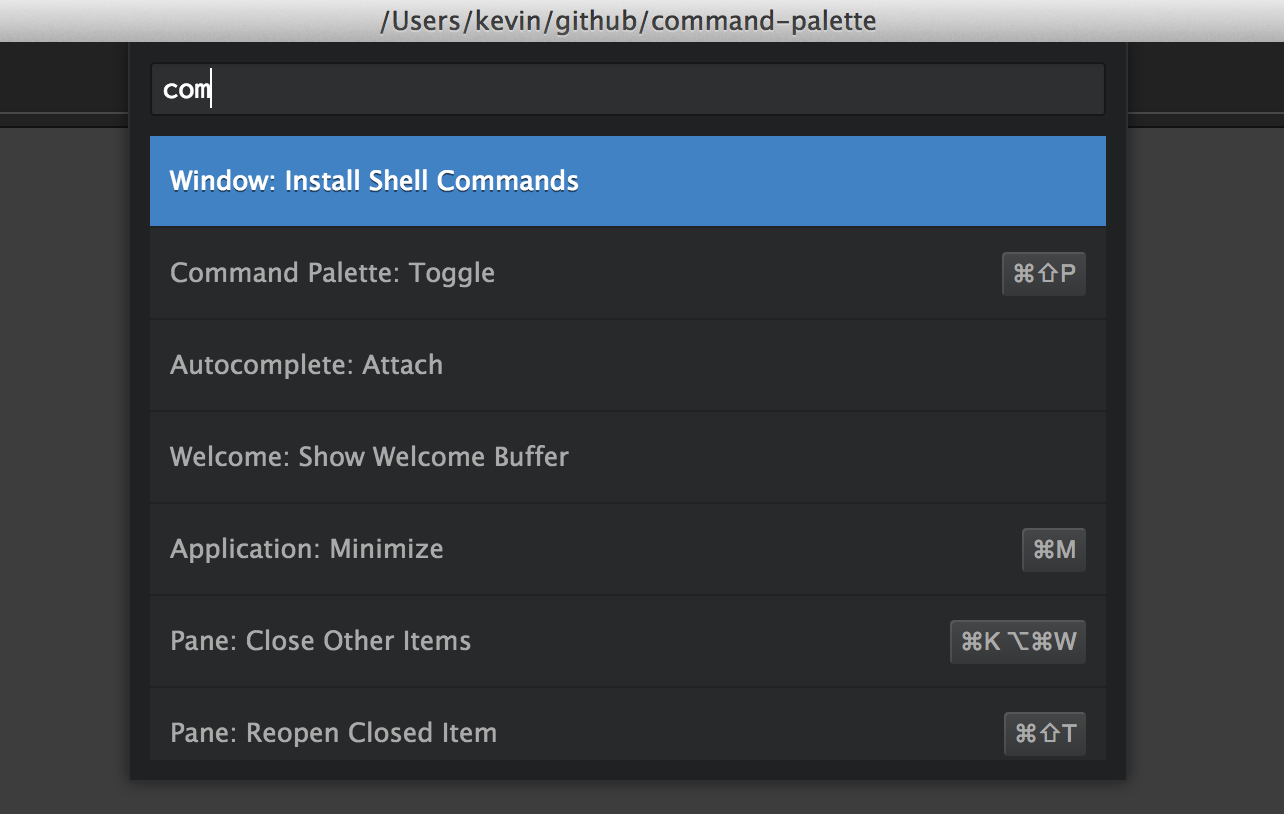
\includegraphics[scale=0.5]{atom_command_palette}
		\caption{Paleta komandi u programu Atom}
		\label{fig:atom_command_palette}
	\end{center}
\end{figure}

Paleta komandi (eng. \textit{command palette}) predstavlja listu dostupnih komandi koje se mogu izvr�iti unutar nekog programa i polje za unos klju�nih rije�i kako bi se brzo prona�la �eljena komande. Na slici \ref{fig:atom_command_palette} \cite{1_2019} prikazan je mogu�i izgled palete u programu \textit{Atom} (ure�iva� teksta i programskog koda) kada se unese "com". Korisnik mo�e odabrati i izvr�iti jednu od ponu�enih komandi. Paleta se poziva kori�tenjem tipkovni�kog pre�aca \textit{Cmd+Shift+P} na MacOS, odnosno \textit{Ctrl+Shift+P} na Linux i Windows operacijskim sustavima.

Dodatna prednost palete komandi je smanjivanje potrebe za prebacivanjem izme�u tipkovnice i mi�a (eng. \textit{homing} - prebacivanje s jednog na drugi ure�aj za upravljanje ra�unalom). U ovom radu implementirana je univerzalna paleta komandi, koja se mo�e koristiti u bilo kojem programu jer mo�e prepoznati aplikaciju koja se trenutno upotrebljava.

\section{Evaluacija univerzalne palete komandi}

Upotrebljivost univerzalne palete komandi ispituje se na temelju unaprijed definiranih zadataka koji uklju�uju rad s popularnim programima:

\begin{itemize}
	\item \textbf{Google Chrome} - web preglednik
	\item \textbf{LibreOffice Writer} - ure�iva� teksta
	\item \textbf{GIMP} - ure�iva� slika
\end{itemize}

Zadaci su osmi�ljeni tako da predstavljaju uobi�ajeni, svakodnevni rad na ra�unalu. Sastoje se od kombinacije �e��e i rje�e kori�tenih funkcionalnosti navedenih programa. Uspore�uje se vrijeme potrebno za obavljanje svih zadataka sa i bez univerzalne palete komandi na raspolaganju. Tako�er, preko predispitnih i postispitnih anketa �eli se dobiti uvid u kojoj mjeri ispitanici koriste tipkovni�ke pre�ace i palete komandi iz programa koji ih podr�avaju te na kraju njihovo zadovoljstvo s univerzalnom paletom komandi.
\chapter{Povezani i sli�ni radovi}

Osim paleta komandi prisutnih u ure�iva�ima programskog koda kao �to su \textit{Atom}, \textit{Sublime Text} i \textit{Visual Studio Code}, postoje i ostali sli�ni primjeri koji za cilj imaju olak�anu pretragu za naredbama neke aplikacije ili ubrzavanje rada s ra�unalom na neki drugi na�in.

\section{Unity HUD, Plotinus i Gnome HUD}

\begin{figure}[!htbp]
	\begin{center}
		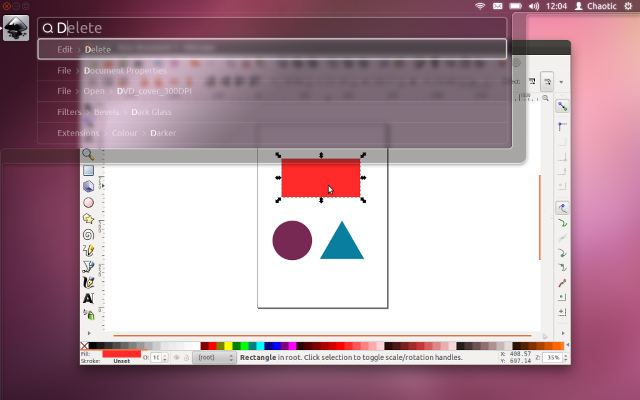
\includegraphics[scale=0.7]{unity_hud}
		\caption{Unity HUD \cite{11_2019}}
		\label{fig:unity_hud}
	\end{center}
\end{figure}

Kao proizvod koji je najsli�niji univerzalnoj paleti komandi isti�e se \textbf{Unity HUD} \cite{11_2019}, prisutan u grafi�koj ljusci za Linux operacijske sustave \textbf{Unity}. Unity HUD mo�e raditi na vi�e razli�itih programa, odnosno nije eksplicitno implementiran za to�no odre�ene aplikacije. Automatski u�itava naredbe iz izbornika programa koji je trenutno u fokusu te nudi mogu�nost njihovog pretra�ivanja i uporabe, �to se mo�e vidjeti na slici \ref{fig:unity_hud}. Unity HUD tako iskori�tava su�elje koje nude aplikacije na Linux sustavima iz kojih je mogu�e saznati stavke koje se nalaze u njihovim izbornicima.

Me�utim, ovaj program ima sljede�e nedostatke:

\begin{itemize}
\item Zbog na�ina implementacije ne mo�e se koristiti na Windows operacijskim sustavima (usko je vezan uz arhitekturu Linux aplikacija)
\item Unity ljuska za GNOME nije vi�e u aktivnom razvoju od strane autora iz tvrtke Canonical \cite{12_2019}
\end{itemize}

\begin{figure}[!htbp]
	\begin{center}
		\includegraphics[scale=0.7]{Plotinus}
		\caption{Plotinus \cite{13_2019}}
		\label{fig:plotinus}
	\end{center}
\end{figure}

Sli�no rje�enje je i \textbf{Plotinus}, vidljivo na slici \ref{fig:plotinus} koje, uz �injenicu da nije u aktivnom razvoju (zadnje osvje�enje je bilo 4.6.2017. godine), tra�i i ru�nu konfiguraciju odre�enih sistemskih datoteka, �to predstavlja prepreku za korisnike koji nemaju tehni�ka znanja za rad u Linux sustavima. Tako�er, kao i u slu�aju Unity HUD-a, Plotinus mo�e biti kori�ten samo na Linuxu.

\begin{figure}[!htbp]
	\begin{center}
		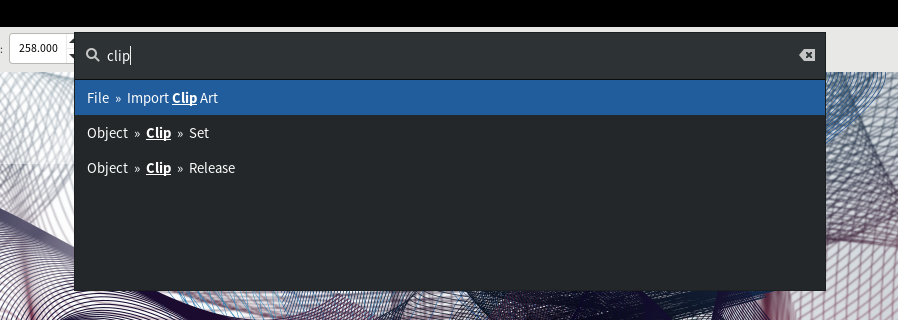
\includegraphics[scale=1.95]{gnome_hud}
		\caption{Gnome HUD \cite{14_2019}}
		\label{fig:gnome_hud}
	\end{center}
\end{figure}

Naposljetku, Gnome HUD, prikazan na slici \ref{fig:gnome_hud} se redovitije osvje�ava i tra�i manje konfiguracije, no svejedno je potrebno instalirati dodatne pakete za potpunu kompatibilnost s GTK i Qt alatima za izradu grafi�kih su�elja.

\section{Microsoft Office Tell Me}

\begin{figure}[!htbp]
	\begin{center}
		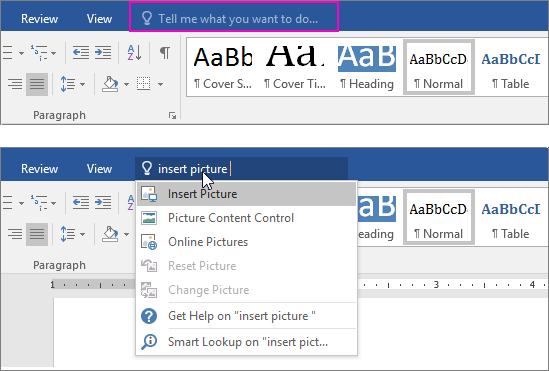
\includegraphics[scale=0.85]{microsoft_office_tell_me}
		\caption{Tell Me \cite{15_2019} u programu Microsoft Word}
		\label{fig:microsoft_office_tell_me}
	\end{center}
\end{figure}

U sklopu Microsoft Office paketa programa mo�e se na�i funkcionalnost naziva \textit{Tell Me}, odnosno punog naziva \textit{Tell me what you want to do} koja je prikazana na slici \ref{fig:microsoft_office_tell_me}. Njeno kori�tenje je iznimno jednostavno i intuitivno jer je dovoljno upisati naziv �eljene radnje i izbornik �e ponuditi naredbu koja je ina�e dostupna iz izbornika aplikacije.

Me�utim, ovo rje�enje je integrirano u Microsoft Office programe i nije primjenjivo na ostale aplikacije, �to je osnovna motivacija univerzalne palete komandi. No, ono predstavlja �elju da se rad sa slo�enim aplikacijama s mnogo mogu�nosti, kao �to su Microsoft Word ili PowerPoint, u�ini pristupa�nijim.


\chapter{Realizacija univerzalne palete komandi}

U ovom poglavlju bit �e opisan postupak dizajna i implementacije univerzalne palete komandi, �to uklju�uje inicijalni dizajn su�elja i korisni�kog iskustva, izbora alata za samu implementaciju te kona�ni izgled same aplikacije. Na kraju poglavlja su opisani razni izazovi vezani uz implementaciju te prijedlozi za mogu�a pobolj�anja palete.

\section{Dizajn}

Na slici \ref{fig:snv_design} prikazan je �eljeni izgled univerzalne palete komandi koji se sastoji od dvije osnovne cjeline: polja za unos teksta i liste komandi. Pritom, maksimalni broj vidljivih komandi u listi �e se mo�i mijenjati (po�etna postavka je deset komandi). Ukoliko se u listi komandi nalazi vi�e stavki od tog broja, pojavljuje se vertikalna traka za pomicanje (engl. \textit{scrollbar}) kako bi korisnici mogli imati pristup svim komandama. Uvijek je ozna�ena samo jedna komanda a unosom odre�enog pojma prikazuje se lista koja odgovara tom pojmu.

\begin{figure}[!htbp]
	\begin{center}
		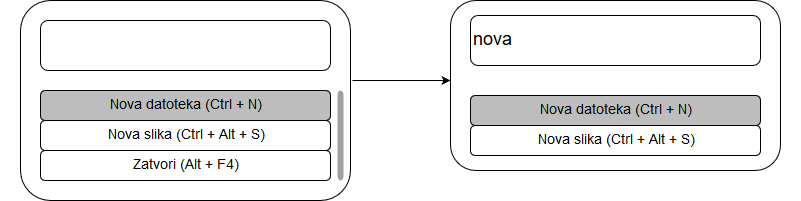
\includegraphics[scale=0.70]{snv_design}
		\caption{Skica �eljenog izgleda univerzalne palete komandi}
		\label{fig:snv_design}
	\end{center}
\end{figure}

Paletom �e se mo�i upravljati s tipkovnicom (koriste�i strelice za gore i dolje te \textit{Enter} za odabir komande) ili s mi�em (kori�tenjem trake za pomicanje i klikanjem na �eljenu komandu).

\begin{figure}[!htbp]
	\begin{center}
		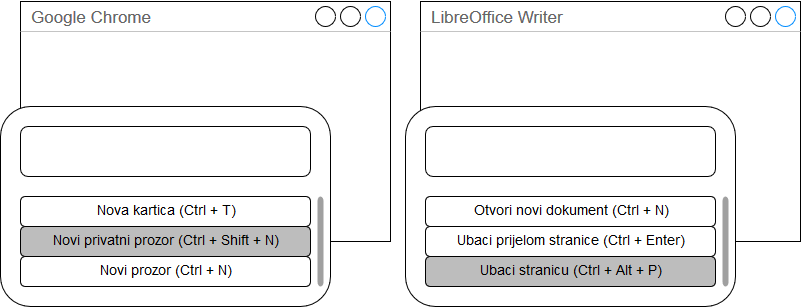
\includegraphics[scale=0.70]{snv_app_aware}
		\caption{Univerzalna paleta komandi je svjesna aplikacije koju korisnik trenutno upotrebljava}
		\label{fig:snv_app_aware}
	\end{center}
\end{figure}

Glavna zna�ajka univerzalne palete komandi je njena svjesnost o aplikaciji koju korisnik trenutno upotrebljava, �to je vidljivo na slici \ref{fig:snv_app_aware} (prikazane komande su samo za demonstraciju koncepta). Ovisno o aplikaciji, izbor komandi se razlikuje.

Dodatno, univerzalna paleta komandi �e pamtiti i frekvenciju kori�tenja svake komande, kako bi one koje se naj�e��e koriste bile prikazane na vrhu liste. Nakon iznesenih zahtjeva, name�u se sljede�i izazovi:
\begin{itemize}
	\item Kako prepoznati aplikaciju koja se trenutno koristi?
	\item Koji je univerzalan na�in na koji neki program mo�e izvr�iti bilo koju radnju u nekom drugom programu?
\end{itemize}

Prvi problem je rije�en tako da se koristi alat za prepoznavanje procesa kojem trenutno fokusirani prozor pripada te se u skladu s time u�itava odgovaraju�a lista komandi. Kod drugog izazova, izvr�avanje komandi se posti�e emulacijom tipkovni�kih pre�aca. Primjerice, kod izvr�avanja komande "\textit{Otvori datoteku"}, univerzalna paleta �e emulirati tipkovni�ki pre�ac "\textit{Ctrl + O}".

Tipkovni�ki pre�aci su koncept koji je �iroko rasprostranjen u programskoj potpori na klasi�nim, \textit{desktop} ra�unalima, gdje se koriste mi� i tipkovnica. Zahtjevno je prona�i aplikaciju koja ih ne koristi kako bi svojim korisnicima omogu�ila ubrzani rad s aplikacijom. Zbog toga, emuliranje pre�aca, kao i svjesnost o aplikaciji koja je trenutno u fokusu, donosi \textbf{univerzalnost} ovom programu.

\section{Dijagram toka}

\begin{figure}[!htbp]
	\begin{center}
		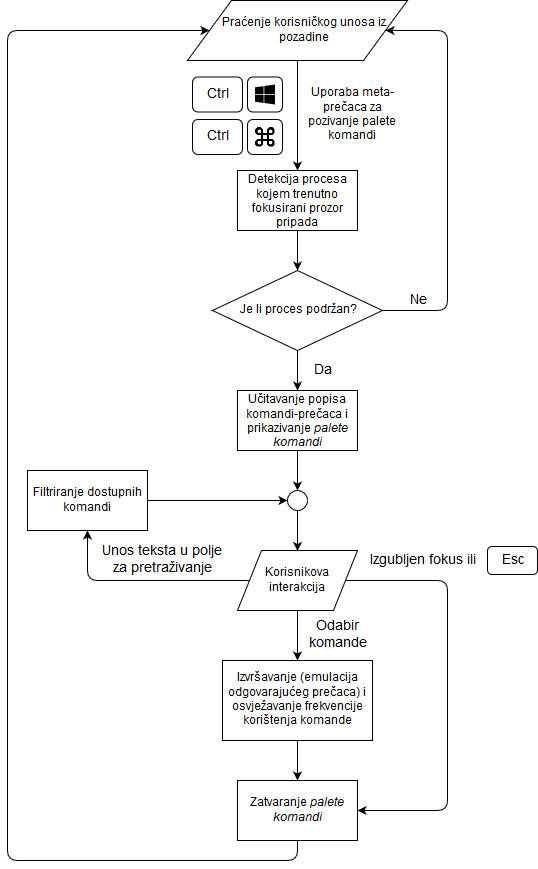
\includegraphics[height=17cm,width=17cm,keepaspectratio=true]{snv_flow_diagram}
		\caption{Dijagram toka rada univerzalne palete komandi}
		\label{fig:snv_flow_diagram}
	\end{center}
\end{figure}

Cjelokupni na�in rada univerzalne palete komandi prikazan je na slici \ref{fig:snv_flow_diagram}. Ve�inu vremena, ovaj program �e provesti kao pozadinski proces (engl. \textit{daemon}) te �e oslu�kivati korisnikove unose na tipkovnici. U trenutku kada korisnik upotrijebi \textit{meta-pre�ac}, koji je u ovom radu pode�en na \textit{Ctrl + Win}, program �e provjeriti prvo je li aplikacija koja se trenutno koristi podr�ana. Ako nije, ne�e se ni�ta dogoditi, a u suprotnom slu�aju, u�itat �e se lista komandi i paleta �e se prikazati na ekranu.

Korisnik mo�e pretra�iti i izvr�iti �eljenu komandu ili mo�e zatvoriti paletu pritiskom na tipku \textit{Esc} ili gubitkom fokusa na paletu (klikom izvan njenog prozora).

\section{Implementacija}

Prototip univerzalne palete komandi u po�etku izrade ovog rada implementiran je za sustave zasnovane na Linuxu. Konkretno, koristila se Antergos distribucija s \textbf{KDE} okru�enjem. Prototip se temelji na programskom jeziku Python 3.7.2 i sljede�im modulima:

\begin{itemize}
	\item \textit{Tkinter} je \textit{de-facto} standardni paket za razvoj GUI aplikacija, temeljen na \textbf{Tcl/Tk} alatima \cite{2_2019}. Slu�i za implementaciju korisni�kog su�elja univerzalne palete komandi.
	\item \textit{PyAutoGUI} je modul za programsko izvr�avanje (emulaciju) uporabe mi�a i tipkovnice. Koristi se za emulaciju tipkovni�kih pre�aca, �ime univerzalna paleta komandi mo�e izvr�iti neku radnju u bilo kojoj drugoj aplikaciji.
	\item \textit{Pynput} je knji�nica funkcija za oslu�kivanje korisnikovog unosa na tipkovnici. Omogu�ava uporabu meta-pre�aca za pozivanje univerzalne palete komandi.
\end{itemize}

Za prepoznavanje aplikacije koju korisnik trenutno upotrebljava koristi se Linux alat \textit{xdotool} \cite{3_2019}, uz �iju se pomo� mo�e saznati PID (engl. \textit{Process ID}) trenutno kori�tene aplikacije. S tom informacijom, od poznate \textit{shell} naredbe \textit{ps} mogu�e je saznati ime procesa s tim PID-om.

Komande se spremaju kao JSON datoteke zasebno za svaku aplikaciju. Nazivi tih datoteka odgovaraju imenima procesa tih aplikacija u Linux sustavima.

\begin{figure}[!htbp]
	\begin{lstlisting}[language=json, label={code:2.1}, caption={Pokazni primjer mogu�e JSON datoteke za konfiguraciju komandi u programu Google Chrome}]
{
   "Bookmark": {
      "type": "shortcut",
      "shortcuts": [
         [
         "ctrl",
         "d"
         ]
      ],
      "frequency": 0
   },
   "Clear Browsing Data": {
      "type": "shortcut",
      "shortcuts": [
         [
            "ctrl",
            "shift",
            "del"
         ]
      ],
      "frequency": 0
   }
}
	\end{lstlisting}
\end{figure}

U isje�ku koda \ref{code:2.1} mo�emo vidjeti kako bi izgledao JSON zapis komandi za program Google Chrome kada bismo imali samo dvije stavke. Pri tome, va�no je napomenuti da oznake za tipke koje �ine odre�eni tipkovni�ki pre�ac (\textit{ctrl}, \textit{shift}, \textit{del} i sli�ni) moraju odgovarati oznakama koje se pojavljuju u dokumentaciji za modul \textit{PyAutoGUI} \cite{4_2019}.

Prvo polje (u ovom primjeru \textit{Bookmark} i \textit{Clear Browsing Data}) predstavlja ime komande, odnosno ono �to �e se korisniku univerzalne palete komandi prikazati na ekranu.

Polje \textit{frequency} ozna�ava koliko je puta komanda bila kori�tena otkad je korisnik po�eo upotrebljavati univerzalnu paletu komandi.

JSON predstavlja prikladan format za zapis podataka ovakvog oblika jer je jednostavan za uporabu i �itljiv ljudima (engl. \textit{human-readable}).

\section{Prezentacija}

\begin{figure}[!htpb]
	\begin{center}
		\subfloat[Bez unosa]{\label{fig:aacp_before} 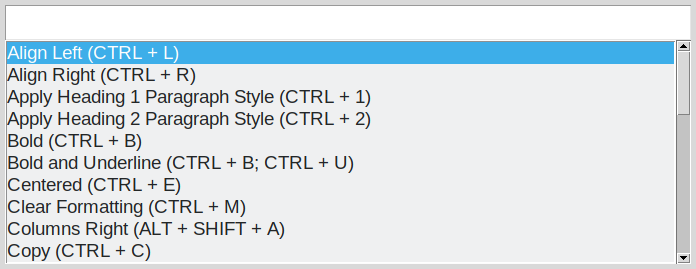
\includegraphics[scale=0.75]{aacp_before}} \\
		\subfloat[S unosom]{\label{fig:aacp_after} 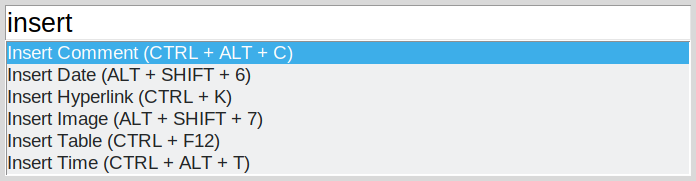
\includegraphics[scale=0.75]{aacp_after}}
		\caption{Kona�ni izgled univerzalne palete komandi}
		\label{fig:aacp_look}
	\end{center}
\end{figure}

Kona�ni izgled prototipa univerzalne palete komandi prikazan je na slici \ref{fig:aacp_look}. Svaka komanda pored svog naziva ima i odgovaraju�i pre�ac, �to korisniku mo�e pomo�i da kroz rad upamti nove pre�ace te ih s vremenom po�ne i koristiti, kako bi u kra�em roku dolazio do funkcionalnosti koje mu trebaju.

Glavni jezik programa je engleski, jer je pretpostavka da �e ispitanici biti bolje upoznati s radom u programskoj potpori koja je pode�ena za originalni, engleski jezik.

\begin{figure}[!htpb]
	\begin{center}
		\subfloat[Google Chrome]{\label{fig:aacp_chrome} 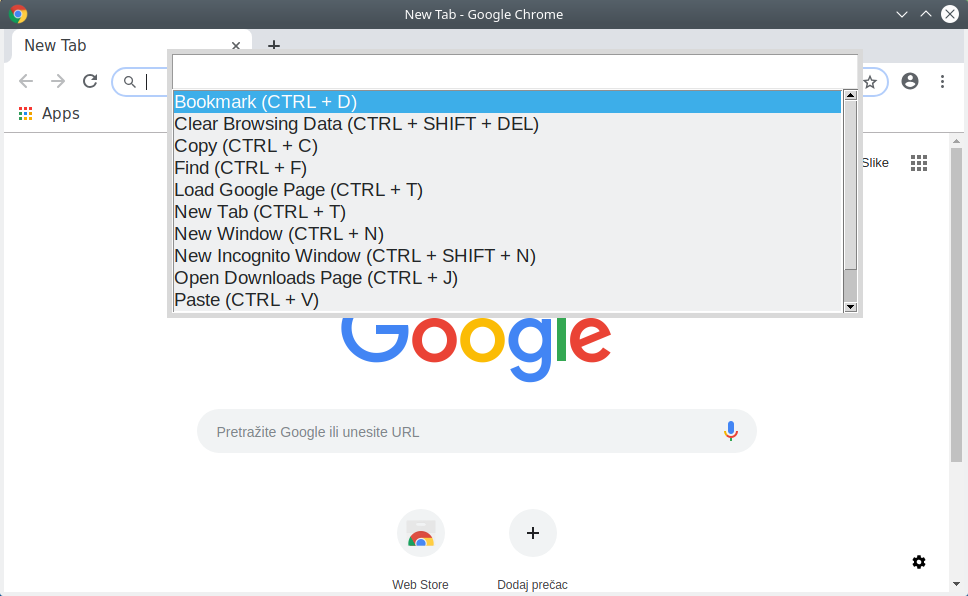
\includegraphics[scale=0.55]{aacp_chrome}} \\
		\subfloat[LibreOffice Writer]{\label{fig:aacp_office} 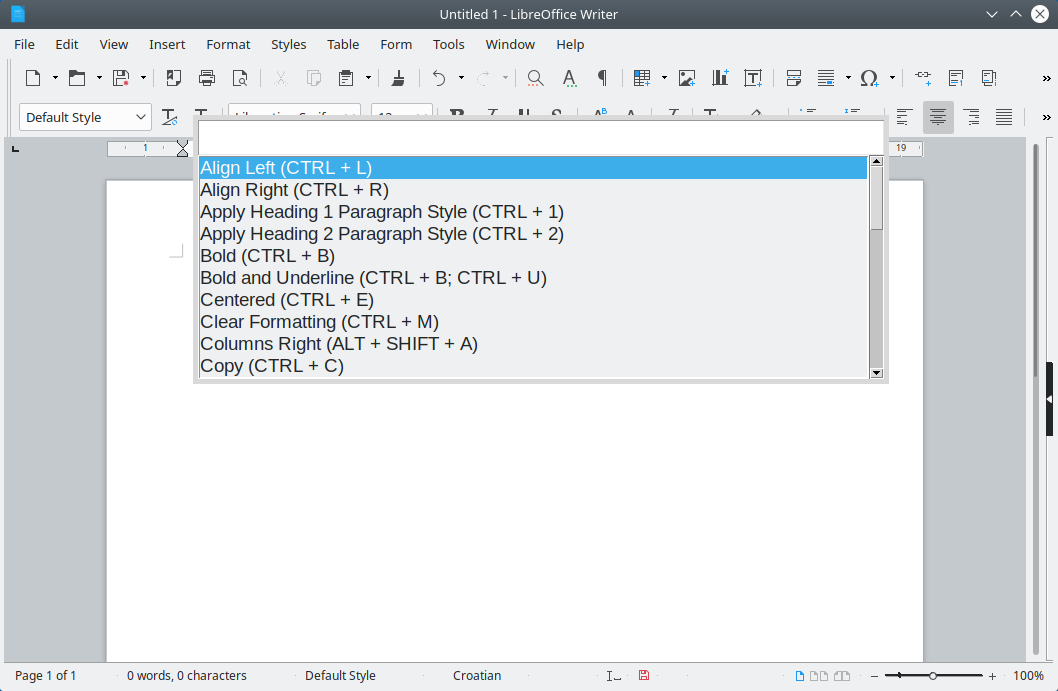
\includegraphics[scale=0.5]{aacp_office}}
		\caption{Paleta komandi je svjesna aplikacije za koju se trenutno koristi}
		\label{fig:aacp_app_aware}
	\end{center}
\end{figure}

Slika \ref{fig:aacp_app_aware} prikazuje stvarne primjere prilagodljivosti univerzalne palete komandi. Ovisno o aplikaciji kojoj pripada prozor koji je trenutno u fokusu, bit �e ponu�ene razli�ite komande, odnosno one koje odgovaraju toj aplikaciji. Paleta na taj na�in predstavlja jedinstveno su�elje koje se mo�e koristiti u mnogo razli�itih konteksta.

\begin{figure}[!htbp]
	\begin{center}
		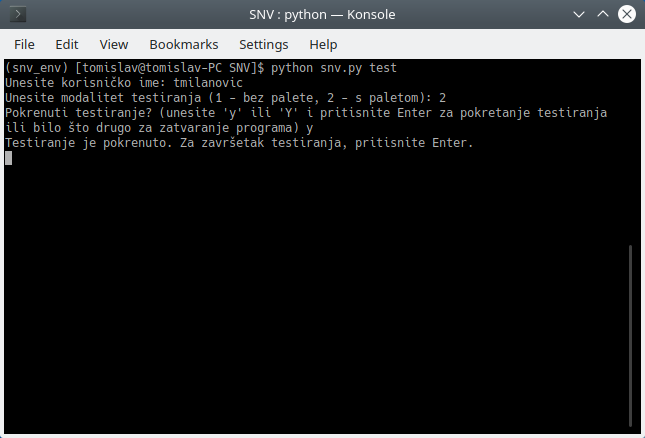
\includegraphics[scale=0.70]{aacp_test}
		\caption{Testni na�in rada}
		\label{fig:aacp_test}
	\end{center}
\end{figure}

Dodatno, u svrhu provo�enja eksperimenta i ispitivanja upotrebljivosti univerzalne palete komandi uveden je i \textbf{testni na�in rada}, �to se mo�e vidjeti na slici \ref{fig:aacp_test}. Predvi�ena su dva modaliteta testiranja. U jednom modalitetu kori�tenje palete je dano na raspolaganje a u drugom nije (ovdje se program pokre�e samo za svrhu mjerenja vremena obavljanja ispitnog zadatka).

Nakon zavr�etka testiranja (pritiskom na tipku \textit{Enter}) stvorit �e se tekstualna datoteka s imenom oblika \textit{korisnickoime\_modalitet\_report.txt}. Primjer jedne takve datoteke izgleda kao �to je prikazano u nastavku:

\begin{verbatim}
Username: tmilanovic
Start Timestamp: 1358.316003
	
Commands:
soffice.bin: Align Left - 1365.989010
soffice.bin: Apply Heading 2 Paragraph Style - 1367.789081
soffice.bin: Find and Replace - 1370.069251
	
End Timestamp: 1373.265085
	
Number of executed commands: 3
Measured time: 14.949082 s
\end{verbatim}

Ovdje se nalazi popis svih komandi koje su bile upotrijebljene za vrijeme testiranja (ime Linux procesa za kojeg su bile iskori�tene, njihovo ime i vremenski trenutak u kojem su izvr�ene).

Vremenske pe�ate (engl. \textit{timestamps}) ispisuje Python metoda \textit{time.monotonic()} \cite{5_2019}. Definirani su u sekundama i nemaju referentnu to�ku ve� je potrebno promatrati razliku izme�u dva pe�ata za mjerenje vremena. Glavna karakteristika \textit{monotonic} satova je da na njih ne utje�e promjena sistemskog sata.

Izvje�taj za prvi modalitet rada (bez palete) razlikuje se u izostanku popisa komandi.

\section{Implementacija Windows verzije}

Budu�i da univerzalna paleta komandi nastoji posti�i visoku razinu kompatibilnosti i s razli�itim operacijskim sustavima koji se koriste na klasi�nim, stolnim ra�unalima, implementiran je i prototip verzije za operacijski sustav Windows.

\begin{figure}[!htbp]
	\begin{python}[label={code:2.3}, caption={Prepoznavanje procesa kojem pripada trenutno fokusirani prozor u operacijskim sustavima Windows}]
import os
import win32gui
import win32process
import psutil
	
def get_process_name_windows():
 try:
   w_gui = win32gui
   w_process = win32process
   foreground_window = w_gui.GetForegroundWindow()
   pid = w_process.GetWindowThreadProcessId(foreground_window)
   process_name = psutil.Process(pid[-1]).name()
  except:
   process_name = ''

  process_name = os.path.splitext(process_name)[0]
  return process_name
	\end{python}
\end{figure}

Implementiranje podr�ke za Windows sustave iziskivalo je nadogradnju trenutnog programskog koda palete. Bilo je potrebno rije�iti dva osnovna problema. Prvi problem je �injenica da se \textit{xdotool}, koji na Linux sustavima omogu�ava detekciju procesa kojem pripada trenutno fokusirani prozor, ne mo�e upotrebljavati na operacijskim sustavima Windows. Zbog toga se zajedno koriste \textit{Win32 API} za Python \cite{7_2019} i \textit{psutil} modul \cite{8_2019} kako bi se doznalo ime procesa (izvr�ne datoteke) na temelju �ega se u�itava odgovaraju�a JSON datoteka, �to je prikazano u isje�ku koda \ref{code:2.3}.

Drugi glavni izazov je �injenica da Windows ima stroge kriterije dozvoljavanja aplikaciji da sama programski poku�a postati glavni, fokusirani prozor \cite{9_2019}. Razlog tome je �elja da se korisniku ne name�e neki prozor dok ga on sam eksplicitno ne fokusira. Me�utim, budu�i da korisnik itekako samostalno izra�ava �elju za pozivanjem univerzalne palete komandi, koja se cijelo vrijeme izvr�ava kao pozadinski proces, te u skladu s time nije trenutno aktivni prozor, potrebno je osmisliti na�in kako da paleta mo�e postaviti fokus na sebe. Tako�er, nakon �to se paleta zatvori zbog izvr�avanja izabrane komande, fokus se ne vra�a automatski na prozor aplikacije za koju je korisnik pozvao paletu.

\begin{figure}[!htbp]
	\begin{python}[label={code:2.4}, caption={Postavljanje fokusa na prozor palete}]
w = win32gui
# Pam�enje prozora trenutno kori�tene aplikacije
currentApp = w.GetForegroundWindow()
...
import ctypes
set_to_foreground = ctypes.windll.user32.SetForegroundWindow
keybd_event = ctypes.windll.user32.keybd_event
alt_key = 0x12
extended_key = 0x0001
key_up = 0x0002

def steal_focus():
    # Emulacija pritiska tipke 'alt', �to omogu�ava postavljanje fokusa na paletu
    keybd_event(alt_key, 0, extended_key | 0, 0)
    set_to_foreground(root.winfo_id())
    keybd_event(alt_key, 0, extended_key | key_up, 0)
    ...
    entry.focus_force()

def bind_focus_out():
    mainframe.bind('<FocusOut>', gui_close)
# Postavljanje fokusa 200 ms nakon pozivanja palete
root.after(200, steal_focus)
# Povezivanje metode za zatvaranje prozora nakon 500 ms
# Ovo je uvedeno zato jer se prozor palete brzo zatvara 
# nakon pozivanja
root.after(500, bind_focus_out)
...
def gui_close(entry=""):
   	...
    # Vra�anje fokusa na prija�nju aplikaciju
    win32gui.SetForegroundWindow(currentApp)
	\end{python}
\end{figure}

\begin{figure}[!htp]
	\begin{center}
		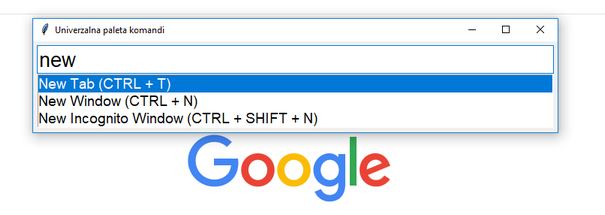
\includegraphics[scale=0.53]{aacp_windows}
		\caption{Windows ina�ica prototipa univerzalne palete komandi}
		\label{fig:aacp_windows}
	\end{center}
\end{figure}

Rje�enje problema fokusa prikazano je u isje�ku koda \ref{code:2.4}. Rje�enje se temelji na odgovoru \cite{10_2019}, odnosno na emulaciji pritiska tipke \textbf{Alt} �to omogu�uje postavljanje fokusa na �eljeni prozor. Kona�no, izgled same palete, u kontekstu programa \textit{Google Chrome} kad se koristi na operacijskom sustavu Windows, mo�e se vidjeti na slici \ref{fig:aacp_windows}.

\section{Izazovi i mogu�a pobolj�anja} \label{sec:challenges}

\subsection{Izazovi podr�ke funkcionalnostima}

Nisu sve funkcionalnosti koje se mogu koristiti u nekoj aplikaciji pokrivene odgovaraju�im tipkovni�kim pre�acem. Me�utim, programi u svojim postavkama �esto imaju mogu�nost prilagodbe tipkovni�kih pre�aca za one funkcionalnosti koje ga ina�e nemaju. Na taj na�in mo�e se ostvariti pro�irenje opsega funkcionalnosti koje se mogu izvr�iti uz pomo� univerzalne palete komandi. Dodatna prednost kod takvih programa bila bi mogu�nost spremanja postavki tipkovni�kih pre�aca u datoteke koje se zatim mogu dijeliti sa zajednicom korisnika tog programa.

Programi �esto sadr�avaju mnogobrojne funkcionalnosti i mogu�nosti, �to zna�i da izrada JSON datoteke za univerzalnu paletu komandi mo�e iziskivati odre�eno vrijeme i trud. Sre�om, tu je datoteku dovoljno napisati samo jednom, a zatim se ona mo�e dijeliti unutar potencijalne zajednice korisnika univerzalne palete komandi. Kako bi proces pisanja JSON datoteke bio pristupa�an korisnicima (engl. \textit{user friendly}), postoji opcija izrade aplikacije koja bi slu�ila ure�ivanju takvih datoteka, bez potrebe da se direktno ure�uje JSON zapis za njih u jednom od ure�iva�a teksta.

\subsection{Izazovi ispravne detekcije programa}

Prema iznesenom dizajnu univerzalne palete komandi, detekcija aplikacije koju korisnik trenutno upotrebljava vr�i se uz pomo� imena procesa u Linux sustavu ili imena izvr�ne datoteke u Windows sustavima. Tijekom implementacije podr�ke za \textit{LibreOffice Writer} uo�eno je da svi programi u \textit{LibreOffice} softverskom paketu imaju identi�no ime procesa: \textit{soffice.bin}. To predstavlja problem prilikom u�itavanja odgovaraju�e JSON datoteke ako se �eli ostvariti podr�ka za sve programe koji �ine taj paket.

Ovaj problem se mo�e rije�iti tako da se u razmatranje prilikom detekcije programa uzme i naslov prozora. Oni se prili�no razlikuju, naj�e��e sadr�avaju ime otvorene datoteke ili u slu�aju preglednika interneta i ime stranice koju korisnik trenutno pregledava. Va�no je u tom slu�aju programski obraditi taj naslov tako da se iz njega i��ita ime aplikacije, koje se naj�e��e nalazi na kraju naslova prozora.

Na kraju, treba uzeti u obzir i �injenicu kako se s vremenom pojavljuju nove verzije aplikacija, koje mogu imati nove funkcionalnosti i samim time potencijalne nove komande za paletu. U Linux sustavima se verzija �esto mo�e dobiti pokretanjem komande koja odgovara programu u konzoli s argumentom "-v" ili "-{}-version". U Windows sustavima se ta informacija mo�e dobiti iz izvr�nih datoteka programa.

Ako se do te informacije ne mo�e do�i programski, preostaje ponuditi korisniku izbor odgovaraju�e verzije preko postavki univerzalne palete.
\chapter{Eksperiment}

U cilju istra�ivanja potencijalnih prednosti i pozitivnih u�inaka koje bi uporaba univerzalne palete komandi mogla imati, proveden je eksperiment u kojem se ispitivalo kori�tenje palete u kontekstu svakodnevnog rada na tipi�nim GUI aplikacijama. Ciljana ispitna skupina su studenti i profesori ra�unarstva na Tehni�kom fakultetu u Rijeci, odnosno korisnici koji imaju iskustva rada na programima poput ure�iva�a teksta, internetskog preglednika i ure�iva�a slika.

Materijali kori�teni u samom ispitivanju (predispitne i postispitne ankete, suglasnost za testiranje korisnika i tekstovi zadatka) nalaze se u prilogu ovog rada.

\section{Suglasnost i predispitna anketa}

Na samom po�etku, ispitanicima je predstavljena suglasnost za testiranje (dodatak \ref{p:suglasnost} na stranici \pageref{p:suglasnost}), u kojoj su sljede�e tvrdnje najva�nije:

\begin{itemize}
\item sudjelovanje je dobrovoljno, mo�e se odustati u bilo kojem trenutku,
\item ispituje se univerzalna paleta komandi i njene mo�ebitne prednosti, a ne ispitanik,
\item ispitni koordinator �e uvijek biti prisutan i na raspolaganju za sva pitanja,
\item podaci dobiveni prilikom testiranja pripadaju fakultetu,
\item imena i prezimena ispitanika \textbf{ne�e} biti objavljena ni u kakvom znanstvenom radu, ve� samo podaci dobiveni kroz ispitivanje
\end{itemize}

Nakon suglasnosti, ispitanici su trebali ispuniti predispitnu anketu (dodatak \ref{p:predispitna} na stranici \pageref{p:predispitna}). Na prvoj stranici ankete ispituje se u�estalost i iskustvo kori�tenja tipkovni�kih pre�aca (eng. \textit{keyboard shortcuts}) ili nekih drugih alata, metoda i ostalog �to se razlikuje od uobi�ajenog kori�tenja ra�unala (prolasci po izbornicima, alatnoj traci i sli�no) a slu�i unapre�enju rada na ra�unalu tako �to omogu�uje brzi pristup raznim funkcionalnostima aplikacije koja se koristi. Tako�er, ispituje se iskustvo rada u tri glavne vrste aplikacija koje se pojavljuju u samom zadatku eksperimenta: ure�iva� teksta, internetski preglednik i ure�iva� slika.

Na drugoj stranici ispituje se prethodno znanje nekoliko tipkovni�kih pre�aca aplikacija koje se pojavljuju u ispitnom zadatku (LibreOffice Writer, Google Chrome i Gimp). Ovdje se nalaze uobi�ajene funkcionalnosti, kao �to su, izme�u ostalog, \textit{Kopiraj}, \textit{Zalijepi}, \textit{Otvori datoteku}, \textit{Naslov druge razine} i \textit{Umetni tablicu}. Identi�na pitanja pojavljuju se i u postispitnoj anketi. Ukratko, cilj ove ankete je dobiti uvid u to koliko je univerzalna paleta komandi ispitanicima pomogla zapamtiti tipkovni�ke pre�ace za navedene funkcionalnosti (jer se ti tipkovni�ki pre�aci nalaze u zagradama desno od komandi u samoj paleti). Ispitanicima je poja�njen smisao ove ankete prije nego �to krenu rje�avati zadatak eksperimenta.

\section{Demonstracija palete komandi i ispitni zadatak}

Prije rje�avanja samog zadatka, ispitanicima je odr�avana kratka demonstracija univerzalne palete komandi. Nagla�eno im je da pretra�uju po rije�i koja najbolje opisuje funkcionalnost. Primjerice, ukoliko trebaju umetnuti sliku u dokument, u polje za unos teksta trebaju upisati \textit{image} (slika) a ne \textit{insert} (umetni) jer �e tako br�e do�i do �eljenog pojma. Drugo, napomenuto im je da paleta slu�i kao ispomo�, odnosno dodatni alat koji je na raspolaganju, ali da ju ne moraju koristiti za obavljanje svake radnje, ve� samo kada osobno smatraju da bi im ubrzao rad i smanjio trud za pronalaskom tra�ene funkcionalnosti. Ukratko, mogli su ga koristiti po vlastitoj slobodnoj volji. Na kraju demonstracije, ispitanicima je omogu�ena proba same palete, kako bi ju nau�ili koristiti.

\begin{table}[!htbp]
\caption{Raspored jedinstvenih komandi ovisno o tome imaju li standardni ili ru�no pode�eni tipkovni�ki pre�ac}
\centering
\begin{tabular}{|l|c|c|c|}
\hline
Vrsta komande & \multicolumn{1}{l|}{Google Chrome} & \multicolumn{1}{l|}{Gimp} & \multicolumn{1}{l|}{LibreOffice Writer} \\ \hline
nativna       & 4                                  & 2                         & 6                                       \\ \hline
umjetna       & 0                                  & 2                         & 10                                      \\ \hline
\end{tabular}
\label{tab:commands}
\end{table}

Nakon demonstracije, ispitanici su trebali pro�itati barem tri podzadatka, kako bi stekli dojam o cjelokupnom zadatku prije nego �to ga krenu rje�avati. Sam ispitni zadatak (dodatak \ref{p:eksperimentalni} na stranici \pageref{p:eksperimentalni}) se sastoji od 13 podzadataka i 24 jedinstvenih komandi koje se mogu izvr�iti uz pomo� univerzalne palete. Niti jedna komanda se ne ponavlja. U tablici \ref{tab:commands} mo�emo vidjeti raspored tih jedinstvenih komandi ovisno o tome dolaze li s ve� pode�enim tipkovni�kim pre�acem ili ga je potrebno ru�no konfigurirati. Kako je opisano u poglavlju 2, ukoliko neka funkcionalnost nema odgovaraju�i tipkovni�ki pre�ac, potrebno ga je podesiti u samom programu kako bi univerzalna paleta komandi mogla podr�avati tu funkcionalnost. Broj nativnih i umjetnih komandi je jednak.

Podzadaci unutar ispitnog zadatka predstavljaju tipi�ni, svakodevni rad na tri razli�ita programa - LibreOffice Writer, Google Chrome i Gimp. Cilj je opona�ati uobi�ajeni rad za ra�unalom, koji tako�er uklju�uje i u�estalo prebacivanje izme�u razli�itih aplikacija. Funkcionalnosti koje su izvr�ive uz pomo� univerzalne palete komandi su napisane u kurzivu s engleskim nazivom u zagradi. Sam eksperiment je u obliku \textbf{ponavljanog mjerenja} (eng. \textit{repeated measures}), gdje svi ispitanici trebaju pro�i zadatak kroz sljede�a dva modaliteta:

\begin{itemize}
\item bez univerzalne palete komandi - rije�iti zadatak na bilo koji na�in
\item s univerzalnom paletom komandi - rije�iti zadatak na bilo koji na�in uz paletu komandi na raspolaganju
\end{itemize}

Pogre�ke pri rje�avanju ispitnog zadatka se nisu mjerile niti bilje�ile. Jedine pogre�ke na kojima se inzistiralo da se isprave su preskakanje ili zaboravljanje izvr�avanja podzadataka, kako bi cijeli eksperiment bio u potpunosti odra�en. Pokraj ispitanika je cijelo vrijeme bio prisutan ispitni koordinator koji im je ukazivao na te pogre�ke ali i pru�ao pomo� kada je bilo potrebno.

Pri radu u prvom modalitetu, ukoliko korisnici ne bi unutar 30 sekundi prona�li tra�enu funkcionalnost, ispitni koordinator bi im pomogao u njenom tra�enju te bi na vlastiti papir (dodatak \ref{p:tablica} na stranici \pageref{p:tablica}) zapisao za koju radnju im je bila potrebna pomo�. Kako bi se sprije�io efekt nau�enosti na zadatke, primijenjena je metoda ravnote�e (eng. \textit{counterbalancing}) u dva aspekta:

\begin{itemize}
\item polovica ispitanika je u po�etku prolazila kroz prvi modalitet dok je druga polovica kretala s drugim modalitetom
\item postoje tri verzije ispitnog zadatka, koje se sastoje od identi�nih podzadataka, ali su oni u razli�itim redoslijedima
\end{itemize}

U ovom eksperimentu, nezavisna varijabla je modalitet interakcije (bez ili s paletom komandi) a zavisna varijabla je vrijeme potrebno za rje�avanje ispitnog zadatka.

Eksperiment se provodio na prijenosnom ra�unalu \textit{Acer Aspire F5-571G-38Y9} s \textit{Antergos} distribucijom Linuxa i \textit{KDE Plasma 5} radnim okoli�em. Ra�unalo se nalazilo desno od monitora na kojeg je bilo spojeno. Na monitoru su sudionici rje�avali zadatak, dok je na ekranu samog ra�unala bio prikazan tekst ispitnog zadatka. Ispitanici su tako�er imali na raspolaganju standardni mi� i tipkovnicu te im je bilo preporu�eno da ne koriste dodirnu plo�icu i tipkovnicu samog prijenosnog ra�unala.

Svako ispitivanje je bilo odra�eno u prostoriji 1-40 (SEIP Lab) na Tehni�kom fakultetu u Rijeci. Ispitanici su imali mir koji je bio nu�an za kvalitetno i koncentrirano rje�avanje ispitnog zadatka.

\section{Postispitna anketa i zavr�etak eksperimenta}

Jedan od ciljeva postispitne ankete je saznati kakav su dojam ispitanici stekli o univerzalnoj paleti komandi nakon rje�avanja ispitnog zadatka (dodatak \ref{p:postispitna} na stranici \pageref{p:postispitna}). U tu svrhu, koristio se popularni SUS \cite{6_2019} (eng. \textit{System Usability Score}) upitnik. Rje�avanjem standardiziranih pitanja, ispitanici su iskazivali svoje mi�ljenje o prototipu koji im je bio prezentiran.

Na samom kraju, ponovljena je anketa o znanju tipkovni�kih pre�aca aplikacija u kojima se rje�avao ispitni zadatak. Zaklju�no, cjelokupni eksperiment, zajedno s anketama, demonstracijama, rje�avanjem ispitnog zadatka, pauzama i neformalnim razgovorima imao je po sudioniku prosje�no trajanje od 30 do 40 minuta.
\chapter{Rezultati istra�ivanja}

U ovom poglavlju bit �e opisani rezultati dobiveni nakon provedenog istra�ivanja. U njemu je sudjelovalo ukupno trideset ispitanika (23 mu�karaca i 7 �ena) �ija je dob bila u rasponu od 21 do 40 godine, s prosjekom od 23,5 godina. Svi ispitanici su, kako je bilo planirano, studenti ra�unarstva ili profesori sa Zavoda za ra�unarstvo na Tehni�kom fakultetu u Rijeci.

\section{Rezultati predispitne ankete}

\begin{figure}[!htbp]
	\begin{center}
		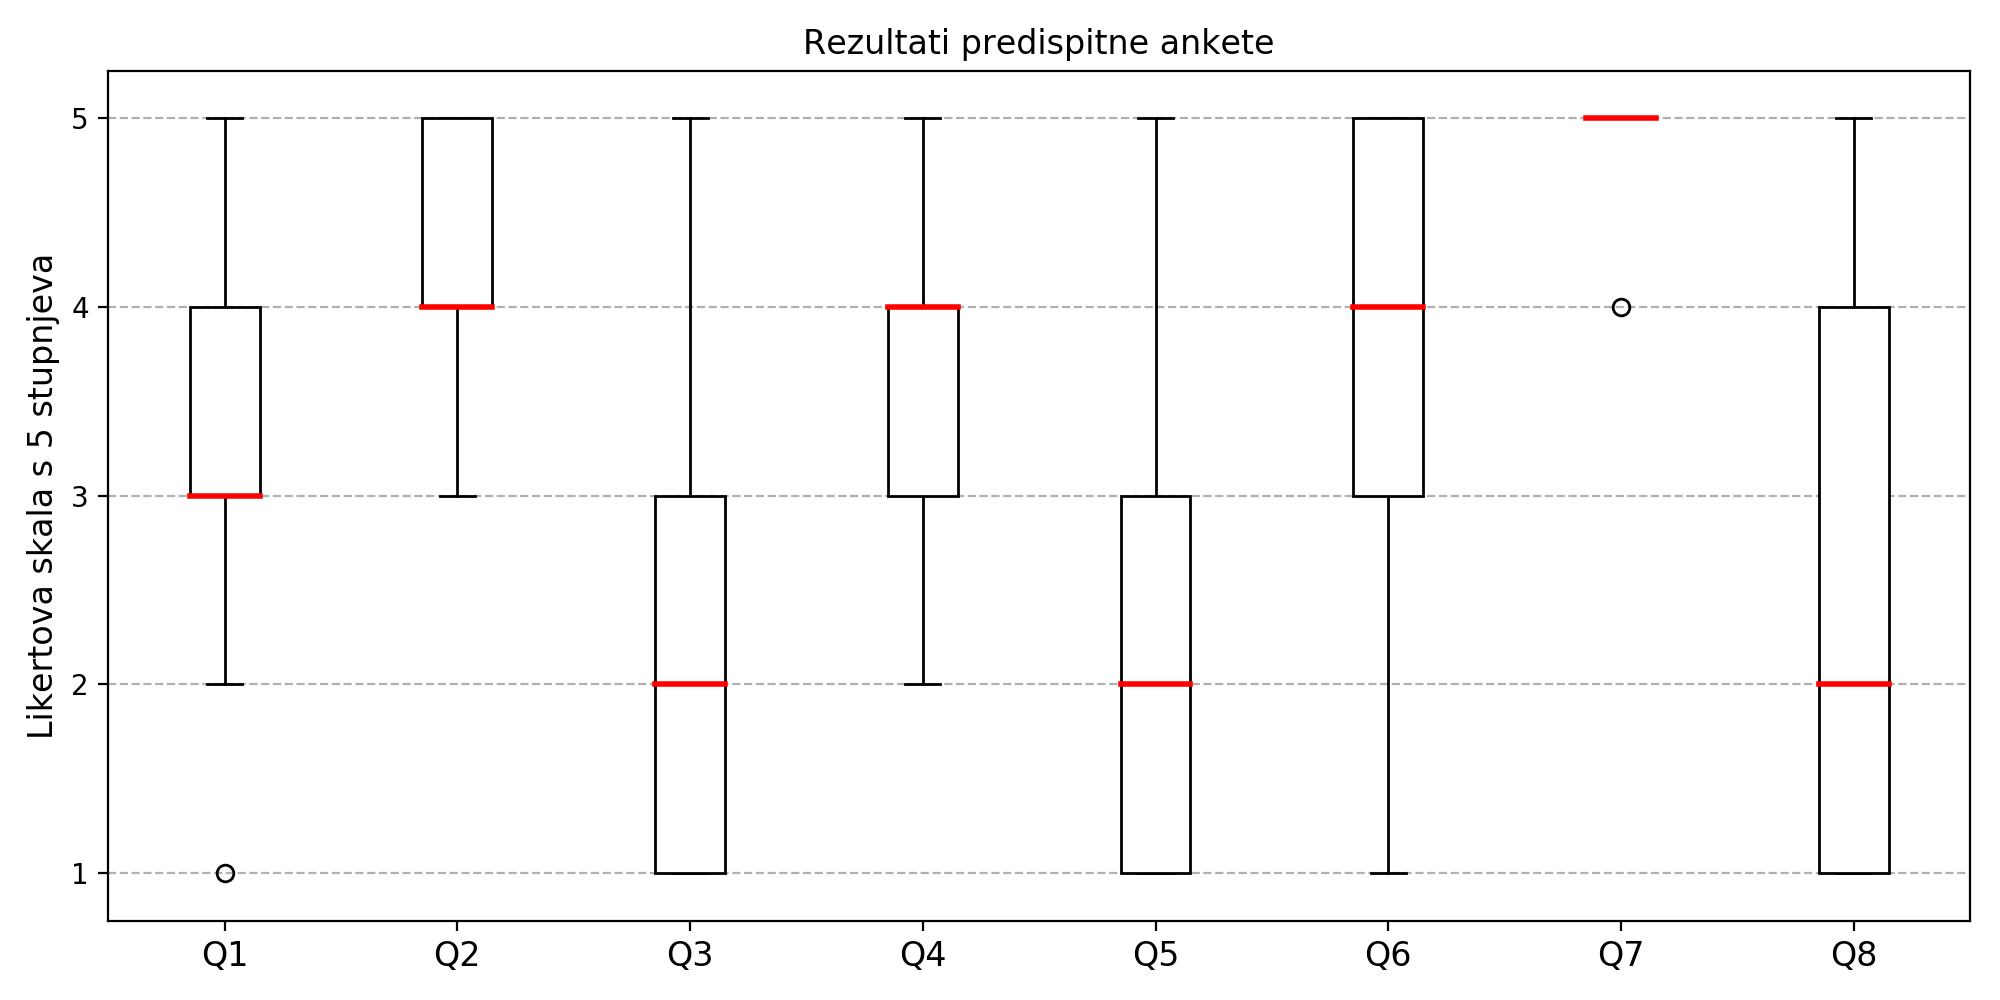
\includegraphics[scale=0.60]{predispitna_anketa_box_whiskers}
		\caption{Box-Whiskers graf s prikazom rezultata predispitne ankete}
		\label{fig:preex_poll}
	\end{center}
\end{figure}

Na slici \ref{fig:preex_poll} mo�emo vidjeti rezultate predispitne ankete u \textit{Box-Whiskers} obliku. Pitanja su ozna�ena s \textbf{Q1} do \textbf{Q8} zbog preglednosti grafa. Odgovori na pitanja su ponu�eni u obliku Likertove skale s 5 stupnjeva. Pitanja glase:

\begin{itemize}
\item \textbf{Q1} - U programima koje �esto koristim, tipkovni�ke kratice u�im: rijetko - �esto
\item \textbf{Q2} - U svakodnevnom radu - Tipkovni�ke pre�ace: uop�e ne koristim - u�estalo koristim
\item \textbf{Q3} - U svakodnevnom radu - Paletu komandi ili ostale alternativne unose pre�aca: uop�e ne koristim - u�estalo koristim
\item \textbf{Q4} - Moje iskustvo u kori�tenju - Tipkovni�kih pre�aca je: malo - veliko
\item \textbf{Q5} - Moje iskustvo u kori�tenju - Palete komandi ili ostalih alternativnih unosa pre�aca je: malo - veliko
\item \textbf{Q6} - Kori�tenje aplikacija - Ure�iva� teksta (Microsoft Word, LibreOffice Writer, . . . ) u radu koristim: rijetko - �esto
\item \textbf{Q7} - Kori�tenje aplikacija - Web preglednik (Google Chrome, Mozilla Firefox, . . . ) u radu koristim: rijetko - �esto
\item \textbf{Q8} - Ure�iva� slika (GIMP, Photoshop, . . . ) u radu koristim: rijetko - �esto
\end{itemize}

Iz dobivenih rezultata mo�e se zaklju�iti kako ispitanici �esto koriste tipkovni�ke pre�ace jer su prepoznali njihovu vrijednost pri olak�avanju rada s ra�unalom. Me�utim, pokazuje se osrednji interes za svjesnim u�enjem pre�aca te mali interes za uporabom raznih pomo�nih alata kao �to je paleta komandi.

Iskustvo u kori�tenju tipkovni�kih pre�aca je veliko, no znanje o raznim alternativnim alatima koji slu�e ubrzavanju rada za ra�unalom je malo. Primjerice, tek je dvoje ispitanika u neformalnom razgovoru priznalo kako ima iskustva u radu s Unity HUD-om a ukupno je �etiri ispitanika odgovorilo s �etvrtim ili ve�im stupnjem na pitanje \textbf{Q5}.

Zadnja tri pitanja odnose se na iskustvo u uporabi programa koji se koriste unutar samog ispitivanja. O�ekivano, uporaba internetskog preglednika je na uvjerljivoj razini, dok je uporaba ure�iva�a teksta na solidnoj razini. Budu�i da se ciljana skupina ispitanika ne bavi u velikoj mjeri obradom slika, razina iskustva kod ure�iva�a slika je niska.

\section{Rezultati zadatka eksperimenta}

\subsection{Vrijeme izvr�avanja zadatka}

\begin{figure}[!htbp]
	\begin{center}
		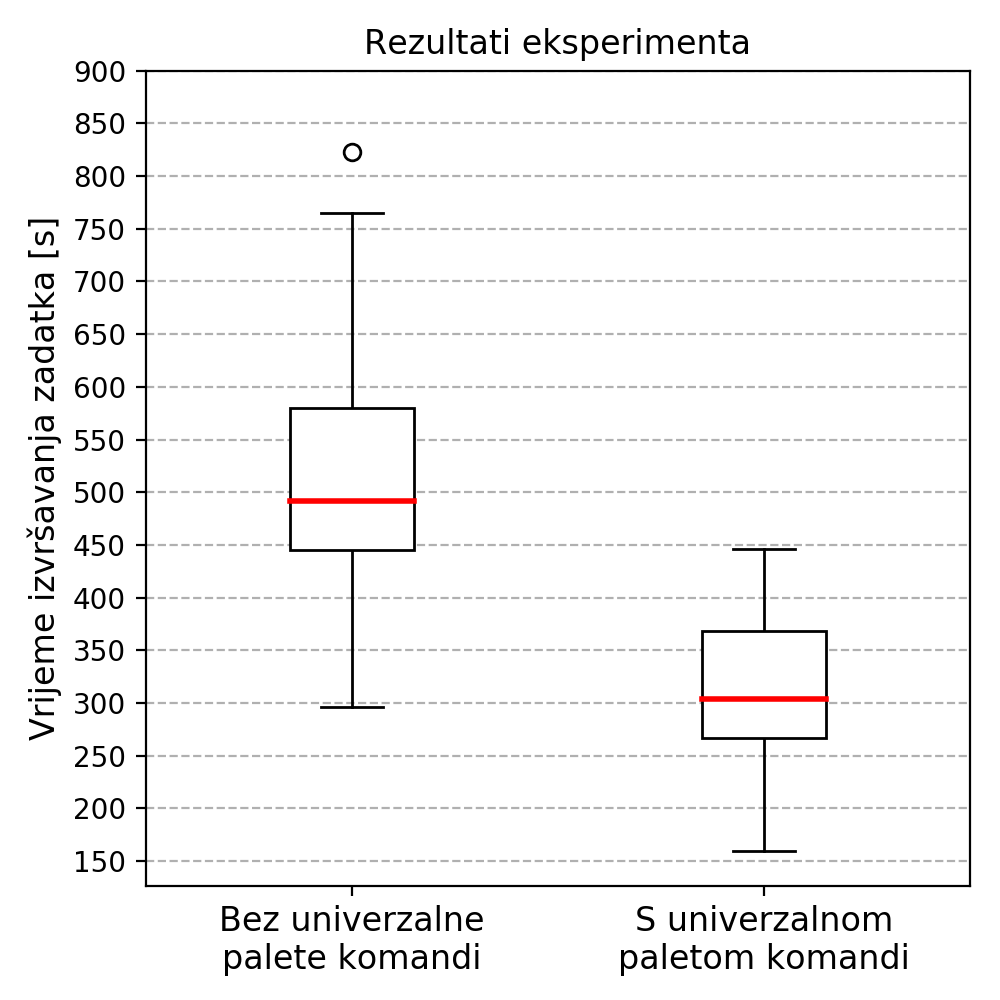
\includegraphics[scale=0.60]{eksperiment_vremena_box_whiskers}
		\caption{Box-Whiskers graf s prikazom vremena izvr�avanja eksperimenta}
		\label{fig:aacp_times}
	\end{center}
\end{figure}

Na slici \ref{fig:aacp_times} vidljiv je \textit{Box-Whiskers} graf koji prikazuje vremena izvr�avanja eksperimentalnog zadatka za prvi i drugi modalitet rada. Konkretno, prosje�na vremena i standardne devijacije iznose:

\begin{itemize}
\item prvi modalitet - bez palete komandi - $ 515,038 \pm 127,743 $ s
\item drugi modalitet - s paletom komandi - $ 310,499 \pm 69,239 $ s
\end{itemize}

Uzimaju�i u obzir prosjek, ispitanicima je s paletom komandi na raspolaganju bilo potrebno �ak pribli�no $ 50\% $ manje vremena za rje�avanje eksperimentalnog zadatka. Tako�er, prona�ena je statisti�ki signifikantna razlika (t-test: t(30)=9,089, df=29, p=$5,5*10^{-10}$ (p $<$ 0,05)), \textit{two-tailed}) izme�u dva modaliteta rada. Potrebno je tako�er napomenuti kako se dio vremena koristi za �itanje samog ispitnog zadatka. Mo�e se zaklju�iti kako dostupnost palete komandi zaista ubrzava rad na ra�unalu.

\subsection{U�estalost uporabe univerzalne palete komandi}

\begin{figure}[!htbp]
	\begin{center}
		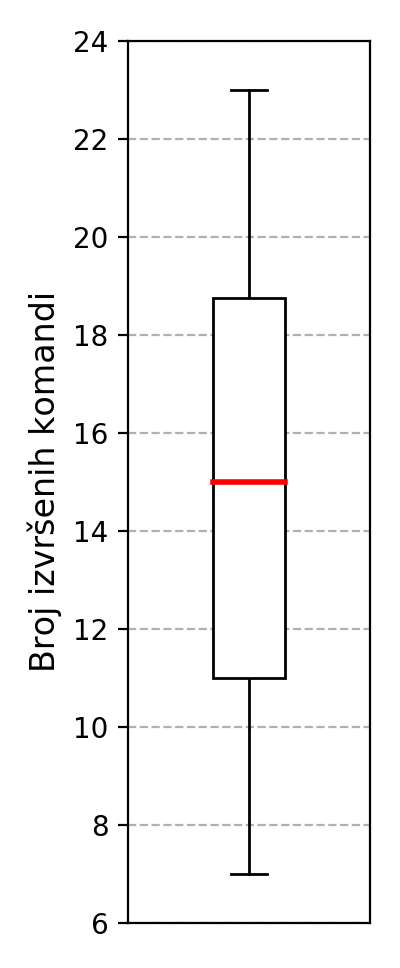
\includegraphics[scale=0.3]{eksperiment_zadaci_box_whiskers}
		\caption{Box-Whiskers graf s prikazom broja iskori�tenih komandi}
		\label{fig:aacp_commands}
	\end{center}
\end{figure}

Za vrijeme eksperimenta se u pozadini vr�ilo bilje�enje komandi koje je ispitanik koristio. Ti su podaci zatim obra�eni tako da su uklonjeni svi duplikati i nepotrebne komande. Eksperiment je bio takav da se niti jedna komanda nije trebala koristiti vi�e puta.

\textit{Box-Whiskers} graf sa slike \ref{fig:aacp_commands} pokazuje kako je svaki ispitanik, za vrijeme drugog modaliteta rada, upotrijebio minimalno 7 komandi. Prosje�ni broj, kao i standarda devijacija je $ 14,77 \pm 4,64 $ distinktnih komandi. Ukupni broj aktivnosti za koje se mogla iskoristiti paleta u sklopu eksperimentalnog zadatka je 24. Mo�e se zaklju�iti kako su ispitanici u pribli�no $ 62\% $ prilika upotrebljavali univerzalnu paletu komandi.

\chapter{Budu�i rad na univerzalnoj paleti komandi}

Mnogi ispitanici su izrazili �elju za kori�tenjem univerzalne palete komandi u svom svakodnevnom radu. Prototip koji je kori�ten u ispitivanju ne sadr�ava mnoge funkcionalnosti koje su nu�ne kako bi se paleta mogla �iroko distribuirati kao aplikacija oko koje bi se stvorila zajednica korisnika. Neke od ideja za budu�nost ovog softvera su:

\begin{itemize}
\item Uporaba razvojnog okvira za \textit{desktop} aplikacije koji ima ve�u zajednicu i podr�ku (primjerice, \textbf{Qt} \cite{17_2019} ili \textbf{Electron} \cite{18_2019}) te mogu�nost razvoja za vi�e \textit{desktop} platformi (Windows, MacOS, Linux).
\item Razvoj ure�iva�a JSON datoteka koje definiraju komande za svaki program.
\item Razvoj centralnog \textit{web} repozitorija za JSON datoteke komandi.
\item Rje�avanje izazova i uvo�enje pobolj�anja navedenih u poglavlju \ref{sec:challenges}:
	\begin{itemize}
	\item Podr�ka funkcionalnostima koje nisu pokrivene standardnim tipkovni�kim pre�acima
	\item Ispravna detekcija bilo kojeg programa
	\end{itemize}
\item Podr�ka za automatsko pokretanje na po�etku rada sustava.
\item Podr�ka za sakrivanje aplikacije unutar \textit{system tray} dijela radne povr�ine na Windows operacijskim sustavima te na ekvivalentima u Linux i MacOS sustavima.
\item Podr�ka za nadogradnjom aplikacije.
\item Implementacija raznih postavki poput:
	\begin{itemize}
	\item Podr�ke za razli�ite jezike
	\item Veli�ine i vrste fonta u aplikaciji
	\item Maksimalnog broja komandi vidljivih u bilo kojem trenutku
	\item Pre�aca za poziv palete komandi
	\end{itemize}
\item Promid�ba aplikacije na Internetu i stvaranje zajednice koja bi pru�ila pomo� pri izradi JSON datoteka komandi i razvoju same aplikacije. U tom slu�aju, univerzalna paleta komandi bi mogla biti aplikacija otvorenog koda.
\end{itemize}
\chapter{Zaklju�ak}

Osnovni cilj zadatka ovog diplomskog rada, koji podrazumijeva implementaciju univerzalne, pro�irive palete komandi i njenu evaluaciju u sklopu eksperimentalnog istra�ivanja je uspje�no postignut. Prototip palete koji je nastao u sklopu ovog rada tako�er ima i svoju ina�icu za Windows operacijske sustave �to predstavlja veliku prednost u odnosu na ista ili sli�na rje�enja navedenima na po�etku ovog rada. 

Jednostavan koncept na kojem po�iva ova paleta pokazao se vrlo uspje�nim, �emu svjedo�e i izvrsni rezultati istra�ivanja. Ispitanici su iskazali zadovoljstvo upotrebljivo��u ove aplikacije te �elju za njenom uporabom u svom svakodnevnom radu. Potvr�ena je signifikantna razlika i osjetno br�i rad za ra�unalom kada je paleta na raspolaganju. Osim svoje osnovne funkcionalnosti, paleta tako�er poma�e korisnicima da nau�e tipkovni�ke pre�ace koje prethodno nisu znali napamet. Na taj na�in, rad za ra�unalom postaje jo� u�inkovitiji jer su pre�aci br�i od pozivanja palete i tra�enja odgovaraju�e komande.

Zaklju�no, jednostavnost i u�inkovitost upotrebe te iznimno pozitivni dojmovi ispitanika optimisti�an su pokazatelj da bi cjelovita, produkcijska i odr�avana verzija palete komandi mogla nai�i na �iroku primjenu i popularnost kod korisnika stolnih ra�unala.

%I) rucno upisati svaku referencu redoslijedom kojim se prvi puta pozivaju u tekstu
%\begin{thebibliography}{99}
%
%\bibitem{html} .....opis reference .........
%
%\bibitem{php} .......opis reference ........
%
%\bibitem{ajax}  .........opis reference..........
%
%\end{thebibliography}


%II) bolji nacin: pomocu programa JabRef opisati svoje reference i pohraniti u datoteku ``Literatura.bib''. U tekstu samo pozivati zeljene reference, a lista se sama formira.

\bibliographystyle{tex_aux/IEEEtranHR}  % ``unsrt'', ``IEEEtran'', ``ieeetr''
% argument is your BibTeX string definitions and bibliography database(s)

\bibliography{Literatura}
  % ovo je ime Bibtex datoteke koju korisnik kreira

%:::::::::: ukljucenje popisa kratica u tekst ::::::::
% Blok linija koda ispod ovoga generira ukljucenje popisa kratica u tekstu. Za uporabu, vidjeti Upute.
% Nije obavezno. Ako se ne zeli koristiti, onda ovaj blok staviti u komentar pomocu znaka %
%\printglossary[type=\acronymtype]
%\pagestyle{plain}
%\begin{glossary}{Longest string}
%	%%%%%%%%%%%%%%%%%%%%%%%%%%%%%%%%%%%%%%%%%%%%%%%%%%%%%%%%%%%%%%%%%%%%%%%%%%%%%%%%%%%%%%%%%%%%%%%%%
%% ovo je jednostavniji (ali neautomatski) primjer definiranja liste akronima, a student neka to zamijeni svojim kraticama i doda sve koje zeli
%% ako se ne zeli deklarirati popis kratica, onda ga staviti pod komentar u glavnoj datoteci
%
%   \item[{\bf HTML}]	Hypertext Markup Language
%   \item[{\bf AJAX}]	Asynchronous JavaScript and XML

%%%%%%%%%%%%%%%%%%%%%%%%%%%%%%%%%%%%%%%%%%%%%%%%%%%%%%%%%%%%%%%%%%%%%%%%%%%%%%%%%%%%%%%%%%

%%%%%%%%%%%%%%%%%%%%%%%%%%%%%%%%%%%%%%%%%%%%%%%%%%%%%%%%%%%%%%%%%%%%%%%%%%%%%%%%%%%%%%%%%%
% Sofisticiraniji nacin definiranja i uporabe kratica je preko sljede?e sintakse

\addcontentsline{toc}{chapter}{Pojmovnik}
% primjeri definicije kratica
% ove pojmove zamijenite nekim svojima i po tom predlosku nadogradite listu po potrebi
%\newacronym{nfc}{NFC}{Near Field Communication}
%\newacronym{wlan}{WLAN}{Wireless Local Area Network} 
%\newacronym{gsm}{GSM}{Global System for Mobile (Communications)}

\newacronym{aacp}{AACP}{Application-Aware Command Palette}

%::::::::: UPORABA KRATICA U TEKSTU :::::::::::::::::
% u tekstu jednostavno na mjestu gdje ?elite koristiti odre?enu kraticu, upotrijebite naredbu 
%  \gls{id_kratice}, kao npr. \gls{nfc}
% i u tekstu ?e vam automatski biti uba?ena kratica kako je definirana u drugoj zagradi u gornjim definicijama, a ako je u uporabi prvi puta, tada ?e prvo biti naveden puni naziv, kako je definiran u tre?oj zagradi, a potom kratica. Za sve ostale slu?ajeve uporabe, bit ?e navedena samo kratica.

%:::::::::::::::::::::::::::::::::::::::::::::::::::::
%  podsjetnik nekoliko mogu?ih oblika sintakse
% op?a uporaba: \gls{nfc} % mo?e i za rje?nik i za kratice. Prvi poziv daje dugi i kratki naziv (redoslijedom koji je specificiran u preambuli pomocu \setacronymstyle, a od drugi puta nadalje samo kraticu.
% ako ?elite nametnuti ba? neki oblik kori?tenja kratice, imate sljede?e naredbe
%\acrshort{nfc} \\  % samo akronim
%\acrfull{nfc} \\   % akronim i puni naziv
%\acrlong{nfc} \\   % samo puni naziv

%::::::::::::::::::::::::::::::::::::::::::::::::::::
% Kako se generira Pojmovnik u tekstu:
%1. pokrenite LaTeX kompilaciju 1x
%2. u Command Promptu odite radnu mapu gdje su vam datoteke diplomskog rada i utipkajte
%	makeindex -s myDoc.ist -o myDoc.gls   myDoc.glo
%	
%	gdje myDoc zamijenite imenom svoje glavne .tex datoteke (JMBAG_Ime_Prezime.tex)
%3. pokrenite LaTeX kompilaciju jos jednom

%::::::::::::::::::::::::::::::::::::::::::::::::::::
%\end{glossary}

%:::::::::::: blok za definiranje Sazetka/Abstracta rada 
\begin{abstract}
	\vspace{5pt}

%:::::::::::::::::::::::::::::::::::::::::::::::::::::
%:::::::::::: HRVATSKI :::::::::::::::::::::::::::::::
U sklopu ovog rada implementirana je univerzalna i pro�iriva paleta komandi. Paleta mo�e raditi s bilo kojim programom koji podr�ava tipkovni�ke pre�ace. Poziva se na prethodno pode�eni tipkovni�ki pre�ac, prepoznaje program koji se treutno upotrebljava te nudi pretra�ivi popis komandi koje se mogu izvr�iti unutar tog programa. Svaka komanda se izvr�ava njenim odabirom i pritiskom na tipku Enter, �ime paleta emulira odgovaraju�i tipkovni�ki pre�ac �to rezultira izvr�avanjem odre�ene radnje. Mogu�e je napisati nove popise komandi za bilo koji drugi program. Tako�er, provedeno je istra�ivanje upotrebljivosti univerzalne palete komandi u kojem je sudjelovalo trideset ispitanika. Rezultati sugeriraju osjetno pove�anje u�inkovitosti svakodnevnog rada za ra�unalom. U sklopu istra�ivanja ispitanici su radili s internetskim preglednikom \textit{Chrome}, ure�iva�em teksta \textit{LibreOffice Writer} i ure�iva�em slika \textit{GIMP}. Dojmovi ispitanika o upotrebljivosti, prema standardiziranom upitniku SUS, su tako�er vrlo pozitivni.
%:::::::::::::::::::::::::::::::::::::::::::::::::::::

\vspace{5pt}
%
\noindent \textbf{\textit{Klju�ne rije�i} --- interakcija �ovjeka i ra�unala, paleta komandi, tipkovni�ki pre�aci, produktivnost, univerzalnost, pro�irivost, platformska nezavisnost} 

%:::::::::::: KRAJ HRVATSKOG DIJELA :::::::::::::::::::


%::::::::::::::::::::::::::::::::::::::::::::::::::::::
%:::::::::::: ENGLESKI ::::::::::::::::::::::::::::::::

%\vspace{-10pt}
\section*{Abstract}
\vspace{-10pt}
Within this master's thesis, a universal and extendable command palette was implemented. The palette can be used with any software which supports keyboard shortcuts. It can be invoked with a previously configured keyboard shortcut, it recognizes the program which is currently being used and it offers a searchable list of commands which can be executed inside that program. Each command is executed by selecting it and pressing Enter, after which the palette emulates corresponding keyboard shortcut which results in the execution of a certain task. It is possible to write new command lists for any other application. Also, experimental research on usability of the universal command palette in which thirty participants were involved was conducted. Results suggest a significant increase in everyday computer work efficiency. Within the research, participants worked with web browser \textit{Chrome}, text editor \textit{LibreOffice Writer} and image editor \textit{GIMP}. Impressions from participants regarding usability, from the standardized SUS measure, are also very positive.
%:::::::::::::::::::::::::::::::::::::::::::::::::::::::

\vspace{5pt}
%
\noindent \textbf{\textit{Keywords} --- human-computer interaction, command palette, keyboard shortcuts, productivity, universality, extendability, platform independence}

%::::::::::::::::::::::::::::::::::::::::::::::::::::::
%:::::::::::: KRAJ ENGLESKOG DIJELA :::::::::::::::::::

	  % sazetak rada i kljucne rijeci na HR i EN
\end{abstract}

%:::::::::::: PRILOZI (neobavezno) ::::::::::::::::::::
% ispod \appendix zaglavlja pomocu \include dodati poglavlja s prilozima
% ukoliko nemate priloga, ovaj blok linija staviti u komentar
\appendix
\chapter{Ispitni materijali}

Ispitni materijali se nalaze na sljede�im stranicama. Imaju ukupno devet stranica, od kojih one s tekstom zadatka nisu bile dostupne ispitanicima ali su svejedno slu�ile za povremenu ispomo�. Materijali su prikazani u originalnom obliku, zajedno s numeriranim stranicama.
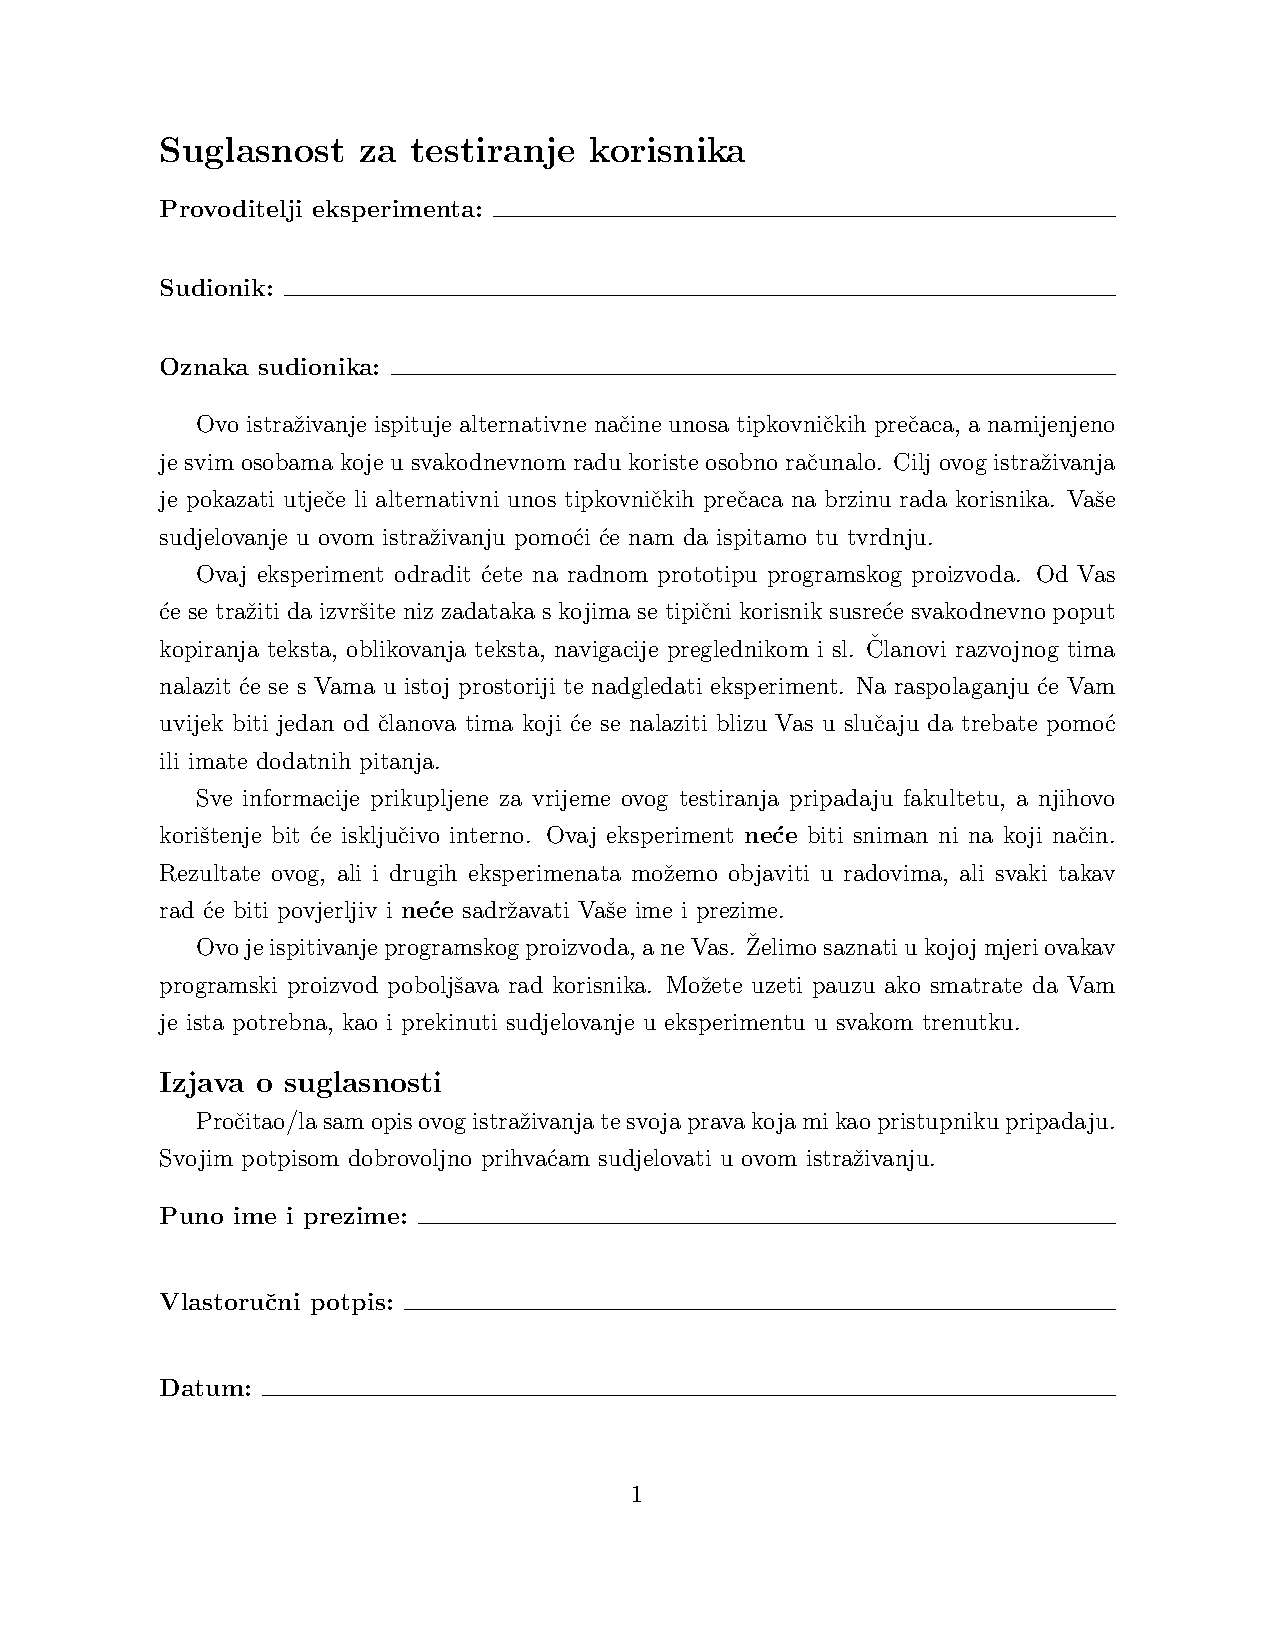
\includepdf[pages=-]{expdocs.pdf}  % dati neko suvislo ime umjesto ovoga
%\include{Prilog_2}  % itd.

\end{document}
